\documentclass[a4paper,12pt,oneside,fleqn]{book}


\usepackage[T1]{fontenc}
\usepackage[utf8]{inputenc}
\usepackage{graphicx}
\usepackage{xcolor}
\usepackage{mathptmx}
\usepackage[colorlinks = true, linkcolor = blue]{hyperref}

%algorithm
\usepackage{algpseudocode}

\usepackage{amsmath,amssymb,amsthm,textcomp}
\usepackage{multicol}
\usepackage{tikz}
\usepackage[normalem]{ulem}
\usepackage{bbm} % using for the characteristic function
\usepackage{ulem}
\usepackage{cancel}
\usepackage{esint} %integral mean

\usepackage{geometry}
\geometry{left=10mm,right=10mm,%
bindingoffset=0mm, top=10mm,bottom=15mm}



\renewcommand{\thechapter}{\Roman{chapter}}
\renewcommand*\thesection{\arabic{section}}


%\newtheorem{theorem}{Theorem}
\newtheorem{theorem}{Theorem}[section]
\newtheorem{algorithm}{Algorithm}[section]
\renewcommand{\thetheorem}{\arabic{section}.\arabic{theorem}}
\newtheorem{corollary}{Corollary}[theorem]
\newtheorem{lemma}[theorem]{Lemma}
\newtheorem{proposition}[theorem]{Proposition}
\newtheorem{method}[theorem]{method}

\theoremstyle{definition}
\newtheorem{definition}{Definition}[section]
\renewcommand{\thedefinition}{\arabic{section}.\arabic{definition}}

\newtheorem*{example}{Example}
\newtheorem{assumption}{Assumption}[section]
\newtheorem{exercise}{Exercise}[chapter]
\theoremstyle{remark}
\newtheorem*{remark}{Remark}
\newtheorem{review}{Review}

%contradiction
\usepackage{marvosym}

\linespread{1.3}
\newcommand{\linia}{\rule{\linewidth}{0.5pt}}


% my own titles
\makeatletter
\renewcommand{\maketitle}{
\begin{center}
\vspace{2ex}
{\huge \textsc{\@title}}
\vspace{1ex}
\\
\linia\\
\@author \hfill \@date
\vspace{4ex}
\end{center}
}
\makeatother
%%%

% custom footers and headers
\usepackage{fancyhdr}
\pagestyle{fancy}
\lhead{}
\chead{}
\rhead{}
\lfoot{}
\cfoot{}
\rfoot{\thepage}
\renewcommand{\headrulewidth}{0pt}
\renewcommand{\footrulewidth}{0pt}
%

% code listing settings
\usepackage{listings}
\lstset{
    language=Python,
    basicstyle=\ttfamily\small,
    aboveskip={1.0\baselineskip},
    belowskip={1.0\baselineskip},
    columns=fixed,
    extendedchars=true,
    breaklines=true,
    tabsize=4,
    prebreak=\raisebox{0ex}[0ex][0ex]{\ensuremath{\hookleftarrow}},
    frame=lines,
    showtabs=false,
    showspaces=false,
    showstringspaces=false,
    keywordstyle=\color[rgb]{0.627,0.126,0.941},
    commentstyle=\color[rgb]{0.133,0.545,0.133},
    stringstyle=\color[rgb]{01,0,0},
    numbers=left,
    numberstyle=\small,
    stepnumber=1,
    numbersep=10pt,
    captionpos=t,
    escapeinside={\%*}{*)}
}
\DeclareMathAlphabet{\mathcal}{OMS}{cmsy}{m}{n}

%symbol
\AtBeginDocument{
  \let\ran\relax
  \DeclareMathOperator{\dom}{dom}
}\AtBeginDocument{
  \let\ran\relax
  \DeclareMathOperator{\ran}{ran}
}
\DeclareMathOperator{\var}{Var}


\AtBeginDocument{
  \let\div\relax
  \DeclareMathOperator{\div}{div}
}



\DeclareMathOperator*{\esssup}{ess\, sup}
\DeclareMathOperator*{\spa}{span}
\DeclareMathOperator*{\dist}{dist}
\DeclareMathOperator*{\diam}{diam}
\DeclareMathOperator*{\interior}{int}
\DeclareMathOperator*{\conv}{conv}
\DeclareMathOperator*{\refine}{Ref}

%%%----------%%%----------%%%----------%%%----------%%%

\begin{document}
\title{Numerica}
\author{Ruizhe Chao}
\date{\today}
\maketitle
\tableofcontents



\chapter{Numerical Linear Algebra}
Given the increment method $ z_N(t_{i + 1}) = \Phi(t_i, z_i, h_i)$  for the lattice function $z_N$, we decompose the error as:
\begin{align*}
	\|z_N(t_{i + 1}) - z(t_{i + 1})\| &= \|\Phi(t_i, z_N(t_i), h_i) - z(t_{i + 1})\|\\
	&\le \| \Phi(t_i, z_N(t_i), h_i) - \Phi(t_i, z(t_i), h_i)\|
	 + \|\Phi(t_i, z_N(t_i), h_i)  - z(t_{i + 1})\|
\end{align*}


\section{Power of linear endomorphism}


\section{Numerical precision}
\begin{definition}[condition number]
Given a problem $f$ and $\delta f:= f(x) - f(\tilde{x})$ the relative error. the condition number is defined as 
\begin{equation}
	\lim_{\epsilon \rightarrow 0} \sup_{\|\delta x\|< \epsilon} \frac{\delta\|f(x)\|}{\|\delta x\|},
\end{equation}
in particular, the condition number of a matrix $A$ is defined as
\begin{equation}
	\kappa(A) = \frac{\lambda_{max}}{\lambda_{min}}
\end{equation}
\end{definition}

\begin{definition}[Stability]
	A one-step method $\Phi$ is called stable if it is insensitive w.r.t. small perturbation of the state, i.e.,  
	\begin{align*}
		\| \Phi(t_i, z_1, h_i) - \Phi(t_i, z_2, h_i)\| \le C \|z_1 - z_2\|
	\end{align*}
	for some constant $C$. 
\end{definition}

\begin{definition}[Consistency]
	A numerical method is consistent if it converges as the stepsize tends to 0, i.e., 
	\begin{align*}
		\|\Phi(t_i, z_N(t_i), h_i)  - z(t_{i + 1})\|\le  \epsilon(h) h
	\end{align*}
	The algorithm admits the consistent order $p$, if 
	\begin{align*}
		\epsilon(h) = C\epsilon^p
	\end{align*}
\end{definition}




\section{The Nonlinear System of Equations}
\begin{lemma}[Neumann's lemma]
	Given $B \in \mathbb{R}^{n \times n}$ with $\|B\| \le q < 1$. Then $(I - B)$ is invertible and 
	\begin{equation}
		\|(I - B)^{-1}\| \le \frac{1}{1 - q}
	\end{equation}
\end{lemma}

\begin{algorithm}[The Newton method]
Given $f: \mathcal{D} \rightarrow \mathbb{R}^d$ continuously differentiable. 
\begin{algorithmic}
\State $x_0 \in \mathcal{D}$
\While{$\|\nabla f(x)\| \ge \epsilon$}
\State $x_{k + 1} = x_k - \frac{f(x_k)}{\nabla f(x_k)}$. 
\EndWhile
\end{algorithmic}
\end{algorithm}

\begin{theorem}[Local convergence of the Newton method]
	Given $f \in C^1(\mathcal{D}, \mathbb{R}^m)$, the Newton method converges linearly. 
	If $\nabla f \in Lip(\mathcal{D}, \mathbb{R}^m)$, the method converges quadratically. 	
\end{theorem}

\section{Interpolation}
\subsection{Polynomial Interpolation}
Observe the \textbf{Lagrange Polynomial}:
\begin{equation}
	L_j(x_i) = 
	\left\{
	\begin{aligned}
		1 \qquad i = j\\
		0 \qquad i \neq j
	\end{aligned}
	\right.
\end{equation}
given by
\begin{align*}
	L_j(x) = \prod_{i \neq j} \frac{x - x_i}{x_j - x_i}
\end{align*}
\begin{definition}[Interpolation polynom]
	We define the Lagrange-interpolation polynomial:
\begin{align*}
	p_n(x) &= \sum_{i = 0}^n y_i L_i(x) \quad \textbf{(1)}\\
	&= \sum_{k = 0}^n y[x_0, \dots, x_k] \prod_{j = 0}^{k - 1} (x - x_j) \quad \textbf{(2)}
\end{align*}
where we call \textbf{(1)} the Lagrangian and \textbf{(2)} the Newton Interpolation polynom.
\end{definition}

\begin{algorithm}[Lagrange interpolation]
Given $n$ pair of points $(x_i, y_i)$, $i = 1, \dots, n$. 
\begin{algorithmic}
\For{i = 1, \dots, n}
\State $L_j(x) = L_j[x_1, \dots, x_n](x)$, \text{ as in the definition}
\State $p(x) = \sum_{i = 1}^n y_i L_i(x).  $
\EndFor
\end{algorithmic}
\end{algorithm}


\begin{theorem}[The interpolation error]
Given $f \in C^{n + 1}(D)$ and $I = [x_0, \dots x_n]$ a partition of $D$, we have
\begin{align*}
	f(x) - p_n(x) \le \frac{\partial^{n + 1}_t f(\theta_t)}{(n+1)!} \prod_{i = 0}^n (x - x_i) = \mathcal{O}(h^{n + 1}) \text{ with } \theta_t \in [x_0, x_n].
\end{align*}
\end{theorem}

\subsection{Splines}


\chapter{Numerical ODE}

\section{Exam Questions}
\begin{enumerate}
	\item Under what conditions do the explicit RK-methods admit the consistence order of 1 and prove the statement.\\
	If $ \sum b_1 = 1$. Included in the usual compatibility condition.
	\item Under what conditions do RK-methods admit consistence order of $p$?
	\item Under what conditions do RK-methods converges?
\end{enumerate}

\section{Numerical Integration}
Consider 
\begin{align*}
	x(t) = x(0) + \int_0^t f(s) ds
\end{align*}
want to calculate $x(t)$.

\begin{definition}[The Quadrature formula]
Given the notes over the interval $[0, T]$: $0 = t_0 < t_1 \dots < t_n = T$, we define the \textbf{quadrature formula} of integration as 
 we use the \textbf{quadrature formula}:
\begin{align*}
	Q(f) = \sum_{ i = 0}^n w_i f(t_i).
\end{align*}
it holds
\begin{align*}
	Q(f) \approx I(f) = \int_0^t f ds + f(0)
\end{align*}
\end{definition}
Choosing the equidistant nodes, the quadrature formula for n nodes a corresponds to certain naming formula
\begin{enumerate}
	\item $n = 0$: $Q(f) =  (\beta - \alpha) ds$. 
	\item $n = 1$ (\textbf{Traproid rule)}:  $Q(f) = \frac{h}{2}f(\alpha) + \frac{h}{2} f(\beta)$.  
	\item $n = 2$ (\textbf{Simpson rule}): $Q(f) = \frac{h}{6}\bigg( f(a) + 4 f(\frac{a + b}{2}) + f(b) \bigg).$
\end{enumerate}
\begin{remark}
\qquad\\
\textbf{1.} Simpson rule is the Lagrange formula with 3 equidistant knots. 
\end{remark}



\subsection{Quadrature Error of Lagrange formula}
\begin{theorem}[quadrature error with $n + 1$ nodes]
	Given $f \in C^{n + 1}(a, b)$, the quadrature formula admits the   error:
	\begin{equation}
		|R(f)| \le \max_{\theta \in [a, b]} \frac{\partial^{n + 1}_t f(\theta)}{(n + 1)!} (b - a)^{n + 2}. 
	\end{equation}
\end{theorem}
\begin{proof}
Recall the interpolation error of the Lagrange interpolation. For $f \in C^{n + 1}(a, b)$ and the interpolation $p \in P_n$ with $n + 1$ nodes, we have  $\forall t \in [a, b] \exists \theta_t$: 
\begin{equation}
	f(t) - p_n(t) = \frac{\partial^{n + 1}_t f(\theta_t)}{(n+1)!}(t - t_0) \dots (t - t_n). 
\end{equation}
Taking integration over $[a, b]$ we have
\begin{equation}
	R(f)  \le \max_{ \theta \in [a, b]} \frac{\partial_t^{n + 1} f(\theta)}{(n + 1)!}  \underbrace{\int_a^b (b - a)^{n + 1} dt}_{ = (b - a)^{n + 2}}.  
\end{equation}
\end{proof}

\begin{corollary}
	The Lagrange formula with $n + 1$ knots admits at least the algebraic precision level of $n$ 
\end{corollary}

\begin{corollary}
	The righthand rule admits the algebraic precision level of 0. 
\end{corollary}

Notice that the error doesn't go to 0 as we decrease the mesh size, hence we introduce the \textbf{composite integration formula}, where we estimate $(\beta - \alpha)$ by $h$ and the error converges to 0 as $h$ tends to 0. 






\subsection{Algebraic Precision Level}
\begin{definition}[exact quadrature formel]
Given a quadrature formula $Q(f)$, we define the \textbf{quadrature error}:
\begin{equation}
	R(f):= |I(f) - Q(f)|. 
\end{equation}
A quadrature formal is \textbf{exact}, if
\begin{align*}
	R(f) = 0.
\end{align*}
\end{definition}
\begin{remark}
In general the quadrature error is not calculable since $I(f)$ is in general not known.
\end{remark}


\begin{definition}[algebraic precision level]
	The quadrature formula admits the \textbf{algebraic precision level} of $\mu$, if it is \textbf{at most} exact for all polynomials of degree of $\mu$, i.e., 
	\begin{align*}
		\forall f \in P_\mu: R(f) = 0, \text{ and }
		\exists g \in P_{\mu + 1}: R(g) \neq 0. 
	\end{align*}
\end{definition}

\begin{lemma}
	The quadrature formula admits the algebraic precision level of $\mu$ if and only if 
	\begin{align*}
		\forall i = 0, \dots, \mu: R(t^i) = 0 
		\text{ and }
		R(t^{\mu + 1}) \neq 0. 
	\end{align*}
\end{lemma}
\begin{proof}
\end{proof}

\begin{remark}
The algebraic precision level depends on the choice of notes. 	
\end{remark}

\begin{lemma}
	A quadrature formula with $n + 1$ nodes admits \textbf{at most} the algebraic precision level of $2n + 1$. 
\end{lemma}
\begin{proof}
	We construct $q(t) \in P_{2n +2}$ such that the quadrature formula cannot be exact, observe
	\begin{align*}
		q(t) = \prod_{j = 0}^n(t - t_j)^2 \ge 0.
	\end{align*}
	It holds
	\begin{align*}
		\int_a^b q	(t)dt \gneqq 0. 
	\end{align*}
	However
	\begin{align*}
		Q(q) = \sum_{i = 0}^n w_j (t_j - t_i)^2 = 0.
	\end{align*}
	Hence
	\begin{align*}
		|R(q)| = |q - Q(q)| > 0. 
	\end{align*}
\end{proof}

\begin{theorem} Given $Q(f)$ the quadrature formula with $n + 1$ knots(which admits the algebraic precision level of at least $n$), $Q(f)$ admits the algebraic precision level of $2n + 1$ if and only if 
\begin{align*}
	\forall q(t) \in P_{n}(a, b): \quad \int_a^b q(t) \prod_{j = 0}^{n + 1} (t - t_j) dt = 0. 
\end{align*}
\end{theorem}
\begin{proof}\quad\\
\textbf{$\Rightarrow$}: $\forall q \in P_n(a, b)$ we have $q(t)\prod_{j = 0}^n (t - t_j) \in P_{2n + 1}(a, b)$, since $Q$ admits the algebraic precision level of $2n + 1$, it holds
\begin{align*}
	\int_a^b q(t)\prod_{j = 0}^{n}(t - t_j)dt - \sum_{j = 0}^n w_j q(t_j)\underbrace{ \prod_{k = 0}^n (t_j - t_k)}_{ = 0} = 0.
\end{align*} 
Therefore 
\begin{align*}
	\int_a^b q(t) \prod_{j = 0}^n (t - t_j) dt = 0. \quad \forall q \in P_n(a, b). 
\end{align*}
$\Leftarrow$: \qquad\\ 
By the polynomial devision we know for $p = \prod_{j = 0}^n(t - t_j)$, 
\begin{align*}
	\forall \bar{p} \in P_{2n + 1}(a, b) \quad \exists q, r \in P_{n}(a, b):\quad \bar{p} = pq + r.
\end{align*}
Hence
\begin{align*}
	I(\bar{p}) &= \underbrace{ \int_a^b pq}_{ = 0}  + \int_a^b r\\
	& = \sum_{j = 0}^n w_j r(t_j)\text{ (since $Q$ exact for $P_n$)}\\
	& = \sum_{j = 0}^n w_j \bigg(\underbrace{ pq(t_j)}_{ = 0} + r(t_j) \bigg). \\
	& = Q(\bar{p}).  
\end{align*}
\end{proof}

\begin{corollary}
	The quadrature formula $Q(f)$ admits the algebraic precision level of $2n + 1$ if and only if 
	\begin{align*}
		\int_a^b \tau^k \prod_{j = 0}^n ( \tau - t_j) d\tau = 0 \quad \forall k = 0, \dots, n. 
	\end{align*}
\end{corollary}



\subsection{Gauss Quadrature Formula}
\subsubsection{Legendre Polynomial}
\begin{definition}[Legendre polynomial]
	For $n \in \mathbb{N}_0$, we define the Legendre polynomial $L_{n + 1} \in P_{n + 1}([-1, 1])$ as  
	\begin{equation}
	\begin{aligned}
		& L_{n + 1}(\tau) = 
	\end{aligned}
	\end{equation}
\end{definition}

\begin{lemma}
	The Legendre polynomial admits the following properties
	\begin{enumerate}
		\item It holds
		\begin{equation}
			\int_{-1}^1 \tau^k L_{n + 1}(\tau) d\tau = 0, \text{ for all } k = 0, \dots, n.  
		\end{equation}
		\item $\{L_1, \dots, L_{n+1}\}$ forms an orthogonal basis of the space $(P_{n + 1}(-1, 1), \langle, \rangle_{L^2(0, 1)})$.  
		\item $L_{n + 1}$ admits $n +1$ \textbf{real} roots over the interval $[-1, 1]$. 
	\end{enumerate}
\end{lemma}
\begin{proof}
\quad\\
\textbf{ad 1.}


\quad\\
\textbf{ad 2.} Argue by contradiction $L_{n + 1}$ admits a complex root $\tau^*$, then $\overline{\tau^*}$ is also a root. Then we have 
\begin{align*}
	L_{n + 1}(\tau) = (\tau - \tau^*)(\tau - \bar{\tau^*})q(\tau), \text{ with } q(t) \in P_{n -1}.
\end{align*}
By the orthogonality of $L_{n + 1}$ we have for $q \in P_{n - 1}$ that
\begin{align*}
	0 = \int_{-1}^1 L_{n+1}(\tau) q(\tau) d\tau = \int_{-1}^1 (\tau - \tau^*)^2 q(\tau)^2 d\tau.
\end{align*}
It follows $q(t) = 0$ and therefore $L_{n + 1} =0$ and we have a contradiction. 
\end{proof}

\begin{definition}[the Gauss quadrature form]
Given $\tau_1, \dots, \tau_{n + 1}$ the roots of the Legrendre polynomial, choose 
\begin{equation}
	t_i = \frac{a - b}{2} \tau_i +  \frac{a + b}{2}. 
\end{equation}	
The quadrature formula 
\begin{align*}
	Q(f) = \sum_{j = 0}^n w_j f(\tau_j), 
	\quad
	w_j = \int_a^b \prod_{i = 0, i \neq j}^n \frac{t - t_i}{t_j - t_i}dt. 
\end{align*}
 is called \textbf{Gaussian quadrature formula}
\end{definition}

\begin{remark}[The knots lie on the interval $\alpha, \beta$]
\begin{proof}
It holds
\begin{align*}
	\alpha \le \frac{\alpha + \beta}{2} + \frac{\beta - \alpha }{2}\tau_j \le \beta. 
\end{align*}
Because $\tau_j \in [0, 1]$. 
\end{proof}
\end{remark}

\begin{theorem}[algebraic precision level of the Gaussian quadrature formula]
	The Gaussian quadrature formula with $n + 1$ knots admit the algebraic precision level of $2n + 1$. 
\end{theorem}
\begin{proof}
	By the theorem above we know 
	\begin{enumerate}
		\item $L_{n + 1} = \prod_{j = 0}^{n + 1} (t - \tau_j)$. 
		\item $\int_a^b \tau^k L_{n + 1} d\tau = 0$ for $k = 1, \dots, n$. 
	\end{enumerate}
\end{proof}

\subsubsection{The composite Gaussian quadrature formula}
\begin{theorem}
	
\end{theorem}





\subsection{The Composite formel}
\subsubsection{The Composite Integration Formula}
The composite integration formula breaks the entire interval into subintervals and then apply the integration over each subinterval. The composite integration formula with $m$ equidistant subinterval and $k+1$ nodes on each subinterval is
\begin{align*}
	\int_a^b f dt = \sum_{i = 1}^m \int_{a_i}^{b_i} f dt
	\approx \sum_{i = 1}^m \int_{a_i}^{b_i} p(t)dt  
	= \sum_{i = 1}^m \sum_{j = 0}^k w_j f(t_j).
\end{align*}

\begin{theorem}
	Given $f \in C^{n + 1}([a, b], \mathbb{R})$, the composite integration formula with $m$ equidistant subinterval and $k + 1$ nodes admits the quadrature error:
	\begin{equation}
		|R(f)| \le \frac{ \max_{x \in [a, b]}| \partial_x^{n + 1} f(x)|}{(n + 1)!} (b - a)h^{n + 1}.
	\end{equation}
\end{theorem}

\section{LMV Of ODEs}
Given a ODE
\begin{equation}
\begin{aligned}
	&x'(t) = f(t, x)\\
	&x(0) = x_0
\end{aligned}
\end{equation}






\subsection{Linear Multistep Method}
The general \textbf{Linear-Multistep-Method(LMM) }with equidistant mesh has the form
\begin{equation}
	 \sum_{i = 1}^k \alpha_{i} x_{n -i} = h \sum_{i = 1}^k \beta_{i} f(t_{n - i}, x_{n -i}).
\end{equation}
\subsubsection{The Adam Method \& BDF Method}
We first introduce the methods with Lagrange methods. 

\subsubsection{Adams-Bashforth}
In general we have
\begin{align*}
	x(t_{n + 1}) - x(t_n) = \int_{t_n}^{t_{n + 1}} f(s, x(s))ds 
\end{align*}
We apply the numerical integration on the RHS with polynomial of \textbf{degree $k - 1$} on the node $t_{n -1}, \dots, t_{n - k}$ , 
\begin{align*}
	x(t_{n + 1}) - x(t_n) = \sum_{j = 1}^{k} \underbrace{\int_{t_n}^{t_{n + 1}} \prod_{i = 1, i \neq j}^k \frac{t - t_{n - i}}{t_{n -j} - t_{n - i}} dt}_{:= \beta_{j}}  f(t_{n - j}, x(t_{n -j})).
\end{align*}
\begin{remark}
In the case of equidistant nodes we have
\begin{align*}
	w_{nj} = h \beta_j.
\end{align*}	
where $\beta_j$ and $h$ are independent. 
\end{remark}


\begin{algorithm}[Adam-Bashforth]
\begin{algorithmic}\quad
\State $x_0 = x(0)$
\For{$j = 1, \dots, N$}
\If{$j \le k$}
\State $x_n = x_{n -1} + h\sum_{j = 1}^{n} \beta_j f(t_{n - j}, x_{n -j})$
\Else
\State $x_n = x_{n -1} + h\sum_{j = 1}^k \beta_j f(t_{n - j}, x_{n - 1})$
\EndIf
\EndFor
\end{algorithmic}	
\end{algorithm}


\subsubsection{Adam-Moulton}
Adam-Moulton is a implicit method, which apply numerical integration of degree $k$ with $k + 1$ nodes on the RHS, i.e., 
\begin{align*}
	x_n = x_{n -1} + \sum_{j = 0}^k \underbrace{\int_{t_{n -1}}^{t_n} \prod_{i = 0, i \neq j}^k \frac{t - t_{n -i}}{t_{n -j} - t_{n - i}} dt}_{:= \beta_{j}} f(t_{n - j}, x(t_{n -j})).
\end{align*}


\begin{algorithm}[Adam-Moulton]
\end{algorithm}


\subsubsection{BDF method}
In a Backward Differential Formulas, instead of interpolating the RHS, we interpolate the LHS with the polynomial of degree $k$ , and take the derivate, i.e., 
\begin{align*}
	\partial_t p_x(t) = \partial_t \bigg( \sum_{j = 0}^k \bigg( \underbrace{ \prod_{i = 0, i \neq j}^k \frac{t - t_{n -i}}{t_{n -j} - t_{n - i}}\bigg)}_{L_{n -j}(t)}x_{n - j} \bigg).  
\end{align*}
We have
\begin{align*}
	\partial_t p_x(t_n) \approx f(t_n, x_n),
\end{align*}
with 
\begin{align*}
	\partial_t p_x(t_n):= \eta_{nj} = \frac{1}{h}\alpha_j,
\end{align*}
for equal-distant knots. 
\begin{align*}
	\sum_{j = 0}^k \frac{1}{h} \alpha_{j} x_{n - j} = f(t_n, x_n). 
\end{align*}
\begin{remark}
In the case of equidistant nodes, we have
\begin{align*}
	\eta_{nj} = \frac{1}{h} \alpha_j, 
\end{align*}	
where $\alpha_j$ and $h$ are independent. 
\end{remark}

\begin{algorithm}[BDF-Method]
\end{algorithm}



\subsection{Consistent Error}
In this subsection we introduce 2 definitions: consistent error and the local error, we see how the consistent error is a gut measure of the local error. 
\begin{definition}[consistency of LMVs]
Given a LMV and a function $x \in C^1 $ the exact solution, we define the consistent error as estimation error at $t_n$:
\begin{equation}
	L_n(x) = \sum_{i = 0}^k \alpha_i x(t_{n - i}) - h \sum_{i = 0}^k \beta_i x'(t_{n -1}). 
\end{equation}
We say the LMV admits the \textbf{consistent order }of $p$ if 
\begin{equation}
	\forall x \in C^{p +1}:  L_n(x) = \mathcal{O}(h^{p + 1}). 
\end{equation}
and $p$ is the maximal integer, such that the property is satisfied. \par 
The LMV is \textbf{consistent}, if
\begin{align*}
	\exists C > 0 : L_n(x) \le C h^2. 
\end{align*}
i.e., it admits the consistent order of at least 1.
\end{definition}
\begin{remark}
The consistent error measures the error generated by the numerical method, for the global error to converge as $h \rightarrow 0$ we need at least $L_n(x) = \mathcal{O}(h^2)$ since otherwise $n \times h$ would vanish. 
\end{remark}


\begin{lemma}[characterisation of consistent order]
	For a equidistant LMV, the following statements are equivalent
	\begin{enumerate}
		\item $\forall x \in C^{p + 1}: L_n(x) = \mathcal{O}(h^{p+1})$. 
		\item $L_n(\exp) = \mathcal{O}(h^{p + 1})$. 
		\item $\sum_{j = 0}^k \alpha_j = 0$, and,  $\forall l = 1, \dots, p: \sum_{j = 0}^k \alpha_j j^l + \sum_{j = 0}^k \beta_j j^{l -1} = 0$ . 
	\end{enumerate}
\end{lemma}
\begin{proof}
\quad\\
\textbf{1) $\Rightarrow$ 2).}
\end{proof}




\begin{definition}[local error]
	Local error is the error we make in one iteration, assuming all the previous iterations are exact, i.e., 
	define $\hat{x}$ as the numerical solution of the nonlinear equation
	\begin{equation}
		\frac{1}{h} \alpha_0 \hat{x}_n + \frac{1}{h} \sum_{j = 1}^k \alpha_j x(t_{n - j}) = \beta_0 f(t_n, \hat{x}_n) + \sum_{j = 1}^k \beta_j f(t_{n -j}, x(t_{n - j}))
	\end{equation}
	Then the \textbf{local error} is defined as 
	\begin{equation}
		\tau_n := x(t_n) - \hat{x}_n.
	\end{equation}
\end{definition}
\begin{remark}
Still need to show that $\hat{x}_n$ is well-defined. 	
\end{remark}


\begin{lemma}
	Given $f \in C^1$ in $x$, we have
	\begin{align*}
		L_n = (\alpha_0 I - h \beta_0 B_n) \tau_n,
	\end{align*}
	with
	\begin{align*}
		B_n:=  \int_0^1 \partial_xf (t_n, sx(t_n) + (1 -s) \hat{x}_n) ds. 
	\end{align*}
\end{lemma}
\begin{proof}
	It hold by definition of consistent error
	\begin{align*}
		\alpha_0 x(t_n) + \sum_{j = 1}^k \alpha_j x(t_{n - j})= L_n + h\beta_0 f(t_n, x(t_n)) + h\sum_{j = 1}^k \beta_j f(t_{n -j}, x(t_{n -j})). 
	\end{align*}
	and by the definition of $\hat{x}_n$
	\begin{align*}
		\alpha_0\hat{x}_n + \sum_{j = 1}^k \alpha_j x(t_{n - j}) = h\beta_0 f(t_n, x(t_n)) + h \sum_{j = 1}^k \beta_j f(t_{n -j}, x(t_{n - j})). 
	\end{align*}
	By subtracting the sum term vanishes and we get
	\begin{align*}
		\alpha_0 \underbrace{ (x(t_n) - \hat{x}_n)}_{\tau_n} = L_n - h\beta_0\bigg( f(t_n, x(t_n)) - f(t_n, \hat{x}_n)\bigg). 
	\end{align*}
\end{proof}

\begin{lemma}
	Given $f \in C^1(\mathbb{R}^m)^m$, $b \in \mathbb{R}^m, r >0$, and define
	\begin{align*}
		& c_1:= \max_{\overline{B}_r(b)} \|g\|_\infty \\
		& c_2:= \max_{\overline{B}_r(b)} \|\nabla g\|_\infty.
	\end{align*}
	The equation
	\begin{align*}
		y + hg(y) = b
	\end{align*}
	admits a unique solution in $B_r(b)$ for 
	\begin{align*}
		0 < h \le H:= \min\{\frac{1}{2c_2}, \frac{r}{c_1}\}
	\end{align*}
\end{lemma}
\begin{proof}
	Define
	\begin{align*}
		F(y):= b - hg(y).
	\end{align*}
	We want to show that $F$ admits a fixed point, we show this by the Banach fixed point theorem. \\
	\textbf{ad 1).} Contraction: for $y, z \in \bar{B}_r(b)$
	\begin{align*}
		\|F(y) - F(z)\| &\le \|h (g(z) - g(y))\|\\
		& \le h \|g'\|\|z - y\|\\
		& = h c_2\|y -z\|. 
	\end{align*}
	For the map to be a contraction we choose
	\begin{align*}
		h c_2 \le  \frac{1}{2} \Rightarrow h \le  \frac{1}{2c_2}.
	\end{align*}
	\textbf{ad 2). Self-mapping:} Observe
	\begin{align*}
		\|F(y) - b\| \le h \|g\|.
	\end{align*}
	For $F$ to be a self-mapping we need
	\begin{align*}
		h c_1 \le r \Rightarrow h \le \frac{r}{c_1}.
	\end{align*}

\end{proof}

\begin{theorem}
	Given $f \in C^1$ in $x$, then the local error is well-defined and we have
	\begin{equation}
		\|L_n\| \le c_1 \tau_n \quad \tau_n \le c_2\|L_n\|.
	\end{equation}
\end{theorem}
\begin{proof}
	Observe implicit definition of $\hat{x}_n$
	\begin{align*}
		\hat{x}_n  \underbrace{- h \beta_0 f(t_n, \hat{x}_n)}_{:= hg_n(\hat{x})}    = \underbrace{ h\sum_{j = 1}^k \frac{\beta_j}{\alpha_0} f(t_{n - j}, x(t_{n - j})) - \sum_{j = 1}^k \frac{\alpha_j}{\alpha_0} x(t_{n - j}) }_{:= b_n}.
	\end{align*}
	We get the map as in the last lemma
	\begin{align*}
		 F_n: & \mathbb{R}^n \rightarrow \mathbb{R}^n\\
		& x  \mapsto b_n -  h g_n(x).
	\end{align*}
	We show $F_n$ admits a fixed point over some compact and set $M$. Since $f, x$ are continuous over the compact interval $[t_0, T]$, we define the constant
	\begin{equation*}
		M := \max\bigg\{ \max_{t \in [t_0, T]} b_n(t), \max_{t \in [t_0, T]} x(t) \bigg\}.
	\end{equation*} 
	Moreover we introduce the constant
	\begin{align*}
		\tilde{c}_1:= \max_{x \in B_r(b_n)} \|g\|, \quad \tilde{c}_2:= \max_{x \in B_r(b_n)} \|g'\|.
	\end{align*}
	By the last lemma we can find $h$ such that 
	\begin{align*}
		\hat{x}_n \in B_r(b_n) \subset B_r(M). 
	\end{align*}
	Also by construction 
	\begin{align*}
		x(t_n) \in M \subset B_r(M). 
	\end{align*}
	We may now estimate the $L_n$ 
	\begin{align*}
		\|L_n\| & \le (\|\alpha_0\| + \|B_n\|)\|\tau_n\|,
	\end{align*}
	w.t.s. $B_n$ is uniformly bounded, indeed, 
	\begin{align*}
		\|B_n\| \le \beta_0  \int_0^1 \sup_{T, M}\| \partial_x f \| = \beta_0 \sup_{[t_0, T], M} \|\partial_x f\|:= c.
	\end{align*}
	hence
	\begin{align*}
		\|L_n\| \le (|\alpha_0 + c|)\|\tau_n\|:= c_3 \|\tau_n\|.
	\end{align*}
	Now observe 
	\begin{align*}
		L_n(x) = ( \alpha_0 I - B_n h) \tau_n, 
	\end{align*}
	by Banach lemma we choose $h$ small enough such that 
	\begin{align*}
		\|\frac{hB_n}{\alpha_0}\|  = q < 1,
	\end{align*}
	then the matrix is invertible and bounded by $\frac{1}{q}$. 
\end{proof}

\begin{example}
	
\end{example}



\subsection{Stability}
For the differential equation
\begin{align*}
	& \dot{x} = 0\\
	& x(t_0) = x_0,
\end{align*}
the LMV admits the iteration scheme
\begin{align*}
	\begin{bmatrix}
		x_n\\
		\dots\\
		\dots\\
		x_{n - k + 1}
	\end{bmatrix}
	= 
	\begin{bmatrix}
		-\frac{\alpha_1}{\alpha_0} & \dots & \dots & -\frac{\alpha_k}{\alpha_0}\\
		I & 0 & \dots & \dots \\
		\dots\\
		0 & \dots & I & 0
	\end{bmatrix}
	\begin{bmatrix}
		x_{n - 1}\\
		\dots\\
		x_{n - k + 1}\\
		x_{n - k}
	\end{bmatrix}
\end{align*}
\begin{definition}[Stability]
A matrix $M$ is \textbf{stable} if 
\begin{align*}
	\forall n \in  \mathbb{N}: \|M^n\|_\infty <\infty.
\end{align*}
A LMV is stable, if the corresponding coefficient matrix $M$ is stable. 
\end{definition}
\begin{remark}
The stability is independent of the coefficients vector $\beta$. 	
\end{remark}


\begin{theorem}
	A LMV is stable, if one of the following criteria holds
	\begin{enumerate}
		\item the matrix $M$ is stable
		\item $\forall \lambda \in \mathcal{C}: |\lambda| \le 1$, and if $|\lambda| = 1$, $\dim (M - I) = Alg(1)$. 
		\item All Jordan-Form admits eigenvalue in the unit ball, and the Jordan-block of the eigenvalue $1$ is a $1 \times 1$ block. 
		\item There exists $S \in GL$, such that $\|S^{-1}M S\|_\infty \le 1$. 
	\end{enumerate}
\end{theorem}
\begin{proof}
	
\end{proof}

\subsection{Convergence}
\begin{definition}[the global error]
	Given $x_n$ the numerical solution generated by the LMV at $t_n$, the global error at time $t_n$ is defined as 
	\begin{equation}
		e_n:= x(t_n) - x_n.
	\end{equation}
	Moreover, we say the LMV \textbf{converges in order $p$} if 
	\begin{align*}
		\max_{1 \le n \le N} e_n = \mathcal{O}(h^p).
	\end{align*}
\end{definition}
\quad\\
Run one iteration by solving the nonlinear system we get
\begin{align*}
	\sum_{j = 0}^k \alpha_j x_{n - j} = h \sum_{j = 0}^k \beta_j f(t_{n - j}, x_{n - j}) + \delta_n,
\end{align*} 
where $\delta_n$ is the error by rounding or solving the nonlinear system. By the definition of the consistent error we have
\begin{equation*}
	\sum_{j = 0}^k \alpha_j x(t_{n - j}) = L_n + h \sum_{j = 0}^k \beta_j f(t_{n - j}, x(t_{n - j})).
\end{equation*}
Combining the 2 equation to get the a priori error $e_j:= x(t_j) - x_j$:
\begin{align*}
	& \sum_{j = 0}^k \alpha_j e_{n - j} = h \sum_{j = 0}^k B_{nj} \beta_j e_{n - j} + L_n - \delta_n.
\end{align*}
with $f(t_{n - j}, x(t_{n - j})) - f(t_{n - j}, x_{n - j})$ we write in the integral form, 
\begin{align*}
	& B_{nj} = \int_0^1 \partial_xf (t_{n- j},  sx(t_{n - j}) + (1 - s) x_{n - j})ds. 
\end{align*}
Rearrange the terms 
\begin{equation*}
\begin{aligned}
	& e_n = C_{n0}^{- 1} \bigg( - \sum_{j = 1}^k C_{nj} e_{n -j} + L_n - \delta_n \bigg).\\
	& \text{with}\\
	& C_{nj}(x, h) := (\alpha_jI - h \beta_j B_{nj}) 
\end{aligned}
\end{equation*}
In matrix representation we have
\begin{equation}
\begin{aligned}
	& E_n =   \mathcal{M}_n(x, h)E_{n - j} + R_n(x, h), \\
	& \text{with} \\
	& \mathcal{M}_n(x, h) :=
	\begin{bmatrix}
		-C_{n0}^{-1}(x, h) \cdot C_{n1}(x, h) & \dots & \dots &  -C_{n0}^{-1}(x, h) C_{nk}(x, h)\\
		I & 0 & \dots & 0\\
		\dots\\
		0 & \dots & I & 0  
	\end{bmatrix} \in \mathbb{R}^{k \times k} \\
	& R_n(x, h):= C_{no}^{-1}(L_n - \delta_n). 
\end{aligned}
\end{equation}
Write in the recursive form till $e_{n - k}$ we have
\begin{equation}
	E_n = \prod^n_{j = k} \mathcal{M}_j(x, h) E_{k -1} + \sum_{j = k}^n \prod^n_{i = j + 1} \mathcal{M}_i(x, h) R_j(x, h).
\end{equation}
In the case where $R_j$ is small enough, we have
\begin{align*}
	E_n \approx \prod_{j = k}^n \mathcal{M}_j(x, h) E_{k -1}.
\end{align*}


\begin{lemma}
Given $f: \Omega \times [a, b]$ continuous and differentiable in  $x$, assuming
\begin{equation*}
	\max_{(t, x) \in [a, b]\times \Omega} \|\partial_x f\|_\infty \le c,
\end{equation*}
and define
\begin{equation}
	H:= \frac{c|\alpha_0|}{2|\beta_0|} .
\end{equation}
Then $\forall h \in (0, h)$ we have:
\begin{equation}
	\max_{k \le n \le N} \|e_n\|  \le c_0 \bigg( \max_{j = 0,\dots, k - 1} \|e_j\| + \frac{1}{h} \max_{n \ge k} \|L_n\| + \frac{1}{h} \max_{n \ge k} \|\delta_n\| \bigg). 
\end{equation}
\end{lemma}
\begin{proof}
The proof follows the steps below
\begin{enumerate}
	\item $\forall h \in (0, H),$ $\mathcal{M}_n$ is well-defined and we have:
	\begin{equation}
		\|C_{n0}^{-1}(x, h)\|_\infty \le \frac{2}{|\alpha_0|}.
	\end{equation}
	\item $\forall h \in (0, H) \forall x \in \Omega $:
	\begin{equation}
		\|\mathbb{M}(x, h) \|:= \max_{l \ge k}\|\prod_{i = l}^n \mathcal{M}_i(x, h)\| < c_1 h. 
	\end{equation}
	\item $\forall h \in (0, H) \forall x \in \Omega$:
	\begin{equation}
		\|\mathbb{R}(x, h)\| := \max_{j = k+1, \dots, n}\|R_j(x, h)\| \le c_2
	\end{equation}
\end{enumerate}
\textbf{For 1.} we use the Banach lemma, observe
\begin{align*}
	C_{n0}(x, h) = \alpha_0 I - hB_{n0} = \alpha_0(I - \frac{h}{\alpha_0}B_{n0}).
\end{align*}
By assumption it holds
\begin{align*}
	B_{n0} = \int_0^1 \partial_x f(sx(t_n) + (1-s)x_n, t_n)ds \le c. 
\end{align*}
Choose $h$ such that
\begin{align*}
	&\frac{ch}{|\alpha_0|} \le 1 \slash 2 \\
	&\Rightarrow\\
	&h \le \frac{|\alpha_0|}{2c.}
\end{align*}
By Banach we know $(I - \frac{h}{\alpha_0}B_{no})$ is invertible and 
\begin{align*}
	& \|I - \frac{h}{\alpha_0}B_{n0}\| \le 2, \\
	& \Rightarrow\\
	& \|C_{n0}(x, h)\| \le \frac{2}{|\alpha_0|}
\end{align*}

\qquad\\
\textbf{For 2.} $\forall k \le  j \le n$, observe
\begin{align*}
	\|S^{-1}\mathcal{M}_j(x, h) S\| \le \|S^{-1}( \mathcal{M}_j(x, h) - \mathcal{M}_j(x, 0)) S\| + \underbrace{ \|S^{-1}\mathcal{M}_j(x, 0) S\|}_{ \text{by stability }\le 1}.
\end{align*}
For the difference we observe the entries and get
\begin{equation}
	\|\mathcal{M}_j(x, h) - \mathcal{M}_j(x, 0)\| \le C(\alpha_0, c).
\end{equation}
Hence we have
\begin{align*}
	\|S^{-1}\mathcal{M}_j(x, h)S\| \le C(\alpha_0, c). 
\end{align*}

\quad\\
\textbf{For 3.}

Observe the error decomposition we have
\begin{align*}
	E_n &= \prod_{j = k}^n \mathcal{M}_j(x, h) E_{k - 1} + \sum_{j = k}^n \prod_{i = j + 1}^n \mathcal{M}_{i}(x, h) R_{j}(x, h), \\
	& \le \|\mathbb{M}(x, h)\| \max_{j = 1, \dots, k- 1} \|e_j\| + \sum^n_{j = k} \|\mathbb{M}(x, h)\| \| R_j(x, h)\|
\end{align*}
\end{proof}


\begin{theorem}
	Given a differential equation
	\begin{align*}
		& \dot{x} = f(t, x)\\
		& x(t_0) = x_0.
	\end{align*}
	$f: [t_0, t_f] \times \Omega  \rightarrow \mathbb{R}^m$ is continuous and $C^1$ in $x$ with
	\begin{align*}
		\|\partial_x f\|_\infty \le c.
	\end{align*}
	The LMV converges if and only if all of the following hold:
	\begin{enumerate}
		\item the LMV is stable and consistent,
		\item $ \hat{x}_j$ converges to $x(t_j)$ for $j = 0, \dots, k - 1$, 
		\item $ \|\delta_j\| = \mathcal{O}(h^2)$ for $j = k, \dots, N$. 
	\end{enumerate}
\end{theorem}
\begin{proof}
\quad\\
"$\Leftarrow:$" By last theorem we have
\begin{align*}
	\max_{k \le j \le N} \|e_j\| \le C( \max_{0 \le j < k} \|e_j\| + \frac{1}{h} \max_{k \le j \le N}\|L_j(x)\| + \frac{1}{h}\max_{k \le j \le N} \|\delta_j\|)
\end{align*}
By the assumption on the initial condition we have
\begin{align*}
	\max_{0 \le < k} \|e_j\|  = \mathcal{O}(h). 
\end{align*}
and by the consistency and assumption on the rounding error we have
\begin{align*}
	\max_{k \le j \le N} \|e_j\| \le \mathcal{O}(h) + \frac{1}{h} \mathcal{O}(h^2) + \mathcal{O}(h) = \mathcal{O}(h). 
\end{align*}
Therefore the method converges.\\
"$\Rightarrow$": Observe the ODE
\begin{align*}
\textbf{(O1) }
	& \dot{x} = 0\\
	& x(t_0) = x_0.
\end{align*}
\textbf{ad 1: Stability.} Give $x_0, \dots, x_{k -1}$ the initial vector, observe
\begin{align*}
\lim_{h \rightarrow 0} M (x_0, \dots, x_{k -1})^T = (x_0, \dots, x_k)^T = (1, \dots, 1)^T
\end{align*}
Every iteration we multiply once by the matrix $M$, since the LMV converges we know $\lim_{n \rightarrow \infty} M^n \vec{x}$ is bounded, therefore $\|M^n\|$ is bounded for all $n \in \mathbb{N}$. 

\quad\\
\textbf{ad 2: Consistence.}
\textbf{(O1)} admits the exact solution $x \equiv x_0$, by the LMV it holds
\begin{align*}
	\sum_{j = 0}^k \alpha_j x_j = 0
\end{align*}
By convergence we have
\begin{align*}
	0 = \lim_{h \rightarrow 0}\sum_{j = 0}^k \alpha_j x_j  = \sum_{j = 0}^k \alpha_j \lim_{h \rightarrow 0}x_j = \sum_{j = 0}^k \alpha_j x _0
\end{align*}
Since $x_0 \neq 0$ we have
\begin{align*}
	\sum_{j = 0}^k \alpha_j = 0. 
\end{align*}
\end{proof}


\subsection{Asymptotic behavior: A-stability}
\begin{definition}[stability region]
	Observe the test ODE
\begin{align*}
	x'(t) = \lambda x,
\end{align*}
and the corresponding LMV
\begin{align*}
	\sum_{j = 0}^n (\alpha_j - h \lambda \beta_j)x_{n - j} = 0. 
\end{align*}
We call
\begin{align*}
	\mathcal{G}:= \{z := h \lambda \in \mathbb{C}: \quad \text{$z$ gives bounded numerical solution for the $LMV$ as $n \rightarrow \infty$}\}.
\end{align*}
the stability region. 
\end{definition}
\begin{remark}
LMV gives the bounded numerical solution if and only if 
\end{remark}

\begin{definition}[A-stable LMV]
	A LMV is A-stable if 
	\begin{align*}
		\mathbb{C}_- \subseteq \mathcal{G}.
	\end{align*}
\end{definition}


\begin{theorem}
	The LMVs (BDF and Adam) admit at most the convergence order 2. 
\end{theorem}



\section{Runge-Kutta Method}
The numerical ODE is essentially numerical integration. The LMV used many interpolation point to achieve the higher order of convergence. The Runge-Kutta method used only one previous data point and achieve however higher order of convergence. \par 
First thing to notice is that we know have coefficients not only on the space variable but also time variable. The first lemma states we may transform a time dependent system into a autonomous system.

\begin{lemma}[a time-dependent system can be transformed to a autonomous system]
	An time-dependent system can be transformed to a autonomous system by setting 
	\begin{align*}
		& t' = 1,\\
		& t(0) = t_0.
	\end{align*} 
\end{lemma}

\begin{lemma}[condition of RK-method to transformation]
	The Runge-Kutta method provides the same solution for the transformed system if and only if 
	\begin{align*}
		& \sum_{i = 1}^s b_i = 1, \quad \sum_{i = 1}^s a_{ji} = c_j \quad \forall j = i, \dots, s.
	\end{align*}
\end{lemma}


\begin{definition}[Explicit Runge-Kutta]
	A s-staged Runge-Kutta method is defined as 
	\begin{equation}\label{ODE_exRK}
		k_i = f\bigg(t + c_ih, x +  \sum_{j = 1}^{i - 1} a_{ij} k_j \bigg) \text{ for } i = 1, \dots, s
	\end{equation}
	and the nodal coefficients of the next step is given by
	\begin{equation}
		\Phi(t, x, h) = x + h \sum_{j = 1}^s b_i k_j
	\end{equation}
\end{definition}


\subsubsection{The Implicit Runge-Kutta Method}
\begin{definition}
	For a ODE $\dot{x} = f(t, x)$ we have the s-stage implicit Runge-Kutta Method
	\begin{align*}
		k_i = f \bigg( t + c_i h, x + h \sum_{j = 1}^i a_{ij} k_j\bigg)
	\end{align*}
	and the nodal coefficients of the next step is given by
	\begin{align*}
		\Phi(t, x, h) = x + h \sum_{i = 1}^s b_i k_i
	\end{align*}
\end{definition}



\subsection{Convergence}

\subsubsection{The consistence order}

\subsubsection{The convergence order}
Recall the global error is defined as $x(t_n) - x_n$, where $x_n$ denote the numerical solution in iteration $n$. As previously the consistent error gives us an instrument to get the global error at the expense of generating a consistent error $L_n(x)$. 
\begin{theorem}
	Given $f: \mathbb{R}^m \in C_{Lip}(\mathbb{R}^m)^m$, the rounding error and the error of nonlinear system $\delta = \mathcal{O}(h^p)$. 
\end{theorem}

\begin{lemma}
	The s-stage explicit Runge-Kutta methods admit at most the convergence order of $s$. 
\end{lemma}


\subsection{Asymptotic Behavior}


\subsection{The adaptive step size}
Observe again the error decomposition
\begin{align*}
	\|\Phi(t_i, h_i, \hat{x}_i ) - x_{i + 1}\| 
	= \|\Phi(t_i, h_i, \hat{x}_i ) - \Phi(t_i, h_i, x_i)\| 
	+ \| \Phi(t_i, h_i, x_i) - x_{i + 1}\|
\end{align*}
since $x_i, x_{i + 1}$ are unknown, we compromise and rename $\Phi(t_{i +1}, t_i, x_i)$ as $x_{i + 1}(t_i, h_i, \tilde{x}_i)$, indicating the evaluation is exact but the input depending on the error we made up to time $t_i$(usually we choose $x_{i+1}$ as an evaluation function of higher order of consistency), we get:
\begin{align*}
	\|\Phi(t_i, h_i, \hat{x}_i ) - x_{i + 1}\| 
	= \|\Phi(t_i, h_i, \hat{x}_i ) - x_{i + 1}(t_i, h_i, \tilde{x}_i)\| 
	+ \| x_{i + 1}(t_i, h_i, \tilde{x}_i) - x_{i + 1}\|	
\end{align*}
The second term depends on the error made up to time $t_i$ and can't be controlled by the selection of step size $h_{i + 1}$, whereas the first term can be controlled by the selection of step-size $h_i$. We thus observe
\begin{align*}
	 \|\Phi(t_i, h_i, \tilde{x}_i) - x(t_{i +1}, t_i, \tilde{x}_i)\| \le \text{tol}
\end{align*} 
for some fixed \text{tol}. Notice the function $x$ is unknown and we have to choose an \textbf{error estimator}. 

\begin{definition}[The error estimator]
	The numerically computable $\bar{\epsilon}$ is an error estimator of the true error $\epsilon$ if 
	\begin{align*}
		\kappa_1 \epsilon \le \bar{\epsilon} \le \kappa_2 \epsilon
	\end{align*}
\end{definition}

\begin{theorem}
	Given $\hat{\Phi}$ an algorithm that has a higher consistent order than $\Phi$, then 
	\begin{align*}
		\hat{\eta}_i := \| \Phi(t_i, h_i, \tilde{x_i}) - \hat{\Phi}(t_i, h_i, \tilde{x}_i)\|
	\end{align*}
	is an error estimator of $\eta^\Phi_i$.
\end{theorem}

\subsubsection{Algorithmic Implementation}
Given the original algorithm $\hat{\Phi}$ Assuming
\begin{align*}
	\kappa_1 \bar{\epsilon} \le \hat{\epsilon} \le \kappa_2 \epsilon\ \quad \text{ and } \quad
	\hat{\epsilon}_i \le c_i h_i^{\hat{p} + 1}
\end{align*}
then we 
\begin{enumerate}
	\item Calculate $\bar{\epsilon}$. 
	\item Calculate $\bar{c}_i = \frac{\bar{\epsilon}}{h_i^{\hat{p} + 1}}$,(since we assume for $h_i$ small we have $\kappa_1 \approx \kappa_2 \approx 1$.).
	\item Calculate the new step size under the previously determinded \text{tol}. 
	\begin{align*}
		h_{i,new}^{\hat{p} + 1} \bar{c}_i = \text{tol}
	\end{align*}
	To make sure we may also add an additional factor
	\begin{align*}
		h_{i,new}^{\hat{p} + 1} \bar{c}_i =  \text{0.9 x tol}
	\end{align*}
	\item If $\bar{\epsilon} > \text{tol}$, go to (3). 
	\item If $\bar{\epsilon} \le \text{tol}$, set $h_{i +1} = h_{i, new}$, $i = i +1$ and go to (2).
\end{enumerate}

\textbf{The embedded Runge-Kutta method:}





\section{Symplectic Method}
Given the Hamiltonian system, 
\begin{align*}
	&\dot{p} = - H_q \\
	&\dot{q} = H_p,
\end{align*}
by Poincar\'e the system is symplectic, i.e., 
\begin{align*}
	D\Phi^T J D\Psi = J \quad \forall t
\end{align*}

\begin{method}[the symplectic Euler method]
	Given a Hamiltonian system, we define the \textbf{symplectic Euler} method as the Euler method that is explicit in the state and implicit in the adjoint state, i.e., 
	\begin{align*}
		&p_{n + 1} = p_n - h H(q_n, p_{n + 1})\\
		&q_{n + 1} = q_n + h H(q_n, p_{n + 1}). 
	\end{align*}
\end{method}

\begin{theorem}
	If $H \in C^2(\mathbb{R}^2)^2$, then the symplectic Euler method is symplectic for the Hamiltonian system. 
\end{theorem}


\begin{method}[the St\"omer-Verlet method]
	
\end{method}


\begin{theorem}
	Composition of 2 symplectic methods is symplectic. 
\end{theorem}

\begin{corollary}
	For the $2 \times 2$ first order system, the St\"omer-Verlet method is symplectic. 
\end{corollary}


\begin{definition}[the invariant]
	
\end{definition}

\begin{theorem}
	The LMV, RK-method, preserve the invariant. 
\end{theorem}
\begin{remark}
The symplectic Euler, adjoint symplectic Euler, St\"omer-Verlet all preserve the invariant. 	
\end{remark}

\subsection{The Partitioned Runge-Kutta method }
Given the $2 \times 2$ system


\chapter{Numerical DAE}
\section{Linear DAE with constant coefficients}
The linear DAE with constant coefficients admits the form 
\begin{equation}
	A x' + B x = q(t)
\end{equation}
with $A, B \in \mathbb{R}^{m \times m}$, $q \in C(I, \mathbb{R}^d)$.
\begin{definition}[regular matrix pair]
	Suppose $A, B \in \mathbb{R}^{m \times m}$,  the matrix pair $\{A, B\}$ is regular if for $\lambda \in \mathbb{R}$:
	\begin{align*}
		\det (\lambda A + B) \not\equiv 0
	\end{align*}
	and $\{A, B\}$ is singular if $\det(\lambda A + B) \equiv 0$. 
\end{definition}

\begin{definition}[Kronecker normal form]
\end{definition}

\begin{definition}
	A DAE with constant coefficients admits the Kronecker-index $\kappa$, if the matrix pair $\{A, B\}$ admits the Kronecker index $\kappa$. 	
\end{definition}

\begin{definition}[the consistent initial condition]
	
\end{definition}

\begin{lemma}
	If $\{A, B\}$ are regular, then there exits $U, V$ transformation matrix such that
	\begin{align*}
		UAV = \begin{bmatrix}
			I & 0 \\
			0 & N 
		\end{bmatrix}
		, 
		\quad
		UBV = \begin{bmatrix}
			W & 0 \\
			0 & I 
		\end{bmatrix},
	\end{align*}
	where $N$ a nilpotent matrix and $W$ arbitrary.
\end{lemma}
\begin{proof}
	
\end{proof}


\chapter{FEM for Elliptic Problems}
\section*{Exam Questions}
\begin{enumerate}
	\item what is AFEM about.
	\item what is the optimal mesh-refinement algorithm.
	\item what is the optimality property of AFEM.
	\item what is BDV overhead control in the NVB mesh refinement, and how it works.
	\item what are the basis steps to understand the axioms and why it implies the optimal rate.
	\item write down the a posteriori error estimate for PMP and a conforming and non-conforming AFEM. 
\end{enumerate}

Throughout the chapter we consider the \textbf{Poisson Model Problem}\label{PMP}
	\begin{equation}
		\textbf{(PMP) }\left\{
		\begin{aligned}
			& - \Delta u = f  &x \in \Omega \\
			& u = 0  & x \in \Gamma
		\end{aligned}
		\right.
	\end{equation}
\section*{Notation}
Triangulations
\begin{itemize}
	\item $\mathcal{T}(z)$: patch around node $z$. 
	\item $\diam(\Omega)$: diameter of $\Omega$,
\end{itemize}
Operators:
\begin{itemize}
	\item $\Pi_0$: projection of $L^2(\Omega) \rightarrow P_0(\mathcal{T}), f|_T \mapsto \fint_T f.  $
\end{itemize}

\section{Adaptive Mesh-Refinement}
\subsection{Triangulation}
\begin{definition}[regular triangulation]
Given $\Omega$ a bounded Lipschitz domain, A regular triangulation $\mathcal{T}$ is a finite set of triangles, s.t.
\begin{enumerate}
	\item $T \in \mathcal{T}$ non-degenerate
	\item $\forall T, T' \in \mathcal{T}$, either $T' \cap T = \text{subsimplex}$, or $T \cap T' = \emptyset$, or $T = T'$. 
	\item $\cup \mathcal{T}:= \cup_{T \in \mathcal{T}} T  = \overline{\Omega}$. 
\end{enumerate}
\end{definition}

\begin{lemma}[the nodal basis functions]
	Given a triangle $T = conv\{ P_1, P_2, P_3\}$ given in a counterclockwise manner, we have:
	\begin{enumerate}
		\item To the area of the triangle we have
		\begin{align*}
			2|T| = \det
			\begin{bmatrix}
				1 & 1 & 1\\
				P_1 & P_2& P_3\\
			\end{bmatrix}
		\end{align*}
		\item Define the nodal basis functions
		\begin{equation}
			\varphi_1(x)  := \frac{\det\begin{bmatrix}
				1 & 1 & 1\\
				x & P_2 & P_3
			\end{bmatrix} }{2|T|}
		\end{equation}
		and accordingly $\varphi_2, \varphi_2$, we have $\forall x \in T$
		\begin{align*}
			1 &= \varphi_1(x) + \varphi_2(x) + \varphi_3(x)\\
			x &= \varphi_1(x)P_1 + \varphi_2(x) P_2  + \varphi_3(x) P_3
		\end{align*}
		\item we have the integral formula:
		\begin{align*}
			\int_T \varphi_1^\alpha \varphi_2^\beta \varphi_3^\gamma dx = 2 |T| \frac{\alpha! \beta! \gamma!}{(2 + \alpha + \beta + \gamma)!}
		\end{align*}
		\item The gradients of the nodal basis are \textbf{deterministic} and given by
		\begin{align*}
			\begin{bmatrix}
				\nabla \varphi_1\\
				\nabla \varphi_2\\
				\nabla \varphi_2
			\end{bmatrix}
			= 
			\begin{bmatrix}
				1 & 1 & 1\\
				P_1 & P_2 & P_3
			\end{bmatrix}^{-1}
			\begin{bmatrix}
				0 & 0\\
				1 & 0\\
				0 & 1
			\end{bmatrix}
		\end{align*}
	\end{enumerate}
\end{lemma}
\begin{proof}
	\quad\\
	\textbf{1.} It holds
	\begin{align*}
		2|T| = \det(P_2 - P_3, P_3 - P_1) = \det
			\begin{bmatrix}
				1 & 1 & 1\\
				P_1 & P_2& P_3\\
			\end{bmatrix}
	\end{align*}
	\\
	\textbf{3.} Apply Cramer's rule.
\end{proof}

\begin{definition}[the barycentric coordinates]
	Given a simplex $S = \conv\{ P_1, \dots, P_N \}$, $\forall x \in S$, we may represent $x$ with the barycentric coordinates:
	\begin{align*}
		x = \lambda_1 P_1 + \dots + \lambda_N P_N
	\end{align*}
	with 
	\begin{align*}
		\sum_{i = 1}^N \lambda_i = 1, \qquad \lambda_i \in [0, 1], i = 1, \dots, N
	\end{align*}
	The barycentric coordinates are uniquely determined and in the case of triangle are given by the nodal basis: 
	\begin{align*}
		x = \varphi_1 P_1 + \varphi_2 P_2 + \varphi_3 P_3
	\end{align*}
\end{definition}



\subsection{Admissible Triangulation}
\begin{definition}[IC]
	Given $\Omega$ a bounded Lipschitz domain and $\mathcal{T}_0$ a regular initial triangulation. We say $\mathcal{T}_0$ satisfy the \textbf{(IC)} if 
	\begin{align*}
		& \forall  \text{ interior edge } E \in \mathcal{E}_0(\Omega) \text{ with } E = K^+ \cap K^-, \quad K^+, K^- \in \mathcal{T}_0: \\
		& \text{Either: } \refine(K^+) = \refine(K^-) = E\\
		& \text{Or: } \refine(K^+) \neq E \neq \refine(K^-) \ 
	\end{align*}
	i.e., the refinement edges lay either on the boundary or are shared by 2 triangles. 
\end{definition}
\begin{remark}
We constrain the refinement edges as such to avoid the hanging nodes. 	
\end{remark}


\begin{definition}[one-level refinement]
	By a one level refinement, the mesh seize of the triangle reduces by half or stay the same, in particular, it has 5 methods:
	\begin{enumerate}
		\item same 
		\item central 
		\item left
		\item right
		\item red
	\end{enumerate} 
	\begin{figure}[h]
		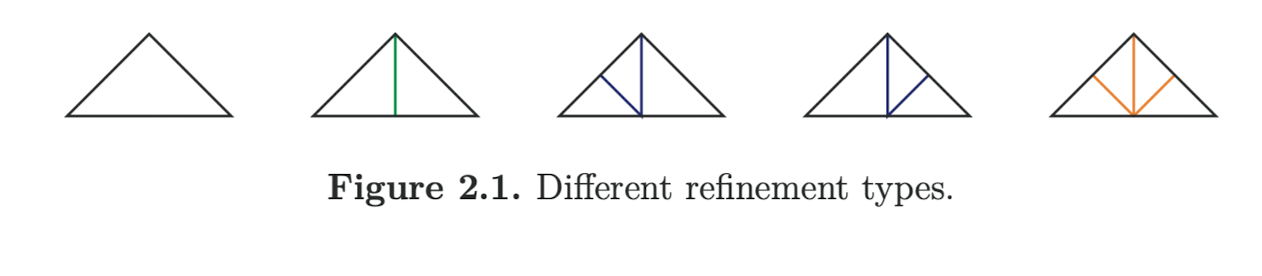
\includegraphics[width = \textwidth]{onelevelrefine.png}
	\end{figure}
\end{definition}

\begin{definition}[admissible triangulation]
	Admissible triangulation is the set of all triangulation that are obtained through finite number of successive one-level refinement, i.e., 
	\begin{equation}
		\mathbb{T}(\mathcal{T}_0):= \{\mathcal{T}|\quad \forall T \in \mathcal{T}: T \text{ is obtained through finite number of 1-level refinement} \}. 
	\end{equation}
\end{definition}

\begin{definition}[admissible triangles]
	The admissible triangles are triangles in the regular triangulation, i.e., 
	\begin{equation}
		\cup \mathbb{T}:= \{ T \in \mathcal{T}: \mathcal{T} \in \mathbb{T}(\mathcal{T}_0) \}.
	\end{equation}
\end{definition}

\begin{definition}[level of a triangle]
	Given $T \in \cup \mathbb{T}$, we define the level of a triangulation as:
	\begin{equation}
		l(T):= \log_2\bigg(\frac{|K|}{|T|}\bigg),
	\end{equation}
	where $K \in \mathcal{T}_0$. 
\end{definition}


\begin{proposition}[elementary properties]
Given $\mathcal{T}_0$ a regular triangulation satisfies the \textbf{(IC)}, we have 
\begin{enumerate}
	\item $\forall T \in \cup \mathbb{T} \exists! K \in \mathcal{T}_0, l(T) \in \mathbb{N}_0$
	\begin{align*}
		|K| = 2^{l(T)} |T|. 
	\end{align*}
	\item Any admissible triangle $T$ is generated by a sequence of length $l(T)$ of the admissible triangles. The sequence is generated by bisection.
	\item There exists at most $|\mathcal{T}_0| \times 8$ interior angles in $\cup \mathbb{T}$. 
	\item Given $T_1, T_2 \in \cup \mathbb{T}$, if $\interior( T_1) \cap \interior( T_2) \neq \emptyset$ and $l(T_1) \le l(T_2)$, then
	\begin{align*}
		T_2 \subset T_1.
	\end{align*}
	\item Given $K \in \bigcup \mathbb{T}$, define the refinement of $K$ w.r.t. the admissible triangulation $\mathcal{T}$:
	\begin{equation}
		\mathcal{T}(K):= \{ T \in \mathcal{T}  | \quad T \subsetneqq K \}.
	\end{equation}
	Then $\mathcal{T}(K)$ is either empty or a regular triangulation.
\end{enumerate}
\end{proposition}


\begin{lemma}[level of triangle by refinement edge]
	Given $\mathcal{T}_0$ the initial triangulation satisfying \textbf{(IC)} and $T_1, T_2 \in \mathcal{T} \in \mathbb{T}$ neighbouring triangles in the sense that
	\begin{align*}
		T_1 \cap T_2 = \{E\}.
	\end{align*}
	Then there 4 cases:
	\begin{enumerate}
		\item $\refine(T_1) \neq E = \refine(T_2)$ 
		\item $\refine(T_1) = E \neq \refine(T_2)$
		\item $\refine(T_1) = E = \refine(T_2)$
		\item $\refine(T_1) \neq E \neq \refine(T_2)$
	\end{enumerate}
\end{lemma}



\subsection{Overlay}
\begin{definition}[Overlay]
  Given $\mathcal{T}_1, \mathcal{T}_2 \in \mathbb{T}$ admissible triangulations, we define the \textbf{overlay}
  \begin{equation}
  	\mathcal{T}_1 \oplus \mathcal{T}_2 := \{ T_1 \cap T_2 | \quad T_1 \in \mathcal{T}_1, T_2 \in \mathcal{T}_2 \text{ with } \interior(T_1) \cap \interior(T_2) \neq \emptyset \}.  
  \end{equation}
\end{definition}
\begin{remark}
Is overlay a triangulation, or even an admissible triangulation?	
\end{remark}

\begin{proposition}[Overlays are admissible]
	Given $\mathcal{T}_1$, $\mathcal{T}_2$ admissible triangulations, then $\mathcal{T}_1 \oplus \mathcal{T}_2$ is admissible and it holds
	\begin{equation}
		|\mathcal{T}_1 \oplus \mathcal{T}_2| + |\mathcal{T}_0| \le |\mathcal{T}_1| + |\mathcal{T}_2|. 
	\end{equation}
\end{proposition}
\begin{proof}
\quad\\
\textbf{1.}:It holds
\begin{equation}
	\bigcup (\mathcal{T}_1 \oplus \mathcal{T}_2) = \overline{\Omega}
\end{equation}
'$\subset$': $\forall T \in \mathcal{T}_1 \oplus \mathcal{T}_2$, since $T = T_1 \cap T_2$ with $\interior(T_1) \cap \interior(T_2) \neq \emptyset$, by the lemma we know either $T_1 \subset T_2$ or $T_2 \subset T_1$, hence 
\begin{align*}
	T \in \mathcal{T}_1 \cup \mathcal{T}_2
\end{align*}
\qquad\\
'$\supset$': $\forall x \in \overline{\Omega}\backslash \mathcal{E}_1 \cup \mathcal{E}_2$, it holds $x \in \interior(T_1) \cap \interior(T_2)$ for some $T_1 \subset \mathcal{T}_1, T_2 \subset \mathcal{T}_2$, hence $T := T_1 \cap T_2 \in \mathcal{T}_1 \oplus \mathcal{T}_2$. 
\begin{align*}
	x \in T \in \mathcal{T}_1 \oplus \mathcal{T}_2. 
\end{align*}

\quad\\
\textbf{2.}: It holds
\begin{equation}
	\forall T, \hat{T} \in \mathcal{T}_1 \oplus \mathcal{T}_2 \text{ with }\interior(T) \cap \interior(\hat{T}) \neq \emptyset:   T = \hat{T}. 
\end{equation} 
\quad\\
\textbf{3.} It holds, $\forall T_1, T_2 \in \mathcal{T}_1 \oplus \mathcal{T}_2$ distinct with nonempty intersection:
\begin{equation}
	 T \cap \hat{T} = \mathcal{V}(T) \cap \mathcal{V}(\hat{T}) \text{ or } T_1 \cap T_2 = \mathcal{E}(T) \cap \mathcal{E}(\hat{T}).
\end{equation}
The nonempty intersection of the interior in the definition of overlay ensures that it belongs to at least one of the regular triangulation. \par 
For $T_1, T_2 \in \mathcal{T}_j$, $j= 1, 2$, the result is trivial since $\mathcal{T}_j$ is a regular triangulation. \par 
For $T_1 \in \mathcal{T}_1 \backslash \mathcal{T}_2, T_2 \in \mathcal{T}_2 \backslash \mathcal{T}_1$, by the lemma of elementary property we have 
\begin{align*}
	T_1 \subsetneqq K_2 \in \mathcal{T}_2 \text{ and } T_2 \subsetneqq K_1 \in \mathcal{T}_1.
\end{align*}
we have
\begin{align*}
	\emptyset \neq \bigg(T_1 \cap T_2 \bigg) \subset \bigg( T_1 \cap K_1 \bigg)\\
	\emptyset \neq \bigg(T_1 \cap T_2 \bigg) \subset \bigg( K_2 \cap T_2 \bigg)
\end{align*}
Since now $T_j, K_j \in \mathcal{T}_j$ for $ j = 1, 2$, we separate the following cases:\par 
Case 1: $K_j \cap T_j = \{z\}$ for any $j$. Then $T_1 \cap T_2 = \{z\}$. \par 
Case 2: $K_j \cap T_j = E_j$. By the lemma of neighbouring triangles we have
\begin{align*}
	l(T_1)  \le l(K_1) + 1 \le l(T_2) \le l(K_2) + 1 \le l(T_1)
\end{align*}
\end{proof}



\subsection{Refine}
If the bisection generates a new triangle, how do we define the refinement edge?
\begin{definition}[neighbour map]
	Given $\mathcal{T}$ an admissible triangulation, we define the map $N: \mathcal{T} \longrightarrow \mathcal{T}$:
	\begin{equation}
	N(T) = 
	\left\{
	\begin{aligned}
		& K  & \refine(T) = \mathcal{E}(K) \text{ with } K \in \mathcal{T} \backslash T \\
		& T  & \refine(T) \subset \partial \overline{\Omega}
	\end{aligned}
	\right.
	\end{equation}
	The neighbouring map finds either the triangle itself or the neighbour along the refinement edge.
\end{definition}

\begin{algorithm}[\text{refine}$(\mathcal{T}, M)$]\label{ALGO_refine}
The algorithm \text{refine(M, $\mathcal{T}$}) takes the $M \in \mathcal{T}$ and compute the coarsest triangulation such that $M$ is refined. 
\begin{algorithmic}
\State $T_0 = M$, \text{bisec}($T_0$), 
\State $T_1 = N(M)$
\State $J = 0$
\For{j = 1, \dots,}	

\State $\{T_{j1}, T_{j2}\} = \text{bisec}(T_j)$
\State $\mathcal{T} = \{\mathcal{T} \backslash T_j\} \cup \{T_{j1}, T_{j2}\}$
\State $T_{j + 1} = N(T_j)$
\If{$\refine(T_{j -1}) = \refine(T_{jk})$}
\State \text{bisec}$(T_{jk})$ 
\EndIf
\If{$T_{j +1} \in \{T_0, \dots, T_j\}$}
\State $J = j$
\text{break}
\EndIf
\EndFor
\end{algorithmic}
\end{algorithm}
\begin{figure}[h]
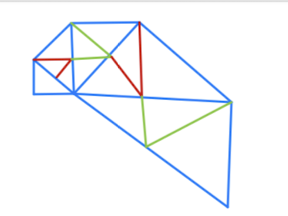
\includegraphics{algo1.png}
\end{figure}

\begin{theorem}[The minimal property of \text{refine}($\mathcal{M, T})$]
We define $\hat{\mathcal{T}}$ as the \textbf{admissible refinement} of a triangulation $\mathcal{T}$ if 
	\begin{equation}
		\forall K \in \mathcal{T}: \hat{\mathcal{T}}(K) \text{ regular triangulation.}
	\end{equation}
It holds
\begin{enumerate}
	\item $\tilde{\mathcal{T}} = \text{refine}(\mathcal{T}, M)$ is a regular triangulation produced by finite many one-level refinement, with $M \in \mathcal{T} \backslash \tilde{\mathcal{T}}$. 
	\item $\tilde{\mathcal{T}} = \text{refine}(\mathcal{T}, M)$ is the coarsest refinement of $\mathcal{T}$ such that $M$ is refined, coarsest in the sense that
		\begin{equation}
		\forall \tilde{\mathcal{T}} \text{ refinement of } \mathcal{T} \text{ w.r.t.$M$}: \mathcal{V}(\hat{\mathcal{T}}) \subset \mathcal{V}(\tilde{\mathcal{T}}). 
	\end{equation}
\end{enumerate}
\end{theorem}
\begin{proof}
\quad\\
\textbf{I: The admissible triangulation:}\\
\textbf{1.} Because $T_0, \dots, T_J$ are pairwise disjoint by design, the algorithm terminates after at most $|\mathcal{T}|$ steps. The termination criteria can be summarised into 2 cases:
\begin{enumerate}
	\item $N(T_{J}) = T_{J-1}$ and $\refine(T_J) = \refine(T_{J -1})$: $l(T_J) = l(T_{J -1}) = l(M) - J + 1 $
	\item $N(T_{J}) = T_J $ and $\refine(T_J) \subset \partial\Omega$: $\forall j = 1, \dots, J$: $l(T_j) = l(M) - j$. 
	\end{enumerate}
\textbf{2.} The generated triangulation is admissible since it's generated by successive one-level refinement defined in the algorithm. We have
\begin{equation*}
	\hat{\mathcal{T}} = \mathcal{T} \backslash \{T_0, \dots, T_J\} \cup\bigg( \bigcup_{j = 0}^J \hat{\mathcal{T}}(T_j)\bigg),
\end{equation*}  
with the nodes
\begin{equation}
	\hat{\mathcal{N}} = \mathcal{N} \cup \{ \text{mid}(E_0) \dots \text{mid}(E_{J + \alpha})\},
\end{equation}
with $\alpha = 0$ in the 1st case and $\alpha = 1$ in the 2nd case. 
\qquad\\
\textbf{II. The minimal property:}
Given $\tilde{\mathcal{T}}$ any admissible refinement of $\mathcal{T}$ w.r.t. $M$, $\hat{\mathcal{T}} = \text{refine}(\mathcal{T}, M)$, we want to show:
\begin{align*}
	\hat{\mathcal{V}}\subset \tilde{\mathcal{V}}. 
\end{align*}  
Prove by mathematical induction. Assume $\{T_0, T_1, \dots, T_J\}$ are the sequence of triangle marked in the refine algorithm and $E_j = \text{Ref}(T_j)$ the corresponding refinement edge. We have as the initial step:
\begin{equation}
	\text{mid}(E_0) \in \tilde{\mathcal{V}}.
\end{equation}
Assume for $j = 0, \dots, J -1$ that
\begin{equation}
	\text{mid}(E_j) \in \tilde{\mathcal{V}},
\end{equation}
then by construction we have
\begin{align*}
	\text{mid}(E_{j + 1}) \in \tilde{\mathcal{V}},
\end{align*}
to avoid the hanging nodes. 
\end{proof}

\begin{theorem}[The refinement commutes]
	Given $M_1, M_2 \in \mathcal{T}$, we have
	\begin{equation}
		\text{refine}( \text{refine}(\mathcal{T}, M_1), M_2) = \text{refine}(\mathcal{T}, M_1) \oplus \text{refine}(\mathcal{T}, M_2).
	\end{equation}
	Hence we may define the refinement of $\mathcal{T}$ over a set of sets $\mathcal{M}$:
	\begin{equation}
		\text{refine}(\mathcal{T}, \mathcal{M}):= \bigoplus_{M \in \mathcal{M}} \text{refine}(\mathcal{T}, M). 
	\end{equation}
\end{theorem}
\begin{proof}
We prove
\begin{equation}
	\mathcal{V}_{12} = \mathcal{V}_{21} = \mathcal{V}_1 \cup \mathcal{V}_2.
\end{equation}
	
\end{proof}



\subsection{Finer Triangulation}
\begin{theorem}[characterisation of the finer relation]
$\forall \mathcal{T}, \hat{\mathcal{T}} \in \mathbb{T}$, the following statements are equivalent.
\begin{enumerate}
	\item $\hat{\mathcal{T}}$ is admissible refinement of $\mathcal{T}$. i.e., $\hat{\mathcal{T}}$ is generated by successive one-level refinement of $\mathcal{T}$. 
	\item $\forall T \in \hat{\mathcal{T}} \exists K \subset \mathcal{T}: T \subset K$. 
	\item $\mathcal{V}(\mathcal{T}) \subsetneqq \mathcal{V}(\tilde{\mathcal{T}}$). 
\end{enumerate}
\end{theorem}
\begin{proof}\quad\\
\textbf{1) $\Rightarrow$ 2):} Given $T \in \hat{\mathcal{T}}$, since $\hat{\mathcal{T}}$ is the finer triangulation, we have
\begin{align*}
	\interior(T) \notin \mathcal{E}(\mathcal{T}). 
\end{align*}
Therefore there exists $K \in \mathcal{T}$, such that
\begin{align*}
	\interior(T) \cap \interior(K) \neq \emptyset \text{ and } l(T) \ge l(K).
\end{align*}
By the elementary property of the admissible triangulation we have
\begin{align*}
	T \subset K. 
\end{align*}
\quad\\
\textbf{2) $\Rightarrow$ 3)}: Assuming there exists $z \in \mathcal{V} \backslash \hat{\mathcal{V}}$, discuss the case where $z$ in different kind of refine edge 
\qquad\\
\textbf{3) $\Rightarrow$ 1)}: Assume $\mathcal{T}_j, j = 1, \dots, J$ are generated by refinement by nodes, then:
\begin{equation}
	\forall T \in \hat{\mathcal{T}} \exists K \in \mathcal{T}_j: T \subset K. 
\end{equation}
For $j = 1$, by \textbf{2)} we find $M_1$ and  $\mathcal{T}_2 = \text{refine}(\mathcal{T}_1, M_1)$. 
\end{proof}


\begin{definition}[finer triangulation]
		
\end{definition}
	

\begin{algorithm}[refinement by nodes]
\begin{algorithmic}
\State $\mathcal{T}_1 = \mathcal{T}$. 
\For{j = 1, \dots}
\If{$\hat{\mathcal{V}} \backslash \mathcal{V}_j = \emptyset$}
\State $J = j$,  \text{break}
\Else 
\State \text{choose } $z \in \hat{\mathcal{V}} \backslash \mathcal{V}_j$ 
\State \text{choose } $T$ with $z \in \mathcal{V}(T)$
\State \text{choose } $M_j \in \hat{\mathcal{T}}_j$: $T \subset M_j$. 
\State $\mathcal{T}_{j + 1} = \text{refine}(\mathcal{T}_j, M_j)$. 
\EndIf	
\EndFor
\end{algorithmic}
\end{algorithm}
\quad\\
\textbf{Question:} Why can we choose $M_j$ as such. 
\begin{equation}
	\forall T \in \hat{T} \exists K \in \mathcal{T}_j: T \subset K
\end{equation}





\subsection{Overhead Control}
In this section we assume that $\mathcal{T}_0$ with \textbf{IC} and the sequence of regular triangulation
	\begin{align*}
		\mathcal{T}_{1}, \dots, \mathcal{T}_L \in \mathbb{T}, \qquad \mathcal{M}_l \subset \mathcal{T}_l
	\end{align*}
	is generated by the refine algorithm:
	\begin{align*}
		\mathcal{T}_{l + 1} = \text{refine}(\mathcal{T}_l, \mathcal{M}_l), \quad l = 0, \dots, L -1.
	\end{align*}
This section we prove that, in the (local) mesh refinement,  the number of triangles needed is controlled by some a priori global constant, i.e., 
\begin{align*}
	|\mathcal{T}_L| - |\mathcal{T}_0| \le C_{BVD} \sum_{l = 0}^L |\mathcal{M}_l|.
\end{align*} 
\quad\\
First we introduce 2 constant, before that we define the distance and diameter in a triangulation:
\begin{definition}
	Given $A, B, C \subset \mathbb{R}^2$, we define
	\begin{enumerate}
		\item \text{distance:} $\dist(A, B) := \inf_{a \in A, b \in B} |a - b|,$
		\item \text{diameter:} $\diam (C):= \sup_{c_1, c_2 \in C} |c_1 - c_2|$. 
	\end{enumerate}
\end{definition}
\begin{definition}[two global constant]
\begin{equation}
	d: = \min_{T \in \mathcal{T}_0} |K|, \quad D:= \max_{\mathcal{T} \in \mathbb{T}}\max_{T \in \mathcal{T}} \diam(T) 2^{\frac{l(T)}{2}}
\end{equation}
\end{definition}
\begin{remark}
	$D$ is close related to the area and level relation in a triangulation, we have in a reference triangle
	\begin{align*}
		\bigg( \diam(T) 2^{\frac{l(T)}{2}} \bigg)^2 = 4|T| 2^{l(T)} = 4 |K|,
	\end{align*}
	where $K \in \mathcal{T}_0$
\end{remark}


\begin{lemma}
	Given $M \in \mathcal{T} \in \mathbb{T}$, then for any $T \in \text{refine}(M, \mathcal{T}) \backslash \mathcal{T} $ generated in the process, we have
	\begin{enumerate}
		\item $\text{level control: }l(T) \le l(M) + 1$
		\item $\text{distance control: }\dist(M, T) \le D 2^{\frac{3 - l(T)}{2}}$
	\end{enumerate}
\end{lemma}
\begin{proof}
\quad\\
\textbf{I. For the statement of the level:}\\
By the refinement algorithm \eqref{ALGO_refine} we observe
\begin{align*}
	 \underbrace{T_0}_{:= M},\quad T_1, \dots, T_J. 
\end{align*}
Given any $T \in \text{refine}(\mathcal{T}, M)$, assume $T  \subsetneqq T_m$ with $m \in \{0, \dots, J\} $, then\\
\textbf{Case 1:} $m = 0$. 
Trivial and we have 
\begin{align*}
	l(T) = l(M) + 1
\end{align*}
\textbf{Case 2:} $m \in \{1, \dots, J -1\}$, in each one-level refinement the level is increased at least by 1. Define $k:= l(T) - l(T_m)$, we have for $k = 1$ the green refinement and $k = 2$ the blue refinement. By proof in the minimal property we have
\begin{align*}
	l(T) = l(T_m) + k  =  l(M) - m + k \le l(M) + 1 . 
\end{align*}
\textbf{Case3:} $m = J$. Again in the proof of the minimal property we separated 2 cases:
\begin{align*}
	l(T_J) = l(T_{J -1}) \text{ and } l(T_J) = l(T_{J -1}) -1. 
\end{align*}
We have
\begin{align*}
	& l(T) = l(T_J) + 1 = l(M)-J+1+1 \le l(M) + 1\\
	& \text{and}\\
	& l(T) = l(T_J) + k = l(M) - J + k\le l(M) + 1. 
\end{align*}
\quad\\
\textbf{II. For the bound of distance.}
By construction we know for $j \in \{1, \dots, J -1\}$, 
$T_{j -1}, T_{j +1}$ share a vertex and therefore
\begin{align*}
	\dist(T_{j -1}, T_{j+1}) = 0 \quad \text{for} j = 1, \dots, J -1.
\end{align*}
Define $T_m$ that generates $T$ with one blue(green) refinement, we have $\dist(T, T_{m -1}) =0$, hence
\begin{align*}
	\dist(T, M) &\le \dist(T, T_{m-1}) + \diam(T_{m-1}) + \dist(T_{m -1}, M)\\
	& \le 0 + \diam(T_{m -1}) + \diam(T_{m -3})  + \dist(T_{m -3}, M)\\
	& \dots \\
	& \le \sum_{j = 1}^{\lfloor \frac{m}{2} \rfloor} \diam(T_{m - 2j + 1})\\
	&  \le \sum D 2^{-\frac{l(T) - 2j - 3}{2}} \\
	& \le D 2^{\frac{3 - l(T)}{2}} \sum_{k = 1}^\infty 2^{-k}\\
	& = D 2^{\frac{3 - l(T)}{2}}
\end{align*}
\end{proof}

We need a generic measure function that converges w.r.t. $T$ as the marked triangles increases. The level is the clear choice. 
\begin{definition}[The measure function]
For the $L$ times refinement $\mathcal{T}_L$ we define $\mathcal{M}:= \mathcal{M}_0 \cup \mathcal{M}_1 \dots \mathcal{M}_{L -1}$ and the measure function
\begin{align*}
	\lambda: (\bigcup_{j = 1}^L \mathcal{T}_j) \times \mathcal{M} \rightarrow [0, \sqrt{2}],
\end{align*}
with
\begin{equation}
\lambda(T, M) =  \left\{
	\begin{aligned}
		& 2^{\frac{l(T) - l(M)}{2}}  & l(T) \le l(M) + 1 \text{ or } \dist (T, M) \le D 2^{ \frac{5 - l(T)}{2}}. \\
		& 0 &\text{else}.
	\end{aligned}
	\right.
\end{equation}
\end{definition}

\begin{lemma}[a lower bound]
For any $T \in T_L \backslash T_0$, it satisfies
\begin{equation}
	\frac{1}{1 + 2^{- \frac{3}{2}}} \le \sum_{M \in \mathcal{M}} \lambda(T, M).
\end{equation}
\end{lemma}
\begin{proof}
Since $T \notin \mathcal{T}_0$, there exists $j(1) \in \{0, L -1\}$, such that
\begin{align*}
	T = \text{refine}(\mathcal{T}_{j(1)}, M_{j(1)})
\end{align*} 
Run algorithm to get successively the sequence, for given $(\mathcal{T}_{j(\kappa)}, M_{j(\kappa)})$
\begin{align*}
	& \text{find }(\mathcal{T}_{j(\kappa + 1)}, M_{j(\kappa + 1)}) \text{ s.t. }  M_{j(\kappa)} \in \text{refine}(\mathcal{T}_{j(\kappa + 1)}, M_{j(\kappa + 1)})\\
	& \text{stops with } \kappa = k \text{ if} \\
	&M_{j(\kappa)} \in \mathcal{T}_0 \text{ or } \lambda(T, M_{j(\kappa)}) = 0. 
\end{align*}
This algorithm always stops since 



\quad\\
\textbf{Case1:}  $M_{j(k)} \in \mathcal{T}_0$. In this case we reach The case implies $\lambda(T, M_{j(k)}) > 0$, hence
\begin{align*}
	\sum_{M \in \mathcal{M}} \lambda(T, M) \ge \lambda(T, M_{j(k)}) = 2^{(l(T) - 0)\slash 2}  = \sqrt{2}.
\end{align*}
\qquad\\
\textbf{Case2:} $\dist(M_{j(k)}, T) \ge \frac{5 - l(T)}{2}$.
\end{proof}

\begin{lemma}[a upper bound]
	For any $M \in \mathcal{M}:$
	\begin{equation}
		\sum_{T \in \mathcal{T}_L \backslash \mathcal{T}_0} \lambda(T, M) \le \frac{2}{\sqrt{2} -1 } \pi D^2 (1 + 2^{\frac{5}{2}})^2 d^{-1}
	\end{equation}
\end{lemma}


\begin{theorem}
	There exits a generic constant (sorely depends on $\mathcal{T}_0$) $C_{BDV}$, such that 
	\begin{equation}
		|\mathcal{T}_L| - |\mathcal{T}_0| \le C_{BDV} \sum_{l = 0}^{L -1} |\mathcal{M}_l|.
	\end{equation}
	with $C_{BDV}(\mathcal{T}_0) \approx 5000$.
\end{theorem}
\begin{proof}
	Observe $|\mathcal{T}_L \backslash \mathcal{T}_0|$, multiplied both sides with the lower bound of $\sum_{M \in \mathcal{M}} \lambda(T, M)$, defined as $L$, and define the upper bound of $\sum_{T \in \mathcal{T}_L \backslash \mathcal{T}_0} \lambda (T, M) $ as $U$, we have
	\begin{align*}
		L |\mathcal{T}_L \backslash \mathcal{T}_0| &\le L \sum_{T \in \mathcal{T}_L \backslash \mathcal{T}_0} 1 \\
		& \le \sum_{T \in \mathcal{T}_L \backslash \mathcal{T}_0} \sum_{M \in \mathcal{M}} \lambda(T, M)\\
		& \le  \sum_{M \in \mathcal{M}} \sum_{T \in \mathcal{T}_L \backslash \mathcal{T}_0} \lambda(T, M)\\
		& \le \sum_{M \in \mathcal{M}} U\\
		& = U|\mathcal{M}|. 
	\end{align*}
\end{proof}



\section{Discrete Analysis and PMP}
In this section we investigate various aspect of analysis in the broken polynomial space on the domain of regular triangulation.
\subsection{The Convex Regularity}
\begin{theorem}[The Convex Regularity]
	Given $\Omega$ a \textbf{convex} Lipschitz domain and $f \in L^2(\Omega)$, the \textbf{PMP} satisfies
	\begin{equation}
		\|D^2 u \|_{L^2(\Omega)}^2 \le \|f\|_{L^2(\Omega)}^2
	\end{equation}
\end{theorem}
\begin{proof}
\end{proof}

\begin{example}[Non-convex domain](By Micheal Randy). 

\qed
\end{example}

The example above illustrate that singular solution may appear on the non-convex domain. We observe the sector domain defined as:
\begin{equation}
	\omega_j:= \{( r, \varphi_j + \varphi): 0 < \varphi < \omega_j, 0 < r < 1 \}. 
\end{equation}
 We observe that singular solution may depend on $\omega_j$, in fact, any changes on the boundary condition may cause changes in the singular solution. We allow the now 2 types of changes on the boundary:
 \begin{enumerate}
 	\item changes of the boundary type.
 	\item changes on the vertex. 
 \end{enumerate}

Depending on the changes of the boundary we get the \textbf{stress intensity factor}
\begin{equation}
	\alpha_{jk} = \left\{
	\begin{aligned}
		& \frac{k\pi}{\omega_j} &\text{if there is no change on the boundary}, \\
		& \frac{(k - \frac{1}{2}) \pi }{\omega_j} & \text{if there is some change on the boundary}
	\end{aligned}
	\right.
\end{equation}

\begin{theorem}[the decomposition theorem]
	Given $\Omega \subset \mathbb{R}^2$ with polygon boundary $\Gamma$ defined by $P_1, \dots, P_J$ with $\Gamma_j = \conv(P_j, P_{j + 1})$ and $\Gamma = \cup_{j = 1}^{J -1} \Gamma_j$.\par 
	Suppose the boundary condition changes \textbf{only} at $P_1, \dots, P_J$.  The Dirichlet boundary is denoted by $\Gamma_D$ and the Neumann boundary is denoted by $\Gamma_N:= \Gamma \backslash \Gamma_D$. Observe the Mixed Poisson Problem for $s > 0$ :
	\begin{equation}
	\begin{aligned}
		\textbf{(MPMP)} \quad
		& - \Delta u = f \in H^{s - 1}(\Omega),\\
		& \partial_\nu u = g \in H^{s - \frac{1}{2}}(\Gamma_j) \text{ on } \Gamma_j \subset \bar{\Gamma},\\
		& u = 0 \text{ on } \Gamma_D,
	\end{aligned}
	\end{equation}
	which admits a solution in 
	\begin{equation}
		H^1_D(\Omega):= \{ u \in H^1(\Omega)|\quad u_{\Gamma_D} \equiv 0 \}.
	\end{equation}
	Then there exists coefficients $\alpha_{jk}$, such that
	\begin{equation}
		u -  \sum_{j = 1}^J \sum_{\substack{k = 1\\ \alpha_{jk} < s}}^\infty S_{jk} \chi_{j} \in H^{1 + s}(\Omega).
	\end{equation} 
\end{theorem}



\subsection{PF Inequality \& Quasi-Interpolation}
\subsubsection{Friedrich's inequality}
\begin{theorem}
	Given $\Omega$ a bounded Lipschitz domain, $f  \in W^{1, p}(\Omega)$, if there exits $\Sigma \subset \partial\Omega$ such that 
	\begin{align*}
		\int_\Sigma f dS = 0. 
	\end{align*}
	Then there exists a constant $C$ such that 
	\begin{align*}
		\|f\|_{L^p} \le C \|\nabla f\|_{L^p}. 
	\end{align*}
\end{theorem}


In the following we investigate the Poincare-Friedrich inequality in the discrete form. 
\begin{theorem}[Payne-Weinberg(1962)]
	Given $\Omega \subset \mathbb{R}^n$ \textbf{convex} open domain and we denote
	\begin{align*}
		\diam(\Omega):= \text{diameter of }\Omega,
	\end{align*}
	then we have
	\begin{equation}
		\sup_{f \in H^1(\Omega) \cap L_0^2(\Omega)} \frac{\|f\|_{L^2}}{||| f|||} = C_p = \frac{\diam(\Omega)}{\pi}.
	\end{equation}
	This diameter is sharp without further information. 
\end{theorem}


With Payne-Weinberger as the guidance, we investigate the Poincare constant with different $\Omega$, in particular in the case of the triangulation. 


\begin{theorem}[Poincare Inequality on equilateral triangles]
	On a equilateral triangle we haven for all $f \in H^1_0(\Omega)$:
	\begin{align*}
		C_{PW} = \frac{\diam(\Omega)}{j_{1, 1}},
	\end{align*}
	where $j_{1, 1} > \pi $ is the smallest positive \textbf{root of the Bessel function of the first kind}.
\end{theorem}

\begin{theorem}[Poincare Inequality on triangles]
	On a triangle $T$ it holds for all $f \in H^1_0(\Omega)$:
	\begin{align*}
		\|f\|_{L^2(T)} \le C_{PW} \|\nabla f\|_{L^2(T)}
	\end{align*}
	with 
	\begin{align*}
		C_{PW} \le \frac{\diam}{j_{1,1}}.
	\end{align*} 
\end{theorem}
\begin{remark}
It can be written in general
\begin{align*}
	\|f\|_{L^2(T)} \le C_{PF} h_T |||f|||.
\end{align*}	
\end{remark}

\begin{proof}
	The computer experiment proves the worst case Poincare constant is provided by the equilateral triangles. 
\end{proof}

 
\begin{theorem}[Poincare Inequality on a patch]
	For any (closed) patch $w_z \in \mathcal{N}(\Omega)$ and define the Sobolev function space on a patch:
	\begin{equation}
		H^1(\mathcal{T}(z)):= \{f \in L^2(w_z): \quad \forall T \in \mathcal{T}(z): f|_{\interior(T)} \in H^1(\interior(T)),
	\end{equation}
	with \textbf{zero jump condition:}
	\begin{equation}
		f \in H^1(\mathcal{T}(z)):  \int_E [f]_E ds = 0 \quad \forall E \in \mathcal{E}(z),
	\end{equation}
	then for all $J:= |\mathcal{T}(z)|$ and $\bar{f} \in \mathbb{R}$ such that
	\begin{equation*}
		\min_{T \in \mathcal{T}(z)} \int_T (f - \bar{f}) dx \le 0 \le \max_{T \in \mathcal{T}(z)} \int_T (f - \bar{f}) dx, 
	\end{equation*}
	we have
	\begin{equation}
		\|f - \bar{f}\|_{L^2(w_z)}^2 \le \bigg(\frac{1}{j_{1,1}} + \frac{\max_{T \in \mathcal{T}(z)}|T| }{4(1 - \cos(\frac{\pi}{J})) \min_{T \in \mathcal{T}(z)}|T|}\bigg) \|h_\mathcal{T} \nabla f\|_{L^2(w_z)}^2 
	\end{equation}
\end{theorem}
\begin{remark}
As before, the Poincare inequality on a patch can be written as 
\begin{align*}
	\|f\|_{L^2(w_z)} \le C_{PF}(w_z) h_T |||f|||_{w_z}. 
\end{align*}	
\end{remark}


\subsubsection{The quasi interpolation}
\begin{definition}[the quasi-interpolation]
	Given $\mathcal{T} \in \mathbb{T}, \hat{\mathcal{T}} \in \mathbb{T}(\mathcal{T}), \hat{v} \in \hat{\mathcal{T}}$, for $z \in \mathcal{V}(\mathcal{T})$ and $w_z = \mathcal{T}(z)$, define the quasi-interpolation
	\begin{equation}
		v(z) = \left\{
		\begin{aligned}
			& 0 \quad & z \in \partial\Omega,\\
			&\fint_{w_z} \hat{v} \quad & \mathcal{T}(z) \cap \hat{\mathcal{T}}(z) = \emptyset,\\
			& \hat{v} \quad & \mathcal{T}(z) \cap \hat{\mathcal{T}}(z)  \neq \emptyset. 
		\end{aligned}
		\right.
	\end{equation}
\end{definition}

\begin{theorem}
	The quasi-interpolation admits the discrete reliability, i.e., 
	\begin{enumerate}
		\item $v = \hat{v}$ on $\mathcal{T} \cap \hat{\mathcal{T}}$. 
		\item $\|h_\mathcal{T}^{-1}( \hat{v} - v)\|_{L^2(\Omega)} + ||| v|||_{\Omega} \le C_{QI} |||\hat{v}|||_\Omega,$
	\end{enumerate}
	where the constant $C_{dQI}$ depends on $\omega_0$. 
\end{theorem}
\begin{proof}\quad\\
\textbf{ad1: nodal PF control.} claim: $\|\hat{v} - v(z)\|_{L^2(\omega_z)} \le C h_T|||v|||_{w_z}$. \\
case1: $\mathcal{T}(z) \cap \hat{\mathcal{T}}(z) = \emptyset$. Since the boundary contains no jump it holds by Poincar\'e's inequality that 
\begin{align*}
	\|\hat{v} - v(z)\|_{w_z} = \|\hat{v} - \fint_{w_z} \hat{v}\|_{w_z} \le h_T C_P ||| \hat{v}|||.
\end{align*}
case2: $z \in \partial\Omega$, let $\Sigma$ boundary edge of $w_z$, it hold $\int_\Sigma \hat{v} = 0$, apply Friedrich's inequality we have
\begin{align*}
	\|\hat{v} - v(z)\|_{w_z} = \|\hat{v}\|_{w_z} \le h_T C_F |||\hat{v}|||.
\end{align*}
case3: $\exists T \in \mathcal{T}(z) \cap \hat{\mathcal{T}}(z)$, $\forall \hat{z} \in \mathcal{V}(T)$ it holds $v(\hat{z}) = \hat{v}(\hat{z})$, hence on $T$ $v = \hat{v}$. Apply again the Friedrich's inequality we have
\begin{align*}
	\|\hat{v} - v \|_{w_z} \le h_T C_F(w_z \backslash T) |||\hat{v} - v|||_{w_z}.
\end{align*}
However that is not the claim. Now define 
\begin{align*}
	w:= \hat{v} - v(z), \quad w_T:= \fint_T \hat{v}, \quad \bar{w}:= \fint_{w_z} \hat{v},
\end{align*}
Since $w \in S_0^1$ and vanish on $z$, we can apply Friedrich:
\begin{align*}
	\|w\|_{w_z} \le C(w_z) |||w||| \le |||\hat{v}|||
\end{align*}

\quad\\
\textbf{ad2: PF control on triangles} claim: $\forall T \in \mathcal{T}, \Omega_T := \interior(\cup_{z \in \mathcal{V} (T)} w_z)$, it holds
\begin{align*}
	\|\hat{v} - v\|_T \le C(T)|||\hat{v}|||_{\Omega_T}. 
\end{align*}
Observe 
\begin{align*}
	\| \hat{v} - v \|_T^2 &= \int_T \sum_{i = 1}^3 |\bigg( \hat{v} - v(z_i) \bigg) \varphi_i|^2 \\
	&\le \int_T \sum_i \bigg(\hat{v} - v(z_i)\bigg)^2 \sum_i \varphi_i^2 \\
	& \le \sum_i \|\hat{v} - v(z_i)\|_T^2 \\
	&\le \sum_i C(T) h_T^2 |||\hat{v}|||_{w_z}^2
\end{align*}

\quad\\
\textbf{ad3: discrete energy control} claim:  there exits $C(\omega_0)$ such that 
\begin{align*}
	|||v|||_T \le C(\omega_0) |||\hat{v}|||_{\Omega_T}
\end{align*}
shape regularity.
\end{proof}




\subsection{Trace and jump control}
\begin{lemma}[The Trace Identity]
	Given $T \subset \mathbb{R}^n$ a triangle and $P$ a vertex with the opposite edge $E$, then it holds
	\begin{equation}
		\fint_E f ds = \fint_T f + \frac{1}{n} \fint_T (x - P) \cdot \nabla f dx.
	\end{equation}
\end{lemma}
\begin{proof}
Define
\begin{align*}
	g(x) := (x - P) f(x).
\end{align*}
Observe
\begin{align*}
	\int_T \div g = \int_{\partial T} g \cdot \nu  = \int_E \langle x - P, \nu \rangle f(x) = \dist(P, E) \int_E f.
\end{align*}
On the other hand 
\begin{align*}
	\int_T \div g = \int_T \langle \nabla f, x - P \rangle + \div(x- P) f(x) = \int_T \langle \nabla f, x - P\rangle + n \int_T f. 
\end{align*}
Taking the integral mean we get the result. 
	
\end{proof}

\begin{lemma}[The Trace Inequality]
	Let $f \in W^{1, 1}(T)$ and $\diam(T) = d$. Then
	\begin{equation}
		\int_E|f|  \le \frac{|E|}{|T|} \int_T |f| + \frac{|E|}{|T|} \frac{d}{n} \int_T |\nabla f|.
	\end{equation}
	From the statement it holds:
	\begin{align*}
		h^{\frac{1}{2}}\|f\|_{L^2(E)} \lessapprox \bigg(  \| f\|_{L^2(T)} + h_T |||f||| \bigg)
	\end{align*}
\end{lemma}
\begin{proof}
Taking $(x - P) \le d$ and get the estimate. 
\end{proof}

Trace inequality and inverse estimate combined provides us with powerful tools to estimate the flux or jumps. We now introduce the \textbf{inverse estimate} of the generally known Poincar\'e inequality. Recall when estimate $L^2$ norm with $H^1$ seminorm, the $H^1$ seminorm is multiplied by the mesh size, in the inverse estimate it's the other way around. \par 
The inverse estimate in general doesn't hold. However in the conforming polynomial space we can compute the inverse estimate by \textbf{shape regularity}.

\begin{lemma}[The inverse estimate]
	$\forall T \in \mathcal{T}  \forall p \in P_k(\mathcal{T})  \exists c_{inv}(\omega_0)$, such that
	\begin{equation}
		|||p||| \le c_{inv}(\omega_0)h_T^{-1} \|p\|_{L^2(T)}. 
	\end{equation}
\end{lemma}
\begin{proof}
	shape regularity.
\end{proof}

\begin{corollary}[discrete jump control]
	$\forall \mathcal{T} \in \mathbb{T} \forall g \in P_k(\mathcal{T})$, it holds
\begin{equation}
	\sqrt{\sum_{K \in \mathcal{T}} |K|^\frac{1}{2} \sum_{E \in \mathcal{E}(K)} \|[g]_E\|_{L^2(E)}^2 } \le \Lambda_1 \|g\|_{L^2(\Omega)}. 
\end{equation}
\end{corollary}





\section{Courant FEM Method}
\subsection{CFEM: the discrete formulation.}
First we define the broken polynomial space the in the conforming scheme, i.e., the Courant finite element $\mathcal{S}^1_0(\mathcal{T})$
\begin{definition}[Courant finite element]
Define the polynomial space on a regular triangulation
\begin{equation}
	P_n(\mathcal{T}):= \{v \in L^\infty:\quad v|_T \in P_n(T)\}.
\end{equation}
	The Courant Finite Element method (CFEM) is a Galerkin scheme with the finite dimensional function space:
\begin{equation}
	S_0^1(\mathcal{T}) \equiv P_1(\mathcal{T}) \cap C_0(\overline{\Omega}), 
\end{equation}
i.e., the space of \textbf{piecewise affine linear} on the triangle  and \textbf{globally continuous function} functions. 
\end{definition}

\begin{lemma}
	It holds $\forall f \in L^2(\Omega)$, 
	\begin{align*}
		\mathbb{R} \perp_{L^2} (f - \Pi_0 f).  
	\end{align*}
\end{lemma}

After establishing the conforming broken polynomial space, we observe the the projection of the exact solution onto the test space, we conclude in the following theorem that the orthogonal projection of the exact solution onto the conforming space is the \textbf{discrete solution}.

\begin{definition}[discrete weak solution]
	Given the PMP, define the \textbf{discrete weak solution} $u_h$ on the conforming space:
	\begin{equation}
		\int_\Omega \nabla u_h \nabla v_h = \int_\Omega f v_h \quad \forall v_h \in \mathcal{S}_0^1(\mathcal{T}). 
	\end{equation}
\end{definition}

\begin{theorem}[best approximation property of the Courant discrete solution]
	 Given PMP and $u$ the exact weak solution, it holds 
	\begin{equation}
		|||e|||: = |||u_h - u ||| = \min_{v_h \in S_0^1}|||u - v_h|||.
	\end{equation}
	i.e.,
	\begin{align*}
		e \perp_{H^1}  S_0^1(\mathcal{T}). 
	\end{align*}
\end{theorem}
\begin{proof}
\quad\\
\textbf{1. $\mathcal{S}_0^1(\mathcal{T}) \subset H_0^1(\Omega)$:} 
\begin{enumerate}
	\item Vanishing Boundary: Trivial.
	\item The weak derivative exists and belongs to $L^2$. we show $\forall v_h \in S_0^1(\Omega) \exists \nabla_{PW} v_h \in L_2:$
	\begin{equation}
	\begin{aligned}
	 \\
	&\int_\Omega v_h \div \varphi + \nabla_{PW} v_h \cdot  \varphi dx = 0 \quad \forall \varphi \in \mathcal{D}(\Omega)^n ,
	\end{aligned}
	\end{equation}
	indeed, 
	\begin{align*}
		\int_\Omega v_h \div \varphi + \nabla_{PW} v_h \varphi dx 
		&= \sum_{j = 1}^N \int_{T_j} v_h\nabla \varphi + \nabla v_h \varphi dx\\
		&=  \sum_{j = 1}^N \int_{\partial T_j} (v_h \varphi) \cdot \nu_E dx\\
		&= \sum_{E \in \mathcal{E}} \int_E (v_h \varphi)(\nu_E - \nu_E) dx \\
		&= 0
	\end{align*}
	Since we have the regular triangulation. 
\end{enumerate} 
\textbf{2. Well-posedness of the discrete problem:}
there exists a unique $u_h \in \mathcal{S}_0^1(\mathcal{T})$, such that
\begin{align*}
	\int_\Omega \nabla u_h \cdot \nabla v_h = \int_\Omega f v_h \qquad \forall v_h \in \mathcal{S}_0^1(\mathcal{T})
\end{align*}
\textbf{3. Well-posedness of the continuous problem:} there exists a unique $u \in H_0^1(\Omega)$, such that
\begin{align*}
	\int_\Omega \nabla u \cdot \nabla v = \int_\Omega f v \qquad \forall v \in H_0^1(\Omega)
\end{align*}
\textbf{4. The best approximation:} to show
\begin{align*}
	e   \perp \mathcal{S}_0^1(\mathcal{T}). 
\end{align*}
\end{proof}




\subsection{Nodal Interpolation}
In this section we observe the conforming interpolation. The nodal interplant is in general not the best approximation in the sense of the discrete solution. However in the conforming case it is and admits a priori estimate. 

\begin{definition}[the nodal interplant]
\begin{equation}
\begin{aligned}
	I: H^2(\Omega) &\rightarrow \mathcal{S}_0^1(\mathcal{T})  \\
	Iu(x) &\mapsto \sum_{z \in \mathcal{V}(\mathcal{T})} u(z) \varphi_z(x).  	
\end{aligned}
\end{equation}
\end{definition}









\subsubsection{Nodal Interpolation Error Estimate}
Objective of this section is to estimate the error bound
\begin{equation}
	||| u - Iu ||| \le C(\mathcal{T}) \| h_{\mathcal{T}}  D^2 u\|_{L^2(\Omega)} \qquad \forall u \in H^2(\Omega)
\end{equation}



\begin{proposition}[Poincare on triangles]
	Let $T$ be the triangle with vertex $P$ and the opposite edge $E$. Let $f \in H^1(T)$ satisfy 
	\begin{align*}
		\int_E f ds = 0. 
	\end{align*} 
	Then it holds
	\begin{equation}
		\|f\|_{L^2(T)} \le \sqrt{\frac{\max_{x \in E} |P - x|^2}{8} + \frac{h_T^2}{j_{1, 1}^2}}|f|_{H^1(T)}.
	\end{equation}
\end{proposition}
\begin{proof}
	By the Cea's lemma we have
	\begin{align*}
		\|f\|_{L^2} = \|f - \fint_T f\|_{L^2} + \|\fint_T f \|_{L^2}.
	\end{align*}
	The first part on the RHS can be estimated by the discrete Poincare Inequality:
	\begin{align*}
		\| f - \fint_T f\|_{L^2} \le \frac{h_T}{j_{1,1}} |f|_{H^1}.
	\end{align*}
	The second part of the RHS can be estimated by the trace inequality
	\begin{align*}
		|\int_T f|^2 &= \frac{1}{2} |\int_T (x - P) \cdot \nabla f|^2\\ 
		&\le \frac{1}{2}\|x - P\|_{L^2}^2 |f|_{H^1}^2\\
		&\le \frac{1}{2} (\frac{\max_{x \in E} |x - P|}{2|T|})|f|_{H^1}^2.
	\end{align*}
\end{proof}

\begin{lemma}
	For $a \in \mathbb{R}^2$, $\tau, \nu \in \mathbb{R}^2$, it holds
	\begin{align*}
		|a|^2 \le \frac{\langle a, \tau \rangle^2 + \langle a, \nu \rangle }{1 - \langle \tau, \nu \rangle}.
	\end{align*}
\end{lemma}


With the Poincar\'e estimate and the geometrical lemma above we prove the a priori estimate of the Courant finite element.
\begin{theorem}[Interpolation Error Estimate for $H^2$ function]
	Given a triangle $T$ with $\diam(T) = h_T$ and largest inner angle $ 0 < \omega < \pi$. Then there exists constant $c(\omega)$ such that for all $v \in H^2(T)$ it satisfies 
	\begin{equation}
		|v - Iv|_{H^m}(T) \le c(\omega) h_T^{2 - m} |v|_{H^2(T)} \quad\text{for }m = 0, 1, 2.
	\end{equation}
	The constants are
	\begin{itemize}
		\item $c_0(\omega) \lesssim 1$.
		\item $c_1(\omega) = \frac{\sqrt{\frac{1}{4} + \frac{2}{j_{1, 1}^2}}}{\sqrt{1 - |\cos(\omega)}|}$.
		\item $c_2(\omega) = 1$. 
	\end{itemize}
\end{theorem}
\begin{proof}
	Proof for the case of $m = 1$, where we have the Poincar\'e energy estimate. Define
	\begin{align*}
		f_j:= \tau_j  \cdot \nabla (v - Iv) \in L^2(T). \text{ with } \tau_j \text{ normal on $E_j$.} 
	\end{align*}
	$f_j$ satisfies $\int_{E_j} f_j = 0$ by definition of nodal interpolation, hence Poincar\'e applicable. It holds
	\begin{align*}
		| v - Iv |_{H^1}^2 &= \int_T \langle \nabla (v - I v), \nabla (v - Iv) \rangle\\
		& \le \int_T \frac{f_1^2 + f_2^2  }{1 - \langle \tau_1, \tau_2 \rangle}.\\
		& \le  c(\omega) ( \|f_1\|^2_T + \|f_2\|_T^2 )\\
		(\text{Poincar\'e})
		& \le c(\omega) h_T^2 (|f_1|_{H^1}^2 + |f_2^2|^2_{H^1})\\
		& \le c(\omega)h_T^2 |v|_{H^2}^2 
	\end{align*}
\end{proof}

\begin{definition}[maximal(minimal) angel condition]
	A family of triangulation $(\mathcal{T}_l)_{l \in \mathcal{L}}$ is said to satisfies the \textbf{maximal(minimal) angle condition} if 
	\begin{align*}
		\forall l \in \mathcal{L} \forall T \in \mathcal{T}_l: \text{ angles of $T$ are bounded above(below) by }0 <  \omega < \pi.  
	\end{align*}
\end{definition}
\begin{remark}
\quad
\begin{enumerate}
	\item Minimal angle condition implies the maximal angle condition. The converse is \textbf{not} true. 
	\item Under the maximal angle condition, we have for $\Omega \subset \mathbb{R}^2$:
	\begin{align*}
		|||u - Iu||| \le C(\Omega) \|h_l D^2 u \|_{L^2(\Omega)}
	\end{align*}
\end{enumerate}	
\end{remark}



\subsection{Local Mesh-refinement}
It is clear from the last section that if $u \in H^2(\Omega)$, we would have
\begin{equation*}
	|||u - u_l||| \lessapprox \|D^2u\|_{L^2(\Omega)} \|h_l\|_\infty.
\end{equation*}
However, for the non-convex domain with re-entering corner, we have the generic singularity. 

\begin{theorem}[Interpolation Error for Singular Functions]\quad\\
\textbf{i).}
\begin{equation}
	\diam(\omega_P)^\alpha \approx |u_s|_{H^1(\omega_P)} \approx |u_s - I_l|_{H^1(\omega_P)} \approx \min_{q \in P_1(T)} |u_s - q|_{H^1(T)} \qquad \forall T \in \mathcal{T}_l \text{ with } P \in \mathcal{N}(T).  
\end{equation}

\quad\\
\textbf{ii).} Assume: 
\begin{enumerate}
	\item there exists parameter $\alpha, \beta$, such that
	\begin{align*}
		0 < \alpha < 1 < \beta, \quad \alpha\beta \ge 1.
	\end{align*}
	\item it holds
	\begin{align*}
		\forall T_l \in \mathcal{T}, T_l \subset \overline{\Omega} \backslash \omega_P: h_l \le \frac{r^{\beta - 1}}{N}
	\end{align*}
\end{enumerate}
The second condition implies that 
\begin{equation}
	|u_s - I u_s|_{H^1(\Omega \backslash w_P)} \lesssim \frac{1}{N}.
\end{equation}	
\end{theorem}


\begin{definition}[$\beta$-grading]
	A grading function is a continuous monotonic increasing bijection $g: [0, 1] \rightarrow [0, 1]$. The $\beta$-grading is define as 
	\begin{align*}
		g(t) = t^\beta.
	\end{align*}
	Given the parameter $N$, the grading function defines the partition 
	\begin{align*}
		& 0 = \xi_0< \xi_1 \dots < \xi_N = 1, \\
		& \text{with,}\\
		& \xi_j  = g(\frac{j}{N}) = (\frac{j}{N})^\beta \quad j = 0, \dots, N.
	\end{align*}
\end{definition}

\begin{example}
	
\end{example}










\section{Nonconforming FEM}
\subsection{CR-FEM: discrete formulation.}
\begin{definition}[The Crouzeix-Raviart space]
	Given $\mathcal{T}_l$ a regular triangulation of a Lipschitz polygon domain $\Omega$ and define the set of all (interior and boundary) edges
	\begin{align*}
		\text{mid}(\mathcal{E}_l) := \{ \text{mid}(E): \quad E \in \mathcal{E}_l \}.
	\end{align*}
	Moreover, we define the broken polynomial space
	\begin{align*}
		&P_1(\mathcal{T}):= \{v \in L^\infty:\quad v|_T \in P_1(T)\}. \\
		&CR^1(\mathcal{T}):= \{v \in P_1(\mathcal{T}): \quad v \text{ continuous at mid}(E) \}.\\
		&CR^1_0(\mathcal{T}):= \{v \in CR(\mathcal{T}): v = 0 \texttt{ on } \mathcal{E}_l \cap \partial\Omega \}
	\end{align*}
\end{definition}


\begin{definition}[piecewise gradient]
	Given $\mathcal{T}$ a regular triangulation and $\Omega$ the Lipschitz domain, we define
	\begin{equation}
		H^1(\mathcal{T}):= \{ v \in L^2(\Omega)| \quad \forall T \in \mathcal{T}: v|_T \in H^1(T) \text{ in the interior sense} \}.
	\end{equation}
	With this we may define the piecewise gradient:
	\begin{equation}
	\begin{aligned}
		\nabla_{NC}: & H^1(\mathcal{T}) \rightarrow L^2(\Omega)\\
		& v|T = \nabla v|_T \quad \forall T \in \mathcal{T}. 
	\end{aligned}
	\end{equation}
\end{definition}

\begin{definition}[the CR discrete formulation]
		With the piecewise gradient we may also define the piecewise bilinear form:
	\begin{equation}
		a_{NC}: H^1(\mathcal{T}) \times H^1(\mathcal{T}) \rightarrow \mathbb{R}, \quad a_{NC} (u, v) = \sum_{T \in \mathcal{T}} \int_T \nabla u \cdot \nabla v. 
	\end{equation}
	$u_{CR} \in CR_0^1(\mathcal{T}) $ is the \textbf{discrete CR solution} if it satisfies
	\begin{align*}
		a_{NC}(u_{CR}, v_{CR}) = \int_\Omega f v_{CR} \quad \forall v_{CR} \in CR_0^1(\mathcal{T}). 
	\end{align*}
\end{definition}

\begin{definition}[nodal basis and local stiffness matrix]
\end{definition}

\begin{lemma}
	It holds
	\begin{equation}
		\text{STIMANC}(T) = 4 \text{STIMA}(T).
	\end{equation}
\end{lemma}

\subsubsection{Notations}
\begin{enumerate}
	\item $||| v_{CR}|||_{NC(\Omega)}^2 = a_{NC}(v_{CR}, v_{CR})= \sum_{T \in \Omega} |||v_{CR}|||_T^2$. 
	\item $M_{int}:= \max_{z \in \mathcal{V}(\Omega)} |T(z)|$.
	\item $M_{bd}:= \max_{z \in \mathcal{V}(\partial\Omega)} |T(z)|$.
\end{enumerate}





It can be observed, compared with the traditional definition of the Sobolev space, in the non-comforming scheme, 


\begin{lemma}
	Given $\mathcal{T}$ a regular triangulation, it holds
	\begin{equation}
		\forall T \in \mathcal{T} \quad \forall p \in P_1(T): \quad \max_{z_1, z_2 \in \mathcal{V}(T)}|p(z_1) - p(z_2)|^2 \le \frac{|T|}{h_T^2}|||p|||_T^2 
	\end{equation}
\end{lemma}



\subsection{Enrichment Operator}
\begin{theorem}[Interpolation error for $J_C$]

\begin{equation}
	\|(I - J_C) v_{CR}\|_{L^2(\Omega)}^2 \le h_T^2 c_{apx} |||v_{CR}|||_{NC}
\end{equation}


\end{theorem}
\begin{proof}
\quad\\
\textbf{1. locally on $T$:  }
$\forall T \in \mathcal{T}$, the interpolation error can be written as  nodal error. 
\begin{equation}
	\frac{1}{h_{T}^2}\| (I - J_c)v_{CR}\|_{L^2(T)}^2 = \frac{1}{h_T^2} \frac{|T|}{12} \langle e_T, M e_T \rangle \le \frac{1}{6}|e_T|^2 =  \frac{1}{6}\sum_{ z \in T}e_T(z)^2 . 
\end{equation}	
$\forall T_+, T_- \in \mathcal{T}, \partial T_+ \cap \partial T_- = E$ , the nodal error can be estimated by the $NC$ seminorm:
\begin{align*}
	|e_{T_+}(z) - e_{T-}(z)| & = \bigg|v_{NC}|_{T_+}(z) - v_{NC}|_{T_-}(z)\bigg|\\
	& \le \frac{1}{2} \max_{z_1, z_2 \in T_+} \bigg|v_{NC}|_{T_+}(z_1) - v_{NC}|_{T_+}(z_2) \bigg| + \frac{1}{2} \max_{z_1, z_2 \in T_-} \bigg|v_{NC}|_{T_-}(z_1) - v_{NC}|_{T_-}(z_2) \bigg|\\
	& \le \sqrt{\frac{1}{2} \frac{\max\{|T_+|, |T_-|\}}{h_T^2}} |||v_{NC}|||_{NC(w_E)}\\
	& \le \sqrt{2 \cot (w_0)}|||v_{NC}|||_{NC(w_E)}. 
\end{align*}
Analogously we may estimate the nodal error within the same triangle, together we have
\begin{align*}
	& |e_{T_+}(z) - e_{T_-}(z)| \le \sqrt{2 \cot w_0}|||v_{CR}|||_{NC(T_+ \cup T_-)}\\
	& |e_T(z)| \le \sqrt{2\cot w_0}||| v_{CR}|||_{NC(T)}. 
\end{align*}
\quad\\
\textbf{2. On $\Omega$: } For the nodes on the boundary $z \in \mathcal{V}(\partial\Omega)$, define $T(z) := \{T_1, \dots, T_J\}$ and  $e(z) := (e_i, \dots, e_J)^T$ with $e_i := v_{CR}|_{T_i}(z) - v_C(z)$. Observe
\begin{equation*}
	\frac{1}{h^2_T}\|(I - J_C)v_{CR}\|_{L^2(\Omega)}^2 \le \frac{1}{6}\sum_{T \in \mathcal{T}} \sum_{z \in T} |e_T(z)|^2 = \sum_{z \in \mathcal{V}(\Omega)} |e(z)|^2.
\end{equation*}
Observe the mass matrix of dimension $J$, it holds
\begin{align*}
	&\lambda_1|e(z)|^2 \le \langle e, Me \rangle = |e_1|^2 + \sum_{j = 1}^{J - 1}|e_{j + 1} - e_j|^2 + |e_J|^2 \le 4 \cot(w_0) |||v_{CR}|||_{NC(w_z)}^2.\\
	&\text{with}\\
	&\lambda_k = 2(1 - \cos\frac{k\pi}{J + 1}) > 0. 
\end{align*}
\quad\\
For the nodes in the interior, since $0 \in \conv\{e_1, \dots, e_j\}$, we may make use of the inequality:
\begin{equation}
	\max_{j = 1, \dots, J} |e_j|^2 \le (J - 1)\sum_{j = 1}^{J -1}|e_{j + 1} - e_j|^2 . 
\end{equation}
We get the estimate
\begin{align*}
	|e(z)|^2 \le J (J - 1) \sum_{j = 1}^{J -1}|e_{j + 1} - e_j|^2 \le J ( J - 1) 4\cot(w_0) |||v_{CR}|||_{NC(w_z)}^2 . 
\end{align*}
\end{proof}

\begin{example}	
\end{example}

\begin{lemma}[The inverse estimate]

\begin{align*}
	|||p|||_T 
\end{align*}
\end{lemma}

\begin{corollary}[The discrete Poincare Inequality]
	
\end{corollary}



\subsection{Nonconforming Interpolation}
This chapter we prove the remarkable results of the non-conforming scheme, in particular, we will prove 
\begin{enumerate}
	\item The approximation $||| u - I_{NC}u|||$ do not depend on the maximal or minimal angle condition as in the conforming case
	\item Form $1$ we have
	\begin{align*}
		(  u - I_{NC} u) \perp_{H_1} P_0 (\mathcal{T})^2.
	\end{align*}
	i.e., $\Pi_0 I_{NC}$ provides best approximation w.r.t. $H^1$ scalar product on the space $P_0 (\mathcal{T})^2$.
\end{enumerate}

\begin{definition}[the nonconforming interpolant]
	We define the nonconforming interpolation operator:
\begin{equation}
\begin{aligned}
	I_{NC}: H^1(\mathcal{T}) &\rightarrow CR^1(\mathcal{T}), \\ 
	I_{NC}v(\text{mid}(E)) &= \frac{1}{|E|}\int_E \langle v\rangle ds.
\end{aligned}
\end{equation}
\end{definition}
\begin{remark}[vanishing boundary condition]
	Define $f = v - I_{NC} v$ the interpolation error, for every $E \in \mathcal{E}(\mathcal{T})$, the vanishing boundary condition holds, i.e., 
	\begin{align*}
		\int_E f \cdot \nu =  \int_E v \cdot \nu_+ + v \cdot \nu_- - |E| \fint_E \langle  v \rangle = 0
	\end{align*}
\end{remark}


\begin{lemma}[Properties of the interplant]
	Any $v \in H^1(\Omega)$ satisfies
	\begin{enumerate}
		\item \textbf{the best approximation:} $\int_T \nabla(I_{NC}v - v ) dx = 0$ for all $T \in \mathcal{T}$. 
		\item \textbf{$L^2$ interpolation error:} $\| v - I_{NC} v \|_{L^2(\Omega)} \le \underbrace{ \bigg( \frac{1}{48} +  \frac{1}{j_{1, 1}}\bigg)^{\frac{1}{2}}}_{:= \kappa_{CR}} h_T ||| I_{NC} v - v  |||_\Omega$. 
		\item \textbf{$H^1$ energy error: }for $v \in H^2(\Omega)$, it holds $|||v - v_{CR}|||_{NC} \le \frac{1}{j_{1, 1}}h_{\mathcal{T}} \| D^2 v \|_{L^2(\Omega)}$
	\end{enumerate}
\end{lemma}
\begin{proof}
	\quad\\
	\textbf{1.} It holds
	\begin{align*}
		\int_T \nabla (I_{NC} v - v )dx &= \int_{\partial T}(I_{NC} v - v) \cdot \nu ds  = 0
	\end{align*}
	Since for $E \in \mathcal{E}(\mathcal{T})$, $\int_E (v - I_{NC}v) \nu$ vanishes. 
	\quad\\
	\textbf{2.} Define $f: = v - I_{NC}v$, $g:= (x - P) f(x) \in \mathbb{R}^2$. Recall
	\begin{align*}
		&\int_T \div g = \sum_{E \in \mathcal{E}(T)} \int_E \langle x - P, \nu \rangle f = 0,  \\
		&\int_T \div g = \int_T 2f + \langle x - P, \nabla f\rangle.
	\end{align*}
	Hence 
	\begin{align*}
		\int_T f = \frac{1}{2} \int_T \langle x - P, \nabla f \rangle. 
	\end{align*}
	Define $f_T:= \fint_T f$,  apply Jensen and Cauchy Schwarz
	\begin{align*}
		(|T| \|f_T\|_T)^2 \le \frac{1}{4}|||f|||_T \|\cdot - P\|_T \le \frac{h_T^2}{48}|||f|||_T^2.
	\end{align*}
	By the best approximation of $\Pi_0$ it holds
	\begin{align*}
		\|f\|_T^2 = \|f  - f_T\|^2_T + \|f_T\|_T^2 
		\le h_T^2( \frac{1}{48} + \frac{1}{j_{1, 1}})|||f|||^2.
	\end{align*}
	\quad\\
	\textbf{3.} Since $v \in H^1(\Omega)$, $v$ has no jump, therefore on the edge it is continuous and satisfied
	\begin{align*}
		I_{NC} v |_E = \frac{1}{|E|} \int_E v dx = v_E. 
	\end{align*}
	we have for $f:= I_{NC} v - v$ the boundary condition $\int_T f = 0$, by the Poincare inequality on the triangle it holds
	\begin{align*}
		 \|f\|_{L^2(T)} \le \frac{h_\mathcal{T}}{j_{1, 1}}\|\nabla f\|_{L^2(T)}
	\end{align*}
\end{proof}



\begin{theorem}[finite dimensional energy estimate]
	Given $u \in H^2(\Omega)$ and $u_{CR} \in \mathcal{V}_{NC}(\mathcal{T}$, where $\mathcal{T}$ is the regular triangulation with minimum angle $\omega_0$, then it holds
	\begin{equation}
		|||u - u_{NC}|||_{NC}^2 \le (\frac{1}{j_{11}^2} + C(\omega_0))\|D^2 u \|_\Omega^2 h_T^2
	\end{equation}
\end{theorem}
\begin{proof}
\quad\\
\textbf{ad1. } w.t.s.
\begin{equation*}
	|||u - u_{CR}|||_{NC}^2 \le \frac{1}{j_{1, 1}^2}\|h_l D^2 u\|_{L^2(\Omega)}^2 + |||I_{NC} u - u_{CR}|||_{NC}^2
\end{equation*}


\quad\\
\textbf{ad2.} Define the flux contribution on the CR space:
\begin{equation}
	g_E:= I_{NC}u - u_{NC}  - (I_{NC}u - u_{NC})\text{mid}(E). 
\end{equation}
want to estimate $|||I_{NC}u - u_{CR}|||$ by:
\begin{equation}
	|||I_{NC}u -  u_{CR}|||^2 \le \sum_{T \in \mathcal{T}} \sum_{E \in T} |\int_E  \partial_{\nu_E} u  g_E ds|.  
\end{equation}
Observe
\begin{align*}
	|||I_{NC}u - u_{CR}|||^2_{NC} &= a_{NC}(I_{NC}u, I_{NC}u - u_{CR})  - a_{NC}(u_{CR}, I_{NC}u - u_{CR}). \\
	&= \sum_{T \in \mathcal{T}} \int_T \nabla u \cdot (I_{NC}u - u_{CR}) - \int_T f (I_{NC}u - u_{CR}). 
\end{align*}
where the 1st equality follows from the orthogonality of the nonconforming interpolation and the second inequality follows from the definition of the discrete CR solution.\par 
Since the integral of the flux admits no jump it holds
\begin{align*}
	& = \sum_{T \in \mathcal{T}} \sum_{E \in \mathcal{E}(T)} \int_E \partial_{\nu_E} u (I_{NC}u - u_{CR} - (I_{NC}u - u_{CR})(\text{mid}(E))\\
	&= \sum_{T \in \mathcal{T}} \sum_{E \in \mathcal{E}(T)} \int_E \partial_{\nu_E} u g_E. 
\end{align*}  


\quad\\
\textbf{ad3.} w.t.s. 
\begin{equation*}
	\int_E \partial_\nu u g_E \le C(\alpha) \|h_T D^2 u\|_{L^2(T)}|g_E|_{H^1(T)}
\end{equation*}
in particular, 
\begin{align*}
	||| I_{NC} u - u_{CR}|||_{NC}^2 &\le \sum_{T \in \mathcal{T}} \sum_{E \in \mathcal{E}(T)}|\int_E \partial_{\nu_E}u g_E|\\
	& \le C(\alpha)\|h_T D^2u\|_{L^2(\Omega)} |||I_{NC}u - u_{CR}|||_{NC}\\
	&\Rightarrow\\
	|||I_{NC} u - u_{CR}|||_{NC} &\le C(\alpha) \|h_T D^2 u\|_\Omega.
\end{align*}
\quad\\
\textbf{In conclusion:}
\begin{align*}
	||| u - u_{CR}|||_{NC}^2 &= |||u - I_{NC}u|||_{NC}^2 + |||I_{NC}u - u_{CR}|||^2_{NC}\\
	& \le (\frac{1}{j_{11}^2} + \frac{1}{48} + C(\alpha)) h_T^2 \|D^2u\|_\Omega
\end{align*}
\end{proof}

\subsection{The Comparison Lemma}
Since in the case of non-conforming scheme we no longer have 
\begin{align*}
	\int_T f_j = 0. \quad f_j:= \nabla(u - Iu) \cdot \tau_j.
\end{align*}
as in the conforming scheme, we explore other options. 


\section{Axiomes Of Adaptivity}
The objective of this section is to compute the optimal convergence rate of the AFEM method, i.e., assuming $\eta$ is the error estimator, we want to compute $C_{opt}$ such that 
\begin{align*}
	\eta(\mathcal{T}) \lessapprox h_{\mathcal{T}} C_{opt}. 
\end{align*}
The constant is a priori and doesn't depend on the mesh size. 
\subsection{General Framework}
\begin{definition}[error estimator]
The error estimator of an admissible triangulation $\mathcal{T} \in \mathbb{T}$ is a non-negative function
\begin{align*}
	\eta: \mathcal{T} \mapsto [0, \infty). 
\end{align*}
We denote
\begin{align*}
	\eta(\mathcal{T}, \mathcal{M}):= \bigg( \sum_{T \in \mathcal{M}} \eta^2(\mathcal{T}, T)\bigg)^{\frac{1}{2}}
\end{align*}
and 
\begin{align*}
	\eta(\mathcal{T}):=  \eta(\mathcal{T}, \mathcal{T}).
\end{align*}
\end{definition}

\begin{definition}[distance]
The distant $\delta: \mathbb{T} \times \mathbb{T} \rightarrow [0, \infty)$, is defined as the distant between 2 triangulations. 
\end{definition}




\begin{theorem}[The Axiom]
\quad
\begin{enumerate}
	\item \textbf{Stability:}  
	\begin{equation}
		|\eta(\hat{\mathcal{T}}, \mathcal{T} \cap \hat{\mathcal{T}}) - \eta(\mathcal{T}, \hat{\mathcal{T}} \cap \mathcal{T})| \le \Lambda_1 \delta(\hat{\mathcal{T}}, \mathcal{T}).
	\end{equation}
	\item \textbf{Reduction:} 
	There exists $\rho_2 \in (0, 1), \Lambda \in (0, \infty)$, such that
	\begin{equation}
		\eta(\hat{\mathcal{T}}, \hat{\mathcal{T}} \backslash \mathcal{T}) \le \rho_2 \eta(\mathcal{T}, \mathcal{T} \backslash \hat{\mathcal{T}}) + \Lambda_2 \delta(\hat{\mathcal{T}}, \mathcal{T}). 
	\end{equation}
	Estimating error on the reduction region.  
	\item \textbf{Discrete Reliability:} 
	There exists $\Lambda_3 \in (0, \infty)$ such that
	\begin{equation}
		\delta(\hat{\mathcal{T}}, \mathcal{T}) \le \Lambda_3 \eta(\mathcal{T}, \mathcal{T}\backslash \hat{\mathcal{T}}). 
	\end{equation}
	Distant is bounded by coarse estimating of unrefined triangles. This implies
	\begin{equation}
		\delta(\mathcal{T}, \hat{\mathcal{T}}) \le \Lambda_3 \eta(\mathcal{T}). 
	\end{equation}
	\item \textbf{Quasi-Orthogonality}
	\begin{equation}
		\sum_{k = l}^{l + m} \delta^2(\mathcal{T}_{k + 1}, \mathcal{T}) \le \Lambda_4 \eta_l^2.
	\end{equation}
	\item \textbf{A12: D\"orfler reduction:} there exists $\rho_{12}, \Lambda_{12}$, such that
	\begin{equation}
		\eta_{j +1}^2 \le \rho_{12} \eta_l^2 + \Lambda_{12} \delta^2(\mathcal{T}_{l + 1}, \mathcal{T}_l).
	\end{equation}
\end{enumerate}
\end{theorem}

\begin{definition}[D\"orfler Marking]
	Given $\theta \in (0, 1]$, we define
	\begin{equation}
		\mathcal{M}_l^*:= \min_{M \subset \mathcal{T}_l }\bigg\{M: \theta \eta_l^2 \le \eta_l(M)^2 \bigg\}.
	\end{equation}
\end{definition}
\begin{remark}[why do we need D\"orfler marking and why this algorithm exists]
	D\"orfler marking is the algorithm to find the triangles that contain the most part of the error to be refined. 
\end{remark}




\begin{lemma}[Young's inequality]
	For any $a , b \ge 0$, it holds
	\begin{equation}
		(a + b)^2 = \inf_{\lambda \in (0, \infty)} \bigg((1 + \lambda) a^2 + (1 + \frac{1}{\lambda})b^2 \bigg). 
	\end{equation}
\end{lemma}






\begin{theorem}[estimator reduction in AFEM]
Assuming \textbf{axioms 1-2} and $\eta_l, \eta_{l + 1}$ are generated by \textbf{D\"orfler marking} with parameter $\theta \in (0, 1] $, then $\forall \rho_{12} \in \bigg(1 - \theta(1 - \rho_2^2), 1 \bigg) \exists \Lambda_{12}< \infty: $
\begin{equation}
	\eta_{l +1}^2 \le \rho_{12} \eta_l^2 + \Lambda_{12} \delta(\mathcal{T}_{l + 1}, \mathcal{T}_l). 
\end{equation}
\end{theorem}
\begin{proof}
	By decomposition we have
	\begin{align*}
		\eta_{l+1} = \eta_{l+1}(\hat{\mathcal{T}} \cap \mathcal{T}) + \eta_{l + 1}(\hat{\mathcal{T}} \backslash \mathcal{T}).
	\end{align*}
	By axiom 1 we estimate the unrefined triangles
	\begin{align*}
		&\eta_{l + 1}(\hat{\mathcal{T}}\cap \mathcal{T}) \le \eta_l (\hat{\mathcal{T}} \cap \mathcal{T}) + \Lambda_1\delta(\mathcal{T}, \hat{\mathcal{T}}).\\
		&\Rightarrow\\
		&\eta_{l + 1}^2(\hat{\mathcal{T}} \cap \mathcal{T}) \le (1 + \lambda) \eta_l^2 (\hat{\mathcal{T}} \cap \mathcal{T}) + ( 1 + \frac{1}{\lambda}) \Lambda_1^2 \delta^2(\mathcal{T}, \hat{\mathcal{T}}). 
	\end{align*}
	By axiom 2 we estimate the refined triangles 
	\begin{align*}
		&\eta_{l + 1}(\hat{\mathcal{T}} \backslash \mathcal{T}) \le \rho_2 \eta_l(\mathcal{T} \backslash \hat{\mathcal{T}}) + \Lambda_2 \delta(\mathcal{T}, \hat{\mathcal{T}}).\\
		&\Rightarrow\\
		& \eta_{l + 1}^2(\hat{\mathcal{T}} \backslash \mathcal{T}) \le (1 + \lambda) \rho_2^2 \eta_l^2(\mathcal{T}\backslash \hat{\mathcal{T}}) + (1 + \frac{1}{\lambda}) \Lambda_2^2 \delta^2(\mathcal{T}, \hat{\mathcal{T}}). 
	\end{align*}
	Combining the result we get
	\begin{align*}
		\eta_{l + 1}^2 \le (1 + \lambda)( \eta_l^2 + (\rho_2^2 - 1) \eta_l(\mathcal{T} \backslash \hat{\mathcal{T}})) + (1 + \frac{1}{\lambda})(\Lambda_1^2 + \Lambda_2^2) \delta^2 (\mathcal{T}, \hat{\mathcal{T}}).
	\end{align*}
	By Doerfler marking guarantees 
	\begin{align*}
		\theta \eta_l^2 \le \eta_l^2(\mathcal{T} \backslash \hat{\mathcal{T}}).
	\end{align*}
\end{proof}

\begin{lemma}[plain convergence]
	Assume \textbf{Axioms 12, Axiome 4} and the sequence generated by D\"orfler marking, it holds
	\begin{equation*}
		\sum_{k = l}^{\infty} \eta_k^2 \le \Lambda \eta_l^2 \text{ for all } l \in \mathbb{N}_0.
	\end{equation*}
\end{lemma}
\begin{proof}
	It holds
	\begin{align*}
		\sum_{k = l}^{l + m} \eta_k^2 \le \sum_{k = l}^{l + m + 1} \eta_k^2 
		\le \eta_l^2 +  \sum_{k = l}^{m + l} \rho_{12} \eta_k^2 + \sum_{k = l}^{m + l} \Lambda_{12} \delta^2(\mathcal{T}_{k + 1}, \mathcal{T}_k). 
	\end{align*}
	By axiom 4 we bound the second term with $\eta_l^2$. 
	\begin{align*}
		\sum_{k = l}^{m + l} \delta^2(\mathcal{T}_k, \mathcal{T}_{k + 1}) \le \Lambda_4 \eta_l^2.
	\end{align*}
	The result follows with
	\begin{equation}
		\Lambda = \frac{1 + \Lambda_{12} \Lambda_4 }{1 - \rho_{12}}.
	\end{equation}
\end{proof}


\begin{lemma}[R-linear convergence of error estimator]
Without further assumption, the plain convergence implies the R-linear convergence:
\begin{equation}
	\eta_{l + m}^2 \le q^m \Lambda \eta_l^2. 
\end{equation}
\end{lemma}
\begin{proof}
By the last lemma we have
\begin{align*}
	\sigma_{l} := \sum_{k = l}^\infty \eta_k^2 \le \Lambda \eta_l^2.
\end{align*}
Hence
\begin{align*}
	\frac{1}{\Lambda} \sigma_l + \sigma_{l + 1} \le \sigma_l. 
\end{align*}
Therefore
\begin{align*}
	\sigma_{l + 1} \le (1 - \frac{1}{\Lambda}) \sigma_l.
\end{align*}
By induction we have
\begin{align*}
	\eta_{l + m} \le \sigma_{l + m} \le q^m \sigma_l \le q^m\Lambda \eta_l.
\end{align*}
\end{proof}

\begin{lemma}[quasimonotonicity of the estimator]
	Assume \textbf{axioms 1-3} hold, then there exists $\Lambda_{mon}$ such that
\begin{equation}
\begin{aligned}
	& \forall \mathcal{T}, \hat{\mathcal{T}} \in \mathbb{T}(\mathcal{T}): \quad \eta(\hat{\mathcal{T}}) \le \Lambda_{mon} \eta(\mathcal{T})\\
	&\text{with}\\ 
	& \Lambda_{mon} := 1 + \sqrt{\Lambda_1^2 + \Lambda_2^2} \Lambda_3.
\end{aligned} 
\end{equation}
\end{lemma}
\begin{proof}
By decomposition we have
\begin{align*}
	& \eta_{l + 1}^2 = \eta_{l + 1}^2(\mathcal{T}_{l + 1} \cap \mathcal{T}_l) + \eta_{l +1}^2( \mathcal{T}_{k + 1} \backslash \mathcal{T}_l).
\end{align*}
By axiom 1 the unrefined triangle can be bound by the distance, i.e., 
\begin{align*}
	\eta_{l + 1} (\mathcal{T}_l \cap \mathcal{T}_{l + 1}) \le \eta_l(\mathcal{T}_{l + 1} \cap \mathcal{T}_l) + \Lambda_1 \delta(\mathcal{T}_l, \mathcal{T}_{l + 1}). 
\end{align*}
By axiom 2 we can bound the refined area by the coarser estimator and distance:
\begin{align*}
	\eta_{l + 1}(\mathcal{T}_{l + 1}\backslash \mathcal{T}_l) \le \rho_2 \eta_l(\mathcal{T}_l \backslash  \mathcal{T}_{l +1}) + \Lambda_2 \delta(\mathcal{T}, \hat{\mathcal{T}}). 
\end{align*}
Now the RHS is bounded by the coarser estimator and distance, by reliability we can again bound the distance by the coarser estimator
\begin{align*}
	\delta(\mathcal{T}_l, \mathcal{T}_{l + 1}) \le \Lambda_3 \eta_l.
\end{align*}
Apply the Young's inequality we can bound the finer estimator by the coarser estimator. 
\begin{align*}
	&\eta_{l + 1}^2 \le (1 + \lambda)(\eta_l^2(\mathcal{T}_l \cap \mathcal{T}_{l + 1}) + \eta_l^2(\mathcal{T}_l \backslash \mathcal{T}_{l + 1})) + (1 + \frac{1}{\lambda})(\Lambda_1^2 + \Lambda_2^2)\delta^2(\mathcal{T}_{l + 1}, \mathcal{T}_l). \\
	&\Rightarrow\\
	&\eta^2_{l + 1} \le \Lambda_{mom} \eta_l^2,
\end{align*}
\end{proof}


\begin{theorem}[Comparison Lemma]
Given $ \kappa \in (0, 1), s > 0$ define
\begin{align*}
	M:= \sup_{N \in \mathbb{N}_0} (N + 1)^{s} \min_{\mathcal{T} \in \mathbb{T}(N)} \eta(\mathcal{T}),
\end{align*}
then there exists $0 < \theta_0(\kappa) < 1$, such that, $\forall T_l$ $\exists$ $\mathcal{T}_{l+1} \in \mathbb{T}(\mathcal{T}_l)$:
\begin{enumerate}
	\item $\eta_{l + 1} \le \kappa \eta_l$. 
	\item $ |\mathcal{T}_l \backslash \mathcal{T}_{l + 1}|^s \le \frac{ M \Lambda_{mon}}{\kappa\eta_l}.$
	\item \textbf{D\"orfler marking: } $\theta_0 \eta_l^2 \le \eta^2_l(\mathcal{T}_l \backslash \mathcal{T}_{l + 1}).$
\end{enumerate}	
\end{theorem}
\begin{remark}
The assumption implies the optimal error estimator converges to 0 as the mesh seize turn to 0. 
\end{remark}
\begin{proof}
\quad\\
\textbf{a.} 
 Choose $N_l$ such that
\begin{align*}
	(N_l + 1)^{-s}  \le \frac{\kappa \eta_l}{\Lambda_{mon} M} \le (N_l)^{-s} \le  1
\end{align*}
Choose $\mathcal{T}' \in \mathbb{T}(N_l)$ such that
\begin{align*}
	(N_l + 1)^s \eta(\mathcal{T}')\le M,
\end{align*}
and define
\begin{align*}
	\hat{\mathcal{T}}_l:= \mathcal{T}_l \oplus \mathcal{T}'
\end{align*}
it holds
\begin{align*}
	&\eta(\hat{\mathcal{T}}_l) \le \Lambda_{mon} \eta(\mathcal{T}') 
	\le \Lambda_{mon} M (N_l + 1)^{-s} \le \kappa \eta_l.
\end{align*}
and 
\begin{align*}
	|\hat{\mathcal{T}}_l| - |\mathcal{T}_l| \le N_l
\end{align*}

\quad\\
\textbf{2.} The triangle inequality of counting triangles gives
\begin{align*}
	|\hat{\mathcal{T}}_l \backslash \mathcal{T}_l| \le  |\hat{\mathcal{T}}_l| - |\mathcal{T}_l|  \le N_l \le (\kappa \eta_l)^{-\frac{1}{s}} (M \Lambda_{mon})^{\frac{1}{s}}.
\end{align*}
And we get
\begin{align*}
	(\kappa\eta_l)^{\frac{1}{s}} |\mathcal{T} \backslash \hat{\mathcal{T}}| \le (M \Lambda_{mon})^{\frac{1}{s}}.
\end{align*}
Hence
\begin{align*}
	(\kappa\eta)|\mathcal{T} \backslash \hat{\mathcal{T}}|^s \le M\Lambda_{mon}.
\end{align*}

\quad\\
\textbf{3.} Form the decomposition we have
\begin{align*}
	\eta_l^2 = \eta_l(\mathcal{T} \cap \hat{\mathcal{T}}_l)^2 + \eta_l(\mathcal{T}_l \backslash \hat{\mathcal{T}}_l)^2. 
\end{align*}

\end{proof}

\begin{theorem}
Given the \textbf{axioms 1 - 4}, and let $0 < \theta < \Theta:= \frac{1}{1 + \Lambda_3^2 \Lambda_1^2}$ and $0 < \sigma < \infty$, it holds
\begin{equation}
	\sup_{l \in \mathbb{N}_0}( |\mathcal{T}_l| - |\mathcal{T}_0| + 1)^\sigma \eta_l \le C_{opt} \sup_{N} (N + 1)^\sigma \min_{\mathcal{T} \in \mathbb{T}(N)} \eta(\mathcal{T}). 
\end{equation}
\end{theorem}
\begin{proof}
Given $\theta \le \theta_0 $ by definition, we have by the D\"orfler marking 
\begin{equation*}
	\frac{|\mathcal{M}_l|}{C_{amc}} \le |\mathcal{M}^*| \le |\mathcal{T}_{l}\backslash \mathcal{T}_{l + 1}|
\end{equation*}
By the statement 2). in the comparison lemma, it holds ($\sigma = s$), 
\begin{align*}
	|\mathcal{T}_l \backslash \mathcal{T}_{l + 1}| \le \bigg(\frac{M \Lambda_{mon}}{\kappa \eta_l}\bigg)^{\frac{1}{\sigma}} .
\end{align*}
By the overhead control it holds
\begin{align*}
	|\mathcal{T}_l| - |\mathcal{T}_0| \le C_{BVD}C_{amc} \bigg(\frac{\Lambda_{mon} M}{\kappa} \bigg)^{\frac{1}{\sigma}} \sum_{k = 0}^l \eta_k^{-\frac{1}{\sigma}}.
\end{align*}
By the $R-linear$ convergence we have
\begin{align*}
	\eta_l \le \frac{q^{l - k}}{1 - q} \eta_k,
\end{align*}
hence
\begin{align*}
	\eta_k^{-\frac{1}{\sigma}} \le \bigg(\frac{q^{l-k}}{1 - q}\bigg)^{\frac{1}{2\sigma}}\eta_l^{-\frac{1}{\sigma}}.
\end{align*}
Notice the infinite sum is bounded and we may bound $|\mathcal{T}_l| - |\mathcal{T}_0|$ accordingly. 
\end{proof}





\subsection{Residual-based error estimation}
Given  the discrete solution $u_h$, in general we have $u_h \in H^1_0(\mathcal{T})$ but not $H_0^1(\Omega)$. However we have
\begin{align*}
	\nabla u_h \in L^2(\Omega)^2. 
\end{align*}
To abuse the notation we want to have a bound for the energy estimate 
\begin{align*}
	|||u_h - u ||| \quad \text{for } u \in H_0^1(\Omega). 
\end{align*}
Since $u_h$ not necessarily in $H_0^1(\Omega)$, we settle for the next best estimate 
\begin{align*}
	\|\nabla u_h - \nabla u \|. 
\end{align*}
Observe the space $ ( L^2(\Omega)^2, \langle, \rangle_H)$ and the closed subspace $\nabla H_0^1(\Omega)$,  the orthogonal projection of $\nabla u_h$ onto the space $\nabla H_0^1(\Omega)$ gives
\begin{align*}
	\|\nabla u_h - \nabla u\|^2 = \inf_{v \in V} \|\nabla u_h - \nabla v\|^2 +  || \Pi_V \nabla u_h - \nabla u ||^2.
\end{align*}
For the second part we define the residuum:
\begin{definition}[the residuum of PMP]
	Given $u_h$ the discrete solution with $\nabla_h u_h \in L^2(\Omega)$, we define the residuum 
	\begin{align*}
		Res(\varphi):= \int_\Omega f \varphi - \int_\Omega \nabla u_h \nabla \varphi \quad \forall \varphi \in S_0^1(\mathcal{T}). 
	\end{align*}
	with the norm
	\begin{align*}
		|||Res|||_*:= |||Res|||_{V^*}.
	\end{align*}
\end{definition} 





  

\begin{definition}[Error estimator of CFEM]
\begin{equation}
	\eta^2(\mathcal{T}, T): = |T| \cdot \|f\|_{L^2(T)}^2 + |T|^{\frac{1}{2}} \sum_{E \in \mathcal{E}(T) \cap \mathcal{E}(\Omega)} \|[\partial_v u_\mathcal{T} ]_E \|_{L^2(E)}^2. 
\end{equation}
\end{definition}

\begin{definition}[the distance function]
	and the distance function
\begin{equation}
	\delta(\hat{\mathcal{T}}, \mathcal{T}):= |||  u_{\hat{\mathcal{T}}} -  u_{\mathcal{T}}|||.
\end{equation}
\end{definition}

\begin{proposition}[axiome 1]
	For $u_C \in S_0^1(\mathcal{T})$, the axiom 1 holds with
	\begin{align*}
		\Lambda_1 = C_{dtr} C_{sr} 3
	\end{align*}
\end{proposition}
\begin{proof}
Want to show: for $\hat{\mathcal{T}} \in \mathbb{T}(\mathcal{T})$, it holds $\forall T \in \mathcal{T} \cap \hat{\mathcal{T}}$:
\begin{align*}
  |T|^{\frac{1}{2}} \bigg( \sum_{E \in\mathcal{V}(T)} \| [\partial_\nu u_h]_E \|_E^2 - \| [\partial_\nu \hat{u_h}]_E \|_E^2\bigg) \le |||u_h - \hat{u}_h|||^2_T
\end{align*}
By the discrete jump control, the $|||\cdot|||_E \le C_1 h_T^{-\frac{1}{2}} |||\cdot |||_T.$ The constant depends on the shape regularity(inverse estimate) and trace inequality. 
\end{proof}


\begin{proposition}[axiome 2]
	The reduction axiom holds for the CFEM estimator with 
	\begin{align*}
		\rho_2 = 2^{-\frac{1}{4}}, \quad \Lambda_2 = \Lambda_1.
	\end{align*}
\end{proposition}
\begin{proof}
	Write the estimator on $\hat{\mathcal{T}}$ as on subsets of $\mathcal{T}$:
	\begin{align*}
		\hat{\eta}(\hat{\mathcal{T}}\backslash \mathcal{T}) = \sqrt{ \sum_{K \in \mathcal{T}} |T| \sum_{T \in \hat{\mathcal{T}(K)}} \|f\|_T^2 + \sum_{K \in \mathcal{T}} |T|^{\frac{1}{2}} \sum_{T \in \hat{\mathcal{T}}(K)} \sum_{T \in \mathcal{E}(T)} \| [\partial_\nu \hat{u}]_E\|_E^2}.
	\end{align*}
	Define the first term as $\hat{\alpha}^2$ and the second as $\hat{\beta}^2$, and the corresponding jump term on $\eta$ as
	\begin{align*}
		\beta^2:= \sum_{K \in \mathcal{T}} \sum_{T \in \hat{\mathcal{T}}(K)} \sum_{E \in \mathcal{V}(T)} |T|^{\frac{1}{2}} \|[\partial_\nu u]_E\|_E^2 
	\end{align*}
	By the triangular inequality it holds
	\begin{align*}
		\hat{\eta}(\hat{\mathcal{T}} \backslash\mathcal{T}) \le \sqrt{ \hat{\alpha}^2 + \beta^2 } + \sqrt{\hat{\beta}^2 - \beta^2}. 
	\end{align*}
	For the first term observe $|T| \le \frac{1}{2}|K|$. It holds
	\begin{align*}
		\hat{\alpha}^2 + \beta^2 &\le \sum_K 2^{-1}|K|  \|f\|_K + \sum_K \sum_E 2^{-\frac{1}{2}}
		 |K|^\frac{1}{2}\|[\partial_\nu u\|_E^2\\
		& \le 2^{-\frac{1}{4}} \eta(\mathcal{T} \backslash \hat{\mathcal{T}})^2. 
	\end{align*}
	For the second term observe the discrete jump control:
	\begin{align*}
		\hat{\beta}^2 - \beta^2 &= \sum_K \sum_T |T|^{\frac{1}{2}}\sum_E \|[\partial_\nu \hat{u}]\|_E^2 - \|[\partial_\nu u]_E\|_E^2 \\
		&\le \sum_K \sum_T |T|^\frac{1}{2} \sum_E \| \partial_\nu [\hat{u} -  u]_E\|^2_E\\
		&\le \Lambda_1 \sum_K \sum_T |||\hat{u} - u|||^2 
	\end{align*}
\end{proof}

\begin{proposition}[axiom 3]
	
\end{proposition}
\begin{proof}
	Define $v := \hat{e} - e$ with $\hat{e} := \hat{u}_h - u_h$, $e := I_{QI} \hat{e}$, by the property of quasi-interpolation it holds
	\begin{align*}
		v \perp_{H^1} S^1_0(\mathcal{T}), \quad S_0^1(\mathcal{T})  \subsetneqq S_0^1(\hat{\mathcal{T}}) 
	\end{align*} 
	Observe the distance
	\begin{align*}
		\delta^2(\mathcal{T}, \hat{\mathcal{T}}) = ||| \hat{e}|||^2 = a(v, \hat{e}) = 
	\end{align*}
\end{proof}








\subsection{Optimality of CR-FEM}




\chapter{FEM for Parabolic Problems}
\section{The Basic Concepts}
\begin{definition}[discrete stability]
	We say a discrete bilinear form $a_h$ enjoys \textbf{discrete stability} if there exits $C_{sta}$ such that
	\begin{align*}
		\sup_{w_h \in V_h \slash \{0\}} a_h(v_h, w_h) \ge C_{sta} \|v_h\|_V \|w_h\|_V
	\end{align*}
\end{definition}

\begin{definition}[consistency]
	We say the discrete problem is consistent if there exists a $u \in X_h$ such that
	\begin{align*}
		a_h(u, v_h) = l_h(v_h) \qquad \forall v_h \in V_h
	\end{align*}
\end{definition}
\begin{remark}[Galerkin Orthogonality]
In the context of FEM the consistency is equivalent to the Galerkin Orthogonality:
\begin{align*}
	a(u - u_h, w_h) = l(w_h) \qquad \forall w_h \in V_h
\end{align*}
\end{remark}

\begin{definition}[Boundedness]
	We say a discrete bilinear form $a_h$ is bounded if
	\begin{align*}
		a_h(v, w_h) \le C_b \|v\|_X \|w\|_V \qquad \forall (v, w_h) \in X_h \times V_h
	\end{align*}
\end{definition}
\subsection{The well-posedness of the Linear Model Problem}
\begin{theorem}[The BNB Theorem]
	Given $X$ a Banach space and $Y$ a reflexive Banach space. $a: X \times Y \rightarrow \mathbb{R}$ a bilinear form that satisfies
	\begin{enumerate}
		\item Boundedness:
		\begin{align*}
			\sup_{\|x\|_X = 1, \|y\|_Y = 1} a(x , y ) < \infty
		\end{align*}
		\item Coercivity:
		\begin{align*}
			\inf_{\|x\|= 1} \sup_{\|y\| = 1} a(x, y) \ge C_{sta} \qquad C_{sta} > 0
		\end{align*}
		\item Non-degeneracy:
		\begin{align*}
		\forall x \in X: a(x, y) = 0 \Rightarrow y = 0
		\end{align*}
	\end{enumerate}
	then we have
	\begin{align*}
		\forall f \in Y^* \exists ! x \in X: a(x, \cdot) = f
	\end{align*}
\end{theorem}
\begin{proof}
	functional analysis
\end{proof}


\section{The Heat Equations }
\subsubsection{The discrete BNB theorem}
\begin{theorem}[Gea's lemma]
	Given 
\end{theorem}
We observe the PDE
\begin{align*}
	& \partial_t u - \Delta u = f \text{ in } (0, T] \times \Omega\\
	& u(0) = u_0 \text{ on } \Omega
\end{align*}
\subsection{Main theorem and the ultra-weak formulation}
\begin{definition}[The weak solution]
	
\end{definition}
\begin{definition}[The ultra-weak solution]
$u \in L^2(0, T; V)$ is an ultra-weak solution of the evolution problem if
\begin{enumerate}
	\item $u \in L^2(0, T; V)$
	\item $\forall \varphi \in C^1_C\bigg([0, T)\bigg)$, $\varphi(T) = 0$, we have
	\begin{equation}
		\langle u_0, v \rangle_H \cdot  \varphi(0) + \int_0^T \langle u, v \rangle_{V^*, V} \cdot  \varphi'(t) dt + \int_0^T a(u, v ) \cdot  \varphi(t) dt = \int_0^T f \varphi(t) dt
	\end{equation}
\end{enumerate}
\end{definition}

\begin{theorem}
Given $u_0 \in L^2(0, T; L^2(\Omega)), f \in L^2(0, T; H^{-1}(\Omega))$, the heat equation admits a unique ultra weak solution, and the ultra-weak solution is also a weak solution.
\end{theorem}
\begin{proof}
\quad\\
\textbf{1. The discrete problem}
First we observe the weak form $\forall \psi(t) \in L^2(0, T; H^1(\Omega))$ :
\begin{align*}
	\int_0^T \langle \dot{u}(t), \psi(t) \rangle_{V^*, V} dt + \int_0^T \nabla u(t) \cdot \nabla \psi(t) dt = \int_0^T \langle f(t), \psi(t) \rangle_{V^*, V} dt 
\end{align*}
Given $V_N := \{\varphi_1, \dots, \varphi_N\}$ a subset of $V$, we define $u_N := \sum_{j = 1}^N y_j(t)\varphi_j$ with $y(t) \in W^{1, 2}(0, T, \mathbb{R})$ and $f_N = \sum_{j = 1}^N \hat{f}_j(t) \varphi_j$ with $\hat{f}_j \in H^1(0, T, \mathbb{R})$, notice by the theorem of Bochner we have
\begin{align*}
	\bigg\{ v | v = \sum_{j = 1}^N g(t) \varphi_j, g \in H^1(0, T, \mathbb{R}), \varphi_j \in V_N \bigg\} \overset{dense}{\subset} W^{1, 2}(0, T; V_N)
\end{align*}
we have the discrete problem
\begin{align*}
	& \langle \sum_{j = 1}^N \partial_t y_j(t) \varphi_j \sum_{j = 1}^N \varphi_j \rangle_{V^*, V} + \langle \sum_{j = 1}^N y_j(t) \nabla \varphi_j, \sum_{j = 1}^N \nabla \varphi_j \rangle dt = \langle \sum_{j = 1}^N \hat{f}(t) \varphi, \varphi \rangle dt \\
	&\sum_{j = 1}^N y(0) \varphi_j = \sum_{j = 1}^N (u_0)_j \varphi_j
\end{align*}
where $(u_0)_j$ is the Fourier coefficient of $u_0$ w.r.t. the $\varphi_j$ in $H^1(\Omega)$. The finite dimensional problem is solvable by Peano. Therefore for almost all $t \in (0, T)$ we have
\begin{align*}
	\langle \dot{u}_N(t), v \rangle_{V^*, V} + a(u_N, v ) = \langle f_N(t), v \rangle_{V^*, V} \quad \forall_{a.e.} t \in (0, T)
\end{align*}
\quad\\
\textbf{2. The a priori estimate:}
Test the weak form with $u_N(t) \in L^2(0, T; V_N)$
\begin{align*}
	\int_0^T \langle \dot{u_N}, u_N \rangle_{V^*, V} dt + \int_0^T a (u_N, u_N) dt = \int_0^T \langle f_N, u_N \rangle_{V^*, V} dt
\end{align*}
using $\langle \frac{d}{dt} u, u \rangle_{V^*, V} = \frac{d}{dt}\|u\|^2_H$ we get 
\begin{align*}
	\textbf{LHS} = \|u_N(T)\|_H^2 - \|u_N(0)\|_H^2 + \|u_N\|_{L^2(I, V)}^2 
\end{align*}
since $f$ is a bounded linear functional on $V$ and Cauchy-Schwartz we have
\begin{align*}
	\textbf{RHS} \le \int_0^T  \|f_N(t)\|_{V^*} \|u_N(t)\|_V dt \le \|f_N\|_{L^2(I, V^*)}^2  \| u_N\|_{L^2(I, V)}^2
\end{align*}
using Young to absorb the term to find
\begin{align*}
	\|u_N\|_{L^2(I, V)}^2 \le \|u_0\|_{L^2(I, V)}^2 + \|f\|_{L^2(0, T;V)}^2 
\end{align*}
\textbf{3. Limit passage:} Observe the ultraweak form: 
$\forall \varphi \in C^1_C[0, T), \forall v \in V_N$,  we multiply by $\varphi$ and integrate by parts the discrete form:
\begin{align*}
	u_N(0) \varphi(0) + \int_0^T \langle u_N(t), v \rangle_{V^*, V} \partial_t \varphi(t) dt  + \int_0^T  a(u_N(t), v) \varphi(t) dt  = \int_0^T \langle f_N(t), v \rangle_{V^*, V} \varphi(t) dt 
\end{align*}
since $u_N \rightharpoonup u^\infty$ in $L^2(0, T; V)$, we have $a(u_N, \dot) = \langle A u_N, \cdot \rangle_{V^*, V} \rightharpoonup \langle A u^\infty, \cdot \rangle_{V^*, V} = a(u^\infty, )$ where $A:V \rightarrow V^*$ is the Riesz map. 
\begin{align*}
	u^\infty(0) \varphi(0) + \int_0^T \langle u^\infty(t), v \rangle_{V^*, V} \partial_t \varphi dt + \int_0^T  a(u^\infty(t), v ) \varphi(t) dt  = \int_0^T \langle f(t), v \rangle_{V^*, V} dt
\end{align*}
The solution is an ultraweak solution. \\
\textbf{4. Show the ultraweak solution is a weak solution}:\\
claim: $u^\infty \in W^{1,2}(0, T, V, H)$. Known $u^\infty \in L^2(0, T; V)$, want to show, $\partial_t u^\infty \in L^2(0, T;V^*)$. Define 
\begin{align*}
	g(t, x) = f(t, x) - a(u^\infty(t, x), \cdot) \in L^2(0, T;V^*)
\end{align*}
By the fundamental theorem of calculus in Bochner space we know $u^\infty$ admits a weak derivative with $u^\infty(x,t) = \int_0^t g(x,s)ds + u(0)$. And by Hahn-Banach we know the weak derivative is unique.\\
\textbf{5. The uniqueness:}
Define $e(t) = u_1(t) = u_2(t)$, we know $e(0) = 0$, observe
\begin{align*}
	\|e(t)\|^2_H = \int_0^t \frac{d}{ds} \|e(s)\|_H^2 ds
	= \int_0^t \langle \dot{e}(s), e(s) \rangle_{V^*, V} ds 
	= \int_0^t \  -a(e(s), e(s)) ds
	= \int_0^t - \|e(s)\|_V^2 ds
	\le 0
\end{align*}
hence $e(t) \equiv 0$. 
\end{proof}


\subsection{Time-Space Formulation}
We equipped the Bochnar-Sobolev space with different norm, namely, we observe
\begin{align*}
	&X:= \bigg( W^{1, 2}(0, T; H, V), \|\cdot\|_X \bigg ), \quad
	\|v\|_X^2:= \|v(0)\|_H^2 + \|v\|_{L^2(0, T; V)} + \|v^*\|_{L^2(0, T; V^*)}\\
	&Y:= \bigg( H \times L^2(0, T; V), \|\|_Y \bigg),  \quad
	\|(w, \varphi)\|_Y^2 := \frac{1}{2} \|w\|_H^2 + \|\varphi\|_{L^2(0, T; V)} 
\end{align*}
and we define accordingly the bilinear form
\begin{align*}
	b: X \times Y \rightarrow \mathbb{R}, 
	b(v, (w, \varphi)) = \langle v(0), w \rangle_H + \int_0^T a(v, \varphi) + \langle v^*, \varphi \rangle_{V^*, V} dx 
\end{align*}
where $a$ is a scalar product in $V$. 
The well-posedness of the parabolic PDE is now equivalent to the well-posedness of the bilinear form, namely:
\begin{align*} \textbf{(2.1)} \quad
	\forall f \in V^* \exists ! v \in X \forall y \in Y: b(x, y) = f(y)
\end{align*}
\begin{theorem}
	Given the setting above \textbf{(2.1)} is well-posed, i.e, the bilinear form $b$ is bounded, coercive and non-degenerous. Moreover, we have the bound $\|b\|_\infty \le \sqrt{2}$ and the $\inf \sup$ constant 1:
	\begin{equation}
		\inf_{\|x\| = 1}\sup_{\|y\| = 1} b(x, y) \ge 1
	\end{equation}
\end{theorem}
\begin{proof}
\quad\\
\textbf{Coercivity:}
$\forall x \in X$, testing with $y = (\varphi, 2 x(0))$ with 
\begin{align*}
	\varphi(t) &= x + R^{-1}\bigg( \partial_t  x (t) \bigg)\\
	&= x + R^{-1} \dot{x} 
\end{align*}
where $R$ the Riesz map in $V$. 
it follows
\begin{align*}
	\|\varphi\|_{L^2(0, T; V)}^2 &= 
	\int_0^T \| x\|_V^2 + 2 \langle x, R^{-1} \dot{x} \rangle_V + \|R^{-1} \dot{x} \|_V^2 dt \\
	&= \int_0^T \|x\|_V^2 + \|\dot{x}\|_{V^*} + 2\langle \dot{x}, x \rangle_{V^*, V} dt 
\end{align*}
where we use
\begin{equation}
	\langle x, R^{-1} \dot{x} \rangle_{V} = \langle Rx, R^{-1} \dot{x} \rangle_{V^*, V} 
	= \langle R^2 x, \dot{x} \rangle_{V, V^*} = \langle \dot{x}, x \rangle_{V^*, V}
\end{equation}
Consequently
\begin{align*}
	\|y\|_Y^2  = 2\|x(0)\|_H^2 + \|\varphi\|^2_{L^2(0, T;V^*)} 
	\ge \|x\|_X^2
\end{align*}
therefore
\begin{align*}
	b(x, y) &= \langle x(0), 2 x(0) \rangle_H + \int_0^T \langle \dot{x}, x + R^{-1} \dot{x} \rangle_{V^*, V} + a( x, x + R^{-1} \dot{x} ) dt \\
	&= 2\|x(0)\|^2 + \int_0^T \|\dot{x}\|_{V^*}^2 + \|x\|_V^2 + 2 \langle \dot{x}, x \rangle_{V^*, V}\\
	&= 2\|x(0)\|^2 + \|x\|_{L^2(0, T;V}^2 + \|\dot{x}\|_{L^2(0, T; V^*)}^2 + \|x(T)\|_H^2 - \|x(0)\|_H^2 \\
	&= \|y\|_Y^2 \\
	&\ge \|y\|_Y \|x\|_X
\end{align*}
\textbf{non-degeneracy:}\\
\textbf{claim:}$ \forall x \in X: b(x, \cdot) = 0 \Rightarrow y = (w, \eta) \equiv 0$.\\
We test with backward transformation in time: choose $x = \varphi(t) v$ with $\varphi(t) \in C^1[0, T), v \in V$. We get 
\begin{align*}
	- \langle v, \eta(0)\rangle \varphi(0) \rangle_{V^*, V} +  \int_0^T - \varphi'(t) \langle v, \eta \rangle_{V^*, V}
	+ a(v, \eta) \varphi(t) dt
\end{align*}
Noticing it mimic the ultraweak formulation. Observe the backward transformation $\varphi(t) = \psi(T - t)$, then we have
\begin{align*}
	\int_0^T - \psi'(T - t) \langle v, \eta\rangle_{V^*, V} + a(v, \eta) \psi(T - t)dt  = 0
\end{align*}
change the variable $s = T -t$ we have
\begin{align*}
	\int_0^T -\psi'(s)\langle v, \eta \rangle_{V^*, V} + a(v, \eta) \psi(s) ds = 0
\end{align*}
take $\eta = \psi(s) v$ we have $\eta \equiv 0$. 
	
\end{proof}

\begin{corollary}
	The space-time formulation is equivalent to the weak formulation of the weak formulation:
	\begin{equation}
		\int_0^T \langle \partial_t u, v \rangle_{V^*, V} + a (u, v) dt = \int_0^T \langle f, v \rangle_{V^*, V} dt \qquad \forall v \in V
	\end{equation}
	and heat equation admits a unique solution if the bilinear form $b$ is well-posed. 
\end{corollary}


\subsection{Quasi-best approximation}
\subsubsection{The Petrov-Galerkin scheme}
We know observe the finite dimensional problem of the space time formulation. Observe the from $X, Y$ induced normed space. 
\begin{align*}
	&X_h:= W^{1, 2}(0, T; V_h)\\
	&Y_h:= V_h \times L^2(0, T; V_h) 
\end{align*}
where $V_h \subset V$ a subspace and we denote thereafter by $S$. We observe the finite dimensional problem:
\begin{equation}
	b_h: X_h \times Y_h \rightarrow \mathbb{R},\quad b_h (x_h, y_h) = b(x_h, y_h)
\end{equation}
The objective is to see if the finite dimensional problem is well-posed using $BNB$ theorem, i.e., 
\begin{align*} \textbf{(2.3.1) }
	X_h \ni B_h(x_h):= b(x_h, \cdot) \rightarrow f \in Y_h^*
\end{align*}
is bijective. \par 

We observe the approximation space of the test function $Y_h$ and the solution space $X_h$ are different, we call the scheme \textbf{non-conforming } scheme. 

\subsubsection{The Petrov-Galerkin operator}
\begin{definition}[$H$-Orthogonal projection(Petrov-Galerkin scheme)]
	Given a subspace of a Hilbert space $S \subset H$. For any $w \in H \backslash S$ we find $p_w \in S:$
	\begin{align*}
		\langle p_w - w, v_h \rangle_H = 0 \quad \forall v_h \in S
	\end{align*} 
	i.e., $p_w$ is the Riesz representation of the linear functional $P$ with 
	\begin{align*}
		P \in L(H, V), w \mapsto \langle p_w, \cdot  \rangle_H
	\end{align*}
	in $(S, \langle , \rangle_H)$. We define the $H$-orthogonal projection onto $S$ in $V$:
	\begin{align*}
		P: V \rightarrow V, v \mapsto Pv
	\end{align*}
	such that
	\begin{equation}
		\langle Pv - v, v_h \rangle_H = 0 \quad \forall (v, v_h) \in V \times S
	\end{equation}
\end{definition}
\begin{remark}
\quad
\begin{enumerate}
	\item $(S, \langle, \rangle_H)$ is a Hilbert space hence reflexive. 
	\item $\langle p_w, v_h \rangle_H = \langle w, v_h \rangle$. for all $v_h \in S$. 
\end{enumerate}	
\end{remark}

\begin{definition}[The Galerkin Orthogonality]
	The scheme above satisfies the Galerkin-Orthogonality if 
	\begin{align*}
		b(u - u_h, v ) = 0 \quad \forall v \in V_h
	\end{align*} 
\end{definition}
\begin{remark}
The scheme is consistent if the Galerkin Orthogonality holds. 	
\end{remark}


\begin{lemma}[Rato's identity]
	Let $P$ be a (oblique) projection on a Hilbert space with subspace $ \{0 \} \neq S  = \ran P \subset H$, then
	\begin{align*}
		1 \le \|P\| = \sup_{t \in H \backslash S} \frac{\|t - Pt\|}{\|t - \Pi_S t\|} = \| 1 - P\|
	\end{align*}
\end{lemma}


\subsubsection{The Petrov-Galerkin operator???}
Under the assumption that the discrete problem \textbf{(2.3.1)} is well-posed. We may define the \textbf{Petrov-Galerkin operator (the Ritz projection)}
\begin{align*}
	& G: X \rightarrow X, G = B_h^{-1} F_h\\
	&\text{with}\\
	& B_h: X \rightarrow Y_h^*,  u \mapsto b(u, \cdot )\\
	& F_h: X \rightarrow Y_h^*,  u_h \mapsto b(u_h, \cdot)
\end{align*}
Notice that the Petrov-Galerkin operator defines a $H$-Orthogonal projection with the scalar product is defined by $b$. In a word we have
\begin{align*}
	b(u - Gu, v) = 0 \quad \forall v \in V_h
\end{align*}



\subsubsection{The quasi-optimality}



\begin{lemma}[Generalised Gea's lemma]
Let $\beta_h$ be the discrete $\inf\sup$ constant and $q_M$ be the quasi-best estimation constant of the method $M$. 
The $q_M$ is given by 
\begin{align*}
	q_M = \frac{1}{\beta_h}
\end{align*}
\end{lemma}
\begin{proof}
\quad\\
\textbf{claim 1:} $q_M =\|G\|$\\
	Given $G$ the Petrov-Galerkin projector, we have by definition
	\begin{align*}
		q_M &\ge \frac{\|u - Gu\|_X}{\inf_{v \in X_h} \|u - v_h\|_X}\\
		&=\frac{\|u - Gu\|_X}{\|u - \Pi_u\|_X}\\
		&= \| I - G\|\\
		&= \|G\| \quad \text{(by Gea)}
	\end{align*}
	\quad\\
\textbf{claim 2: } $\beta_h = \frac{1}{\|G\|}$\\
Observe
\begin{align*}
	\beta_h &= \inf_{x_h \in X_h} \sup_{y_h \in Y_h} \frac{b(x_h, y_h)}{\|x_h\|_X \|y_h\|_Y}
\end{align*}
Observe 
\begin{align*}
	&B: X^* \rightarrow Y, b(\cdot, y) \mapsto y \quad \text{and}\\
	&B^*: Y \rightarrow X^*, y \mapsto b(\cdot, y)
\end{align*}
Notice the 2 operators are adjoint to each other. therefore
\begin{align*}
	\|y_h\|_Y =\| B(b(\cdot, y_h)) \|_Y = \|B^* y_h\|_{X^*}
	= \sup_{x \in X} \frac{b(x, y)}{\|x\|_X}
\end{align*}
\begin{align*}
		\beta_h &= \inf_{x_h \in X_h} \sup_{y_h \in Y_h} \frac{b(x_h, y_h)}{\|x_h\|_X \|y_h\|_Y}\\
	&= \inf_{x_h \in X_h}\sup_{y_h \in Y_h} \frac{b(x_h, y_h)}{\|G x\| \|B^* y_h\|_{X^*}}\\
	&= \sup_{x_h \in X_h}\inf_{y_h \in Y_h} \frac{b(x_h, y_h)}{\|G x\| \|B^* y_h\|_{X^*}}\\
	&= \inf_{y \in Y_h} \frac{\|x\|}{\|Gx\|}\\
	&= \frac{\|x\|}{\|Gx\|}
\end{align*}
since $x$ is arbitrary we have
\begin{align*}
	\beta_h = \frac{1}{\|G\|}
\end{align*}
\end{proof}

\begin{lemma}[Xu]
	Given $0 \subsetneq Y_h \subsetneq Y$ and $X_h \subset X$, $b$ the well-posed bounded bilinear form with inf-sup constant $\beta$ and $b_h$ the discrete form with inf-sup constant $\beta_h$, then we have
	\begin{align*}
		\|u - u_h\|_Y \le \frac{\beta}{\beta_h} \inf_{v \in V_h}\|u - v\|
	\end{align*} 
\end{lemma}

With the lemma above we may prove the best approximation theorem
\begin{theorem}[The best-approximation theorem]
	Given the $f \in L^2(0, T, V^*), u_0 \in H$. We have $u \in W^{1, 2}(0, T, H, V)$. Then the discrete solution satisfies
	\begin{align*}
		\|u - u_h\|_X \le q_M \inf_{v \in X_h} \|u - v\|_X
	\end{align*}
	where
	\begin{align*}
		q_M \in \bigg[\frac{1}{\beta_h}, \frac{\sqrt{2}}{\beta_h}\bigg]
	\end{align*}
\end{theorem}

\subsection{The conforming scheme in parabolic setting}



\subsection{dG(0) semi-discretisation in time}
\begin{definition}[time-step functions]
	Given $\Delta = \{ 0 = t_0 < t_1 \dots < t_N = T\}$ a partition on $[0, T]$, the time step function $k \in P_0(T, \mathbb{R})$ on the interval $[0, T]$ is defined as 
	\begin{align*}
		k:[0, T] \rightarrow \mathbb{R}, \quad (t_{j -1}, t_j] \mapsto k_j := t_j - t_{j -1}
	\end{align*}
\end{definition}

\begin{definition}[$\textbf{dG(0)}$ continuous solution]
	Given the initial data of heat equation and the time step function $k$, define $U_j \in V $ successfully:
	\begin{align*} \textbf{[dG(0)]} \qquad
		&\frac{(U_j - U_{j - 1})}{k_j}+ a(U_j, \cdot) = F_j:= \oint_{I_j} f(t)dt\\
		&U_0 = u_0
	\end{align*}
	This is a implicitly defined scheme.
\end{definition}
\begin{remark}
\quad\\
1. The well-definedness of $U_j$ depends on the regularity of $a$. \\
2. $F$ is well-defined for $F \in L^2(0, T; V^*)$. For continuous $f$ we may define a pointwise $F$ and apply backward Euler scheme.	
\end{remark}

 
\begin{definition}[$P_0$-discrete solution, $S^1$-discrete solution]
	Given a \textbf{dG(0)} solution defined above, we define $u \in S^1(I, H)$ by the linear interpolation
	\begin{align*}
		U(t) = \frac{t - t_j}{k_j}U_{j -1} + \frac{t - t_{j -1}}{k_j}U_j
	\end{align*}
	and $\bar{u} \in P_0(I, V)$:
	\begin{align*}
		\bar{U}(t)|_{I_j} = U_j
	\end{align*}
	with the new notation, \textbf{dG(0)}-discrete weak form becomes
	\begin{align*}
		\tilde{\textbf{[dG(0)]}}\qquad
		\dot{U} + a(\bar{U}, \cdot) = F \qquad \forall t \in (0, T]
	\end{align*}
\end{definition}

\begin{theorem}
Given a sequence of partition $\Delta^{(l)}$ we define accordingly the $P_0$-discrete solution: $u^{(l)}$. Define $\max k^{(l)}:= \max_{(t_{j-1}, t_j) \in \Delta^{(l)}}k_j$, then 
\begin{align*}
	\max_l k^{(l)} \rightarrow 0 \Rightarrow u^{(l)} \rightharpoonup u \text{ in } W^{1, 2}(0, T; V, H)
\end{align*}
And $u$ is a unique solution to the heat equation. 
\end{theorem}
\begin{proof}\quad\\
to see $u$ is a weak solution in   \\
\textbf{1. The a priori estimate}
\quad\\
claim 1: we have the a priori bound:
\begin{align*}
	\|\dot{U}^l\|_{L^2(0, T; H)}^2 + \|U^l\|_{L^\infty(0, T; H)}^2 + \|\bar{U}^l\|_{L^2(0, T;V)}^2 \le C( \|u_0\|_{L^2(H)}^2 + \|f\|_{L^2(0, T;V^*)}^2)
\end{align*}
In particular, $U^l$ and $\dot{U}^l$ are uniformly $L^2(I, H)$ bounded, therefore
\begin{align*}
	& U^l \text{ bounded in } L^2(0, T;V)\\
	& \bar{U^l} \text{ bounded in } L^2(0, T, V)
\end{align*}
\quad\\
claim 2. 
\begin{align*}
	& U^l \rightharpoonup U^\infty \text{ in } L^2(0, T;V)\\
	& \bar{U}^l \rightharpoonup \bar{U}^\infty \text{ in } L^2(0, T; V)\\
	& \bar{U}^\infty = U^\infty := u
\end{align*}

\quad\\
claim 3: $\dot{U}^l \rightharpoonup g:=  \dot{u} + a(u, \cdot)$ \text{ in } $L^2(0, T; V^*)$. 

\quad\\
\textbf{2. Limit passage}
To see $u$ is a weak solution in $L^2(0, T;V)$, we want to show $\forall \varphi \in L^2(0, T; V) $ $\forall t \in I$ :
\begin{align*}
	 \int_0^T \langle \dot{u}, \varphi \rangle + a(u, \varphi) dt   \leftarrow \int_0^T \langle \dot{U}^l, \varphi \rangle_{V^*, V} +  a(\bar{U}^l, \varphi ) dt = \int_0^T \langle F, \varphi \rangle_{V^*, V} dt  \rightarrow \int_0^T \langle f, \varphi \rangle_{V^*, V} dt
\end{align*}
it's shown by the weak convergence above.
	
	
\quad\\
\textbf{3. $g = \dot{u}$}

\end{proof}


\begin{theorem}[First Error Estimate]
If $u \in W^{1, 2}(0, T; V, H) \cap W^{1, 2}(0, T; H)$, $\bar{U} \in P_0(\mathcal{I}, V)$ discrete \textbf{dG(0)} solution, i.e., 
\begin{align*}
	&\dot{U} + a(\bar{U}, \cdot) = F
\end{align*}
define
\begin{align*}
	& e:= u - \bar{U} \text{ with } e_j:= e|_{I_j}\\
	& e^+_j, e^-_j \text{ the right- and left limit at $t_j$}\\
	& e_0^- := 0\\
	& [e]_{j - 1}:= e(t_{j -1})^+ - e(t_{j - 1})^-
\end{align*} then we have the error estimate:
\begin{align*}
	\sum_{j = 1}^N [e]_{j -1}^2 +  \max_{j = 1, \dots, N}\{\|e_j^-\|_H^2\} + \|e\|_{L^2(I, V)} \le C \bigg(\|F - f\|_{L^2(I, V^*)}^2 + \|\sqrt{k} \dot{u}\|_{L^2(I, H)}^2\bigg)
\end{align*}	
\end{theorem}
\begin{proof}
	
\end{proof}

\begin{lemma}[The error Identity]
	we have
	\begin{align*}
		\frac{1}{2}\|[e]_j\|^2 + \frac{1}{2}\|e_j^-\|^2 - \frac{1}{2}\|e_{j -1}^-\|^2 + \|e\|_{L^2(I_j, V)} \le \int_{I_j} \langle F - f, e\rangle_{V^*, V} dt + \bigg\langle [e]_j, \fint u(t_{j -1}) - u(t) dt \bigg\rangle_H
	\end{align*}
\end{lemma}

\begin{lemma}[Trace Identity]
	Given $u \in H^1(a, b, X)$ where $X$ is a Banach space, we have
	\begin{align*}
		\|v(a)\|_X \le (b - a)^{1\slash 2} \|v\|_{L^2(I, X)} + (b - a)^{- 1 \slash 2}\|\partial_t v\|_{L^2(I, V)}
	\end{align*}
\end{lemma}

\newpage
\section{Calculus of Variation}
\subsection{Maximum monotone operators.}
\begin{definition}[monotone operator]
	A operator $A: H  \rightrightarrows H$ is monotone if $\forall (x, y), (\xi, \zeta) \in \mathcal{A}$:
	\begin{align*}
		\langle x - \xi, y - \zeta \rangle \ge 0
	\end{align*}
\end{definition}

\begin{definition}[maximal monotone operator]
	A monotone operator $A: H \rightrightarrows H$ is maximal if 
	\begin{align*}
		\forall B: H \rightrightarrows H \text{ with } \mathcal{A} \subset \mathcal{B}: A = B
	\end{align*} 
	Moreover, a maximal monotone operator is Lipschitz if
	\begin{align*}
		\|Ax - A y \|_H \le \|x - y\|_H \qquad \forall (x, y) \in \mathcal{A}
	\end{align*}
\end{definition}

\begin{example}[The resolvent]
Given $A$ a monotone operator, $\lambda > 0$ we define the \textbf{resolvent}:
\begin{align*}
	(I + \lambda A)^{-1}
\end{align*}
The resolvent is \textbf{single-valued, non-expansive.}(proof below)
\end{example}

\begin{lemma}[Subbasis]
	
\end{lemma}

\begin{lemma}[Minimax theorem]
	Given $X, Y \subset \mathbb{R}^n$ compact convex, $f$ a convex-concave function, i.e., 
	\begin{align*}
		f(\cdot, y): X \rightarrow \mathbb{R} \text{ convex $\forall y$}\\
		f(x, \cdot): Y \rightarrow \mathbb{R} \text{ concav $\forall x$}
	\end{align*}
	then we have
	\begin{align*}
		\min_x \max_y f(x, y) = \min_y \max_x f(x, y)
	\end{align*}
\end{lemma}

\begin{theorem}[Characterisation of the monotonicity(with resolvent)]
we have
\begin{enumerate}
	\item $A$ is monotone $\Leftrightarrow$ $(1 + \lambda A)$ is non-expansive for all $\lambda > 0$
	\item given $A$ is monotone then we have: $A$ is maximal monotone $\Leftrightarrow$ $( 1 + \lambda A)$ is surjective, i.e., 
	\begin{align*}
		\forall y \in H \exists x \in H: x + \lambda Ax = y
	\end{align*}
\end{enumerate}
\end{theorem}
\begin{proof}
\quad\\
\textbf{1):}
$\Rightarrow$: $\forall (x, y), (\xi, \eta) \in \mathcal{A}$, we have wlog. $(x + y, x), (\xi + \eta, \xi) \in \mathcal{R}_1(A)$, observe
\begin{align*}
	\|(x + y ) - (\xi + \eta)\|^2 &= \|(x - \xi) + (y - \eta)\|^2 \\
	&= \|x - \xi\|^2 + \|y - \eta\|^2 + 2 \langle x - \xi, y - \eta\rangle \\
	&\ge \|x - \xi \|^2 
\end{align*}
by the monotonicity of $A$\\
$\Leftarrow$: apply the same setting with $\mathcal{R}_\lambda(A)$ we have
\begin{align*}
	\|x - \xi\|^2 + \lambda^2 \|y - \eta\|^2 + 2 \lambda \langle x - \xi, y - \eta \rangle \ge \|x - \xi\|^2 
\end{align*}
sending $\lambda$ to 0 to see $\langle x - \xi, y - \eta \rangle \ge 0$. 
\end{proof}


\subsubsection{An Excursion to Convex Analysis}
\begin{proposition}
	
\end{proposition}

\begin{proposition}
\quad
\begin{enumerate}
	\item Given $\varphi: H \rightarrow \mathbb{R} \cup \{\infty\}$ is convex, then the subgradient $\partial\varphi$ is monotone
	\item Given $\varphi$ proper, convex, and l.s.c., then the subgradient defines maximal monotone operator. 
\end{enumerate}
\end{proposition}



\subsection{1st Order Evolution Inclusion}
\begin{theorem}
	Given $H$ a Hilbert space, $A: H \rightrightarrows H$ a maximal monotone operator. If $u_o \in \dom(A), f \in W^{1, 1}(0, T; H)$, then there exists a unique $u \in W^{1, \infty}(0, T; H)$ s.t.
	\begin{align*}
		&1) \quad f \in \dot{u} + A(u)\quad \forall t \in (0, T), a.e.\\
		&2) \quad u(0) = u_0
	\end{align*}
\end{theorem}
\begin{proof}
	\quad\\
	\textbf{1. Formulate the [dG(0)] problem:}
	We define the \textbf{dG(0)} scheme as in the last section: $\forall x, y \in H:$
	\begin{align*}
		 F^l - \dot{U}^l \in A(\bar{U_l})
	\end{align*}
	it's well-defined, indeed
	\begin{align*}
		F^l  - \frac{ \bar{U}^{l-1}}{k_l} \in A(\bar{U}^l) - \frac{U^l}{k_l}
	\end{align*}
	notice the LHS is known and we may define the RHS implicitly since the resolvent of the maximal monotone operator is single valued. Now we need to specify the initial condition of $F_0, \dot{U}_0$, which we define as
	\begin{align*}
		&F_0:= f(0)\\
		&\dot{U}_0 = \frac{\bar{U}_0 - \bar{U}_{1}}{k_0 - k_{-1}}
	\end{align*}
	where we define $\bar{U}_0 = u_0$. Notice it's different from the dG(0) scheme in the hear equation where we have $\bar{U_0} = U^1$. \\
	The discrete problem satisfies the variational inequality by the construction. 
	\quad\\
	\textbf{2. The a priori estimate:}
	Observe $\forall x, y \in H$
	\begin{align*}
		\langle F^l - \dot{U}^l - y, \bar{U}^l - x \rangle \ge 0
	\end{align*}
	test with $x = \bar{U}^{l -1}, y = F^{l -1} - \dot{U}^{l -1}$. Then we have
	\begin{align*}
		\langle \dot{U}^l - \dot{U}^{l -1}, \bar{U}^l - \bar{U}^{l -1} \rangle \le \langle F^l - F^{l -1}, \bar{U^l} - \bar{U}^{l -1} \rangle 
	\end{align*}
	divide both side by $k_l$ we have
	\begin{align*}
		\langle \dot{U}^l - \dot{U}^{l -1}, \dot{U}^l \rangle \le \|\dot{f}\|_{L^2(I_l, H)} \|\dot{U}^l\|_{L^2(I_l, H)} 
	\end{align*}
	using the same trick $a = \frac{a + b}{2} + \frac{a -b}{2}$ as in the dG(0) scheme we get
	\begin{align*}
		\|\dot{U}^l\|_H^2 - \|\dot{U}^{l -1}\|_H^2 + \|\dot{U}^l - \dot{U}^{l -1}\|_H^2 \le 2 \|\dot{f}\|_{L^2(H)}  + \frac{1}{2} \|\dot{U}\|_{L^\infty(H)}
	\end{align*}
	adding up we get
	\begin{align*}
		\|\dot{U}\|_{L^\infty(H)}^2 \le 2 \|\dot{f}\|_{L^2(H)}^2 + \|u_0\|_H^2
	\end{align*}
	we get a uniform bound for $\dot{U}^l$. And for $U^l$ we have
	\begin{align*}
		U^l(t) = u_0 + \int_0^t \dot{U} dt \le u_0 + T \|\dot{U}^l\|_{L^\infty(H)}
	\end{align*}
	we analog obtain the uniform bound for $U^l$. 
	
	
	\quad\\
	\textbf{3. The limit passage:}
	
	\quad\\
	\textbf{4. The uniqueness}
\end{proof}



\subsection{Examples}          
\begin{example}
Observe the PDE:
\begin{align*}
	W(v', v, x) = |v'| + v 
\end{align*}
The energy and the admissible points read
\begin{align*}
	E(v)&= \int_0^1 |v'(x)| + v(x) dx\\
	A:&= \{ v \in W^{1, 1}, v(0) = 0, v(1) = 1\}
\end{align*}
\end{example}

\begin{lemma}
	For the problem above:
	\begin{align*}
		\inf_{ v \in A} E(v) = 1
	\end{align*}
\end{lemma}
\begin{proof}\quad\\
"$\le$": define:
\begin{equation*}
	v_h:= \left\{
	\begin{aligned}
		0 \quad x \in [0, 1-h)\\
		\text{linear} \quad x \in [1-h, 1]
	\end{aligned}
	\right.
\end{equation*}
we have
\begin{align*}
	E(v_h) = 1 + \frac{h}{2} \rightarrow 1
\end{align*}
"$\ge$: For $v$ non-monotone we can always find a monotone function $w$ such that $E(w) \le E(v)$ by the \textbf{convexation}.
\end{proof}

\begin{theorem}
	The function that minimise $E$ above reads:
	\begin{align*}
		w(x) := \max\{0, 1 - \int_x^1 \max\{0, v'(y)\}dy\}
	\end{align*}
	and $w$ satisfies:
	\begin{itemize}
		\item $w(0) = 0, w(1) = 1$.
		\item $w \in AC$($w \in W^{1, 1}([0, 1])$
		\item $w$ is monotone increasing
	\end{itemize}
\end{theorem}

\quad\\
\textbf{claim 1:} if $v: [a, b] \rightarrow \mathbb{R}$ absolute continuous, $v(a) = 0, 0 \le b - a \le 1$, then 
\begin{align*}
	\int_a^b |v'(x)| + v(x) dx \geq 0
\end{align*}

\begin{proof}
	for any $a \le x \le b$, 
	\begin{align*}
		v(a) - v(x) = - \int_a^x v'(y)dy\\
		\le \int_a^x |v'(y)|dy\\
		\le \int_a^b |v'(y)|dy 
	\end{align*}
	taking the integral
	\begin{align*}
		\int_a^b v(a)dx - \int_a^b v(x) dx &\le \int_a^b\int_a^b |v'|dy\\
		\Rightarrow
		0-\int_a^b v(x) dx &\le  (b-a) \int_a^b|v'(y)|dy\\
		\Rightarrow
		-\int_a^b v(x) dx &\le \int_a^b|v'(y)|dy
	\end{align*}
\end{proof}

\begin{remark}
if $b-a = 1 + \delta > 1$, then claim 1 fails. Observe
\begin{align*}
	v(x) = - x^\alpha, 0 < x < 1 + \delta, \delta , \alpha >0
\end{align*}	
then 
\begin{align*}
	\int_0^{1+\delta} ( \alpha x^{\alpha - 1} - x^\alpha) dx &= x^\alpha - \frac{x^{\alpha + 1}}{\alpha + 1}|_0^{1 + \delta}\\
	&= ( 1 + \delta)^\alpha (1 - \frac{1+ \delta}{1 + \alpha})
\end{align*}
which is negative for $0 < \alpha < \delta$. 
\end{remark}

\quad\\
\begin{exercise}
Ia.  $v \in W^{1, 1}(\Omega)$, define:
\begin{align*}
	v_+ = |v| - v \in W^{1, 1}(\Omega)
\end{align*}
 statement: $|v|\in W^{1, 1}(\Omega)$ and
 \begin{align*}
	\nabla v_+: = \left\{
	\begin{aligned}
		& \nabla v \quad &v \le  0\\
		& 0, &v > 0
	\end{aligned}
	\right.
\end{align*}
\begin{proof}
\end{proof}
\end{exercise}



\begin{proof}
	292 Evens, Evens p131
\end{proof}
\quad\\
1b: If $v$ Lipschitz then $v_+$ is Lipschitz and 
\begin{align*}
	Lip(v_+) \le Lip(v)
\end{align*}


\quad\\
\textbf{claim 2:}
$v \in AC$ then $v_+ \in A$ and 
\begin{align*}
	E(v_+ ) \le E(v)
\end{align*}
\begin{proof}
	$v_+ \in AC$ follows from exercise 1.
	\begin{align*}
		E(v) - E(v_+) &= \sum_{I_\alpha \in A} \int_a^b |\nabla v_+| + |v| - v - |v'| - v   \\
		&= \sum_{I_\alpha \in A} \int_a^b \\
		&= \sum_{I_\alpha \in A} \int_a^b (|v'(x)| + v(x))dx \qquad (I_\alpha = [a, b])
	\end{align*}
	$\{v < 0\}$ could be written as countable union of disjoint open intervals. Observe that $v(0) = 0$(if $0 < a < 1, v_+(a) = 0$ by continuity of $v_+$ and $v_+ |_{(a, b)} = 0$). If $v(a) < 0$, 
	\begin{align*}
		\exists \epsilon > 0: v(x) < 0, 0< a - \epsilon < x < a
	\end{align*}
	hence $(a - \epsilon, b) \subset \{v < 0\}$ and this contradicts to $(a, b)$ maximal component of $\{ v < 0\}$. 
\end{proof}

\begin{definition}
For $0 < x < 1$, 
\begin{align*}
	W(x) :=  \max\bigg\{ 0, 1 - \int_x^1 \max\{0, v_+'(x)\}dx \bigg\}
\end{align*}
\end{definition}

\quad\\
\begin{lemma}
	$w \in AC$, $w(0) = 0$ since
	\begin{align*}
		1 \le \int_0^1 v_+ (x) dx \le \int_0^1 \max\{0, v_+ '(x)\}dx
	\end{align*}
	and $0 \le w \le v_+ $, $0 \le w' \le |v_+'|$ a.e. in $(0, 1)$. 
\end{lemma}
\begin{proof}
\begin{align*}
	v(x) - w(x) &\ge 1- \int_x^1 \max \{0. v_+'(y)\}dy - v_+(x)\\
	&= \int_x^1 (v_+'(y) - \max\{0, v_+'(y)\}dy\\
	&\le 0
\end{align*}
holds for all $0 \le x \le 1$. If $w(x) >0$, then this implies $w(x) - v_+(x) \le 0$, else $w(x) = 0$ and $w(x) - v_+(x) \le 0$. 	
\end{proof}

\begin{proof}
	$\forall v \in A, v_+ \in A, w \in A$, as above satisfies:
	\begin{align*}
		E(w) \le E(v_+) \le E(v)
	\end{align*}
	then we have
	\begin{align*}
		E(w) - E(v_+) = \int_0^1 (w - v_+ + w' - |v_+'| dx \le 0\\
		E(w) = \int_0^1 (w(x) + w'(x) )dx \ge \int_0^1 w'(x)dx = 1
	\end{align*}
\end{proof}

\begin{exercise}
Compute the FEM solution, i.e 
\begin{align*}
	\arg\min E(A_n), \quad A_n = S^1(T) \cap A
\end{align*}
where $S^1(T)$ denote the space of continuous linear spline functions w.r.t. a partition $T$ of unit interval. 
\end{exercise}

\subsubsection{Non-convexity}
\begin{align*}
	W(F):= (F^2 -  1)^2 , F \in \mathbb{R}
\end{align*}
it's quadratic growth, positive and $\{w = 0\} = \{1, -1\}$. Energy is always positive except for the $\{2, 0\}$. 2 makes huge differences. 
\begin{align*}
	W(F, v, x) &= v^2 + (F^2 - 1)^2\\
	E(v) &:= \int_0^1 W(v'(x), v(x), x)dx\\ 
	v &\in A = W^{1, 4}((0, 1))
\end{align*}

\begin{theorem}
	$0 = \inf E(A)$ is not attained. 
\end{theorem}
\begin{proof}
	use the saw functions we have
	\begin{align*}
		\forall \epsilon > 0 \exists u_\epsilon \in Lip, u_\epsilon' = 1, -1. ,|u_\epsilon | < \epsilon \quad a.s. (0, 1)
	\end{align*}
	we have
	\begin{align*}
		0 \le E(u_\epsilon) = \int_0^1 u_\epsilon^2 dx \le \epsilon^2
	\end{align*}
	Suppose $E(A) = 0$ is attained, then we have $E(v) = 0$. which 
	Young measure-valued solutions
	\begin{align*}
		u_\epsilon' \rightarrow \frac{1}{2}(\delta_+ + \delta_-)
	\end{align*}
\end{proof}


\begin{example}[Euler-Lagrange(first variation)]\quad\\
Define,
\begin{align*}
	L(p, z, x): \mathbb{R}^n \times \mathbb{R} \times \bar{U} \rightarrow \mathbb{R}
\end{align*}
Observe the problem:
\begin{align*}
	I(w):&= \int_{\bar{U}} L(Dw, w, x) dx\\
		w &= g\quad \text{on } \partial \Omega	
\end{align*}
For $v \in C_C^\infty(\bar{U})$, define
\begin{align*}
	i(\tau):= I(w + \tau v)
\end{align*}
For $w$ to be a minimizer, it must be satisfied that:
\begin{align*}
	&i'(0) = 0 \\
	\text{DUIS}
 &\Leftrightarrow	I(w + \tau v)|_0' = \int_{\bar{U}} \sum_{i = 1}^n L_{p_i} v_{x_i} + L_z v  dx = 0\\
 \text{integration by parts}
 &\Leftrightarrow \int_{\bar{U}} [-\sum_{i = 1}^n (L_{p_i})_{x_i} + L_z]v dx = 0\\
 \text{non-negativity}
 &\Leftrightarrow -\sum_{i = 1}^n (L_{p_i})_{x_i} + L_z  = 0
\end{align*}
\textbf{Conclusion}: Any minimizer of $I$ satisfies the last equation
\end{example}



\begin{example}[second variation]
	
\end{example}



\subsection{Introduction to calculus of variation}
\begin{definition}
	$X$ a real valued linear space. And take $X$ \textbf{reflexive} Banach space. We define the map:
	\begin{align*}
		E: X \rightarrow \mathbb{R} \cup \{\infty\}
	\end{align*}
	is called 
	\begin{itemize}
		\item \textbf{proper} if $E \equiv \infty$. 
		\item \textbf{bounded below:} if $\inf \mathbb{E}(X) > -\infty$
		\item \textbf{coercive:} $\forall x \in X^\mathbb{N}, \lim_{n \rightarrow \infty}\|x_n\| \rightarrow \infty: \lim_{ n\rightarrow \infty} E(x_n) = \infty$. (ensures that infimum is not attained when $\|x_n\|$ goes to infinity. Counterexample: $f = e^{-x}$. ). 
		\item \textbf{sequentially weakly lower semi-continuous(s.w.l.s.c.)} $\forall X^\mathbb{N} \ni x_n \rightharpoonup x:$
		\begin{align*}
			E(x) \le \liminf_{n \rightarrow \infty} E(x_n) \le  \liminf_{n \rightarrow \infty} \sup\{E(x_j), E(x_{j+1}), \dots\}
		\end{align*}
		 (we can find a convergent infimizing  sequence subsequence since the liminf exists.), which belongs to any small neighbourhood $\liminf_{j \rightarrow \infty} E(z_j)$ for $j$ large enough. 
	\end{itemize}
\end{definition}

\begin{exercise}[linear growth and big loads]
modify the example 1 by $\lambda > 2$ 
\begin{align*}
	W(F, v, x) := |F| - \lambda v
\end{align*}
A as before, prove that $E$ is not bounded below: Find an example that $E$ is not bounded below. 
\end{exercise}

\begin{lemma}[Mazur lemma]
	If $x_n \rightharpoonup x$ weakly, then $\forall j \in \mathbb{N} \exists N(j) \in \mathbb{N} \exists \lambda_j, \dots, \lambda_{j + N(j)} \geq 0$:
	\begin{align*}
		\sum_{k = j}^{j + N(j)} \lambda_k^j x_j = y_j \in \overline{conv(x_j, x_{j+1}, \dots)}
	\end{align*}
	such that
	\begin{align*}
		y_j \rightarrow x (\text{strongly})
	\end{align*}
\end{lemma}

\begin{theorem}[convex and bounded below. implies w.l.s.c.]
	Given $E(p, z, x)$ with $z \in \mathbb{R}^n, x \in U$. Suppose is convex(in $p$) and bounded form below, then
	\begin{align*}
		\text{$E$ is  w.l.s.c. in $W^{1, p}(\Omega)$}
	\end{align*}  
\end{theorem}
\begin{proof}
	suppose $(z_n) \rightharpoonup x$. We would like to show
	\begin{align*}
		E(x) \le \liminf_{n} E(x_k):= \mu
	\end{align*} 
	By definition we can find an \textbf{infimizing subsequence} $z_{k_n}$:(i.e. $\forall \epsilon, \exists z_{n_k} \forall k \in \mathbb{N}: A(z_{n_k} \le \mu + \epsilon$)
	\begin{align*}
		\lim_{n \rightarrow \infty} E(z_{n_k}) = \liminf_{n \rightarrow \infty} E(z_n) \in [- \infty, + \infty]
	\end{align*} 
	Let $y_j$ be in the convex hull of $z_{k_n}$ as in Mazur lemma with $y_j \rightarrow x$. Then we have
	\begin{align*}
		E(x) &\le \liminf_j E(y_j)\text{ (Fatou, $E$ bounded from below)}\\
			 &= \liminf_j E(\sum_{i = 1}^{N(j)} \lambda_i z_{n_i}) \\
			 &\le \liminf_j \sum_{i = 1}^{N(j)} \lambda_i E(z_{n_i}) \text{ (convexity)}\\
			 &\overset{j\rightarrow \infty}{\rightarrow} \mu
	\end{align*}
\end{proof}
\begin{remark}
	The condition could be replace by the following: Given $K \subset X$ compact with $X$ Banach:
	\begin{align*}
		\text{A convex \& s.l.s.c $\Rightarrow$ A w.l.s.c.}
	\end{align*}	
	i.e. strong l.s.c. is weaker. 
\end{remark}


\begin{exercise}[In 1-D w.l.s.c means convexity:]
	Given $w \in C^1(\mathbb{R}), f \in L^1(0, 1), v \in A:= W^{1, 1}(0, 1) $. Observe
	\begin{align*}
		E(v):= \int_0^1 w v' - fv dx
	\end{align*}
	Statement:
	\begin{enumerate}
		\item $E$ w.s.l.c. $\Rightarrow$ W convex.
		\item $W$ convex and bdd below $\Rightarrow$ $E$ w.l.s.c.
	\end{enumerate}
	Hint: argue by contradiction: $w$ not convex then 
	\begin{align*}
		(w(a) + w(b))\slash 2 < w((a + b)\slash 2)
	\end{align*}
	$N \in 2 \mathbb{N}$ even, $h := \frac{1}{N}$, partition $I_N:=\{I_1, \dots, I_N\}, I_j:= ((j - 1)h, jh)$
\end{exercise}
\begin{remark}
In multi-dimension, several semi-convex notions leads to s.w.l.s.c.	Therefore convex functions are strictly included in the s.w.l.c. functions. 
\end{remark}

\begin{theorem}[Existence of a minimizer]
$X$ reflexiv, $E: X \rightarrow [0, \infty]$ proper and bounded below, coercive and s.w.l.c.s. then $E$ attains its minimum, i.e. $\exists u \in X$:
\begin{align*}
	E(u) = \min_{x \in X} E(x)
\end{align*}
\end{theorem}
\begin{proof}
	\quad\\
	\textbf{1. Setup:} (infimizing sequence)$\exists u_0 \in X: E(u_0) \in \mathbb{R}$ since $E$ is proper. Moreover,  $- \infty<  E_0:= \inf E(X) \le E(u_0) < \infty$ by the boundedness. Hence there exist $u_j \in X^\mathbb{N}$ with 
	\begin{align*}
		E(u_j) \downarrow E_0, \qquad j \rightarrow \infty
	\end{align*}
	\textbf{2. a priori bound:} If $\|u_{j_k}\| \rightarrow \infty$ for a subsequence, then the coercivity of $E$ implies 
	\begin{align*}
		&E(u_{j_k}) \rightarrow \infty\\
		 \Rightarrow &E_0 = + \infty \quad\text{(contradiction to boundedness)}
	\end{align*}
	hence $\|u_j\|< \infty$, we denote $\|u_j\| < M$. Since $X$ is reflexive by Banach-Alaoglu, $\|u_j\|$ attains a weakly convergent subsequences:
	\begin{align*}
		u_{j_k} \rightharpoonup u 
	\end{align*}
	Since $E$ is s.w.l.s.c. we have
	\begin{align*}
		E(u) \le \liminf_{k \rightarrow \infty} E(u_{j_k}) = \lim E(u_j) := E_0
	\end{align*}
\end{proof}

\begin{exercise}
	$E(v):= \int_0^1|v'(x)|dx$, $v \in W^{1, 1}(0, 1)$, $1 \le p < \infty$, prove that $E$ is coercive iff $p = 1$. 
\end{exercise}
\begin{remark}
$W^{1, 1}$ is replaced by $BV(0, 1)$. 	
\end{remark}

\begin{example}[Mania(1934) Lavrentiev gap]
Surprisingly, even if a solution exists for the continuous problem, if the discretization is conforming in the sense that $A_h \subset A$ and $W_h = W$, and if the family $(A_h)_{h>0}$ is dense in $A$, then convergence of discrete solutions may fail entirely. Observe
	\begin{align*}
		&W(F, v, x):= F^6(x - v^3)^2\\
		&A_p:= \{ v \in W^{1, 1}(0, 1): u(0) = 0, u(1) = 1\}\\
		&A_\infty := \{ v \in W^{1, \infty}(0, 1), u(0) = 0, u(1) = 1\}
	\end{align*}
\begin{theorem}
The calculus of variation problem over $A_1$ and $A_\infty$ attains a gap:
		\begin{align*}
			\min E(A_1) = 0 < \frac{49}{8^6} \le \inf E(A_\infty)
		\end{align*}
\end{theorem}
\begin{proof}\quad\\
\textbf{1.}
	$\min_{v \in A_1}E(v)$ is attained by $u(x):= x^{-\frac{1}{3}}$. Observe:
	\begin{align*}
		E(u) =0 \le E(v)
	\end{align*}
\textbf{2.}: remain to prove to the inequality for the Lipschitz function $v \in A_\infty$. By the Jensen inequality, for $w: \mathbb{R} \rightarrow \mathbb{R}$ convex, $f \in L^1(\Omega)$, we have
		\begin{align*}
			w(\int f dx) \le \int_\Omega w(f)dx
		\end{align*}
		By the definition of $A$ we have the Lipschitz constant $L \geq 1$ since by taking the 2 end point we have
		\begin{align*}
			\frac{v(1) - v(0)}{1 - 0} = 1
		\end{align*} \\
		See the picture, \\
	w.o.l.g. $v \ge 0$ since $( E(v_+) \le E(v)$ by the definition of $w$).\\ 
	Take $v$ Lipschitz $\Rightarrow$ $v(x) < \frac{1}{2} x^{1\slash 3}$. 
	For some $\epsilon > 0$  $(L\epsilon < \frac{1}{2}\epsilon^{1\slash 3}, \epsilon^{2 \slash 3} = \frac{1}{2L}$). Let w.o.l.g. $\xi$ be the max of $\epsilon$, i.e.
	\begin{align*}
		0 \le v(x) \le \frac{x^{1\slash 3}}{2}, \quad \forall 0 \le x \le \epsilon
	\end{align*}
	but $2v(\xi) = \xi^{1 \slash 3}$. \\
	If $0 < x < \xi$, then 
	\begin{align*}
		0 \le 7 v^3(x) &\le \frac{7}{8} x \le x - v^3 \le x \\
		49 v^6(x) &\le (x - v(x)^3)^2\\
		49 \int_0^\xi (v v')^6 dx &\le \int_0^\xi v'(x)^6 (x - v(x)^3)^2 dx \\
		&= \int_0^\xi w(v)dx \\
		&\le E(v)
	\end{align*}
	Apply Jensen for $w = |\cdot|^6$ we have
	\begin{align*}
		|\int_0^\xi v v'dx|^6 &\le \int_0^\xi |v v'|^6dx\\
		&= \int_0^\xi |(\frac{1}{2} v^2)'|^6dx\\
		\int_0^\xi (\frac{1}{2}v^2)'dx
		&= \frac{1}{2} v(\xi)^2 = \frac{\xi^{2 \slash 3}}{8}\\
		&= \frac{\xi^{-1 \slash 3}}{8}
	\end{align*}
	recall $\xi \in (0, 1)$
	\begin{align*}
		\frac{\xi^{-2}}{8^2} \le \xi^{-1}|\int_0^\xi v v'dx|^6 \le \xi^{-1} \frac{E(v)}{49}\\
		\Rightarrow 49 \times 8^{-6} \le 49 \times 8^{-6} \xi^{-1} \le E(v)
	\end{align*}
	\end{proof}
\end{example}
\begin{remark}
FEM fails because the growth rate. cf. S.Bakls nonlinear computational PDE, 
C-Ortner CM17M(2010).
\end{remark}

\begin{remark}[Euler-Lagrange equation]
	consider $E(v) = \int_0^1 W(v'(x), v(x), x)dx$ for $v \in A = A + W_0^{1, p}(\Omega) \subset W^{1, 9}(0, 1)$. 
	we have boundary conditions but not specified. $1 < p < \infty$. Suppose $u \in A$ is \textbf{one} minimizer of $E$, $E(u) = \min E(A)$. Then
	\begin{align*}
		\forall \varphi \in W^{1, p}_0, \forall t \in \mathbb{R}:
		u + t\varphi \in A
	\end{align*}
	\begin{align*}
		g(t) := E(u + t \varphi)
	\end{align*}
    defines $\mathbb{R} \rightarrow \mathbb{R}$ function. \\
	For $W \in C^1(\mathbb{R} \times \mathbb{R} \times [0, 1])$ we have
	\begin{align*}
		W(u' + t \varphi', u + t \varphi) \in L^1(0, 1)
	\end{align*}
	(that means extra growth condition). \\
	If $g'(0) = 0$ (becomes $g(0) = \min g(R))$ then we have
	\begin{align*}
		g'(t) &= \int_0^1 W_F \varphi' + W_v \varphi dx\\
		&:= \int_0^1 \sigma \varphi' + f \varphi  dx = 0
	\end{align*}
	Suppose $\sigma, f \in L^1(0, 1)$ and the EL tells us
	\begin{align*}
		f = \sigma' \quad \text{in the sense of weak derivative}
	\end{align*}
	this is the weak form of EL. \\
	This derivation requires several growth conditions and may fail. For example for $p > 1$. But $\sigma = 0 = f$ is pointless and $g(t)$ is discontinuous at 0. \\
	Moral: in the presence of Lavrientiv cap 
\end{remark}

\begin{theorem}[C-Ortner 137-163]
	If $W \in C(\mathbb{R}^{2n} \times \mathbb{R}^m \times \bar{\Omega})$ 
	\begin{align*}
		E(v):= \int_\Omega W(dv, v, x)dx
	\end{align*}
	$F_l$ sequence of schape regular trangel of $\Omega$ with max mesh-site $\rightarrow 0$ as $l \rightarrow \infty$, $V_l:= S_0'(F_l)^m$ and
	$E_l:= \inf E(V_l)$, then
	\begin{align*}
		\lim_{l \rightarrow \infty} \inf E(V_l)
	\end{align*}
	hence
	\begin{align*}
		\lim_{ l\rightarrow \infty} E_l = \inf E(W^{1, 1}(\Omega)^m(A_1)
	\end{align*}
	iff
	\begin{align*}
		\inf E(A_\infty) = \inf E(A_1)
	\end{align*}
	that means: FEM lead to the correct infimal energy iff there is no Lav gap
\end{theorem}
\begin{proof}
\end{proof}

\begin{remark}
In this lecture series, convexity of the energy density dominates the examples but there are more semi-convex functions that lead to s.w.l.c. energies: Polyconvexity, quasiconvexity.	
\end{remark}

2.417
11:00


\subsection{Obstacle problem}
Given $w, v \in V := H_0^1(\Omega), \Omega = (0, 1), f \in L^2(0, 1)$
\begin{align*}
	&E(v):= \frac{1}{2} a(v, v) - F(v)\\
	with \quad
	&a(v, w):= \int_0^1 v'w'dx, \quad F(v):= \int_0^1fv dx
\end{align*}
which is the 1-d setting of 
\begin{align*}
	-u'' = f \quad u \in H^1_0(0, 1)
\end{align*}
We know there exists an unique minimizer $u_f$ and $a(u_f, v) = F(v)$ for all $v \in V$ is (EL). Now we introduce the obstacle: $\chi \in H^2(0, 1)$ with additional condition 
\begin{align*}
	v \ge \chi \quad a.e. \text{in } \Omega
\end{align*}
the admissible points therefore are contained in 
\begin{align*}
	K:= \{ v \in V| v \geq \chi \quad a.e. \}
\end{align*}

To utilise the w.l.s.c. to get the minimizer we need the minimizer to be in the admissible set. Therefore it has to be weakly closed. We now state our 1st claim:
\begin{lemma}
	The subset $K \subset V$ defined above is non-empty, convex, and weakly  closed in $V$. 
\end{lemma}
\begin{proof}\quad\\
\textbf{1).  non-empty} The function
\begin{align*}
	 V \ni \max\{0, \chi\} \ge \chi
\end{align*}\quad\\
\textbf{2). weakly closed }
	Suppose  $v_j \rightharpoonup v$. By definition we have:
	\begin{align*}
		v_j \ge \chi
	\end{align*} to show $v \in K$. By the compact embedding of $H^1_0$ into $L^2$(or Mazur's lemma) we can find $v_{j_k}$, such that
	\begin{align*}
		v_{j_k} \rightarrow v \quad a.e.
	\end{align*}
	By the 
	\begin{align*}
			v_{j_k} \ge \chi a.e.\quad \& \quad v_{j_k} \overset{a.e.}{\rightarrow} v \Rightarrow v \geq \chi \quad a.e.
	\end{align*}

\end{proof}

\quad\\
\textbf{Problem \textbf{M}:} consider the minimization in $K$. For $\min \hat{E}$ in $V$
\begin{align*}
	\hat{E}(x) &= E(x) \quad\text{ on } K\\
	&= \infty \qquad \text{ on } \Omega \slash K
\end{align*}


\begin{theorem}
We have the following statements:\\
\textbf{a) }There exists an unique minimizer $u$ with
	\begin{align*}
		E(u) = \min E(K)
	\end{align*}
	\textbf{b)} there exists a unique solution $u \in K$ to the \textbf{variation equality}:
	\begin{align*}
		\forall v \in K: F(v - u) \le a(u, v - u) \quad \textbf{(VI)}
	\end{align*}
	\textbf{c) }the 2 solutions coincide. 
\end{theorem}
\begin{proof}\quad\\
	\textbf{a.) }$M$ has a solution: direct method calculus of variation. $\|\cdot\|$ is the $H^1$ norm. Observe:
	\begin{align*}
		E(u_j) &\geq \frac{\|\nabla u_j\|^2}{2} - \|f\|_{op}\| u_j\|\\
		(\text{Poincare inequality) }
		&\ge \frac{\|\nabla u_j\|^2}{2} - C_F \|f\|_{op} \|\nabla u_j\|\\
		\text{(Young's inequality)}
		& \ge \frac{\|\nabla u_j\|^2}{4} - \frac{C_F^2 \|f\|_{op}^2}{2} \frac{\|\nabla u\|^2}{2}\\
		&\geq C\|\nabla u_j\|^2
	\end{align*}
	Boundedness from below and coercivity gives us a bounded infimizing subsequence $u_{j_k}$. The functional $E$ is w.l.s.c. therefore we have
	\begin{align*}
		E(u) \le \liminf E(u_{j_k})
	\end{align*}
	Since $K$ is weakly closed, we have 
	\begin{align*}
		 u \in K
	\end{align*}
	\textbf{b). }If $u$ solves \textbf{(VI)}, define:
	\begin{align*}
		g(t):= E((1- t)u + tv) \quad \forall v \in K, 0 \le t \le 1
	\end{align*}
	by the convexity of $K$ we know $(1-t) u + t v \in K$ and we would like to show
	\begin{align*}
		g(0) = \min_{t \in [0, 1]} g(t)
	\end{align*}
	Observe
	\begin{align*}
		g(t) &= \frac{1}{2}a(u + t(v - u), u + t(v - u)) - F(u + t(v - u))\\
			 &= \frac{t^2}{2}\|u - v\|^2 + t (a(u, v - u) - F(v - u)) + \frac{1}{2}\|u\|^2 - F(u)
	\end{align*}
	is a quadratic polynomial with global minimum at $t$ in the compact interval $[0, 1]$. For $g(0)$ to solve \textbf{M} we need $g(t)$ to be monotone increasing at the interval $[0, 1]$, i.e.
	\begin{align*}
		g'(0) &\ge 0\\
		\Leftrightarrow
		a(u, v - u) &\geq F(v - u)
	\end{align*}\\
	\textbf{(VI)} allows at most one solution: $u_1, u_2 \in K$ solves\textbf{ (VI)}
	\begin{align*}
		F(v_1 - u_1) \le a(u_1, v_1 - u_1)\\
		F(v_2 - u_2) \le a(u_2, v_2 - u_2)
	\end{align*}
	choose $v_1 = u_2, v_2 = u_1$, we get 
	\begin{align*}
		F(u_2 - u_1) \le a(u_1, u_2 - u_1)\\
		F(u_1 - u_2) \le a(u_2, u_1 - u_2)		
	\end{align*}
	then we have
	\begin{align*}
		&0 \le -a (u_2 - u_1, u_2 - u_1) = - \|u_2 - u_1\|^2\\
		&\Rightarrow u_1 = u_1
	\end{align*}

\end{proof}


\begin{lemma}[nonpositivity in $L^2(\Omega)^*$]
	\begin{align*}
		V_+: =\{ \text{positive cone in }  V\}: = \{ v \in V| v \ge 0 \quad a.e.\}
	\end{align*}
	suppose $g \in L^2(\Omega)$ satisfies 
	\begin{align*}
		\int_\Omega g w dx \le 0 \quad \forall w \in V_+
	\end{align*}
	then 
	\begin{align*}
		g \le 0 \quad a.e. \text{in } \Omega
	\end{align*}
\end{lemma}
\begin{remark}
this is a one-sided version of the fundamental lemma in calculus variation	
\end{remark}
\begin{proof}
	Assuming by contradiction we have 
	\begin{align*}
		g > 0 \quad \text{on $A$} \text{ with } m(A) = \delta
	\end{align*}
	Observe $\rho_n$ the standard mollifier on $A$ , we have $\forall \varphi \in C^\infty_C(A)_+ \subset C^\infty_C(\Omega)_+$
	\begin{align*}
		0<&\langle g, \varphi *\rho_n \rangle_{L^2(\Omega)} \\
	   =&\langle g *\rho_n , \varphi \rangle_{L^2(\Omega)} \\
	   \overset{n \rightarrow \infty}{\rightarrow} &
	   \langle g, \varphi\rangle_{L^2(\Omega)} 
	\end{align*}
	Contradicts to the assumption. 
\end{proof}

\begin{theorem}[complementarity principle in 1-D]
	if $u \in K \cap H^2(\Omega)$, then $u$ solves \textbf{(VI)} iff
	\begin{align*}
		0 \le u - \chi \perp f + u'' \le 0 \quad a.e.
	\end{align*}
	$\langle u - \chi, f + u''\rangle$ is called the complementary principle, meaning we either have $u = \chi$ on the contact zone or $- u'' = f$ on a compact subset $a.e.$
\end{theorem}
\begin{remark}
In 1-D and convex domain on can prove that the solution $u$ of \textbf{(VI)} to $H^2(\Omega)$. 	
\end{remark}
\begin{proof}\quad\\
$\Rightarrow$:
	$g := f + u''$.  Given $w \in V_+$, 	
	\begin{align*}
		\int f w dx  \le a(u,w)
		= \int_0^1 u'w' dx 
		= - \int_0^1 u'' w dx 
	\end{align*}
	we have
	\begin{align*}
		\int_0^1 (f + u'')w dx \le 0 \quad \forall w \in V_+
	\end{align*}
	therefore by the one-sided fundamental lemma in CV we assert $f + u'' \le 0$ \\
	2. let $0 < x < 1$ with 
	\begin{align*}
		\chi(x) < u(x)
	\end{align*}
	and prove $f + u'' = 0$. in a small nbhd of $x$. Since $u, \chi \in C[0, 1]$, there exists $\delta, \epsilon$ s.t. $\chi + \epsilon \le u$ in $B(x, \delta) \subset (0, 1)$. \\
	For $\varphi \in D(a, b)$ and $\|\varphi\|_\infty = 1$ , $-\epsilon t < \epsilon$ in (a, b).
	\begin{align*}
		\chi \le u - \epsilon \le u +\ t\varphi: = v
	\end{align*}
	and $v = u \ge \chi$ in $\Omega \slash B(x, \delta)$. Hence $v \in K$ and so
	\begin{align*}
		t \int_0^1 f\varphi &\le t \int_0^1 u'\varphi'dx\\
		\Rightarrow t \int_0^1 (f + u'')\varphi &\le 0
	\end{align*}
	this holds for $t = \pm\epsilon$
	
	\quad\\
	$\Leftarrow$: $\forall v \in K,  v - \chi > 0, - f - u'' \ge 0$. Then we have:
	\begin{align*}
		\int_0^1 (v - \chi) (- u''- f) dx \ge 0\\
		\Rightarrow \int_0^1 (v - u) (f + f'') - (u - \chi)(f + f'') dx \ge 0\\
		\Rightarrow \int (v - u) f d 
	\end{align*}
	Therefore, 
	\begin{align*}
		\Rightarrow F(v - u) = \int f(v - u) dx  = \int_0^1 - u''(v - u)dx \le  \int_0^1 u'(v - u)'dx = a(u, v - u)
	\end{align*}
\end{proof}

\begin{exercise}
	Derive the DCC for a straight-forward 1-D distribution of VI with
	\begin{align*}
		K_n:= \{ V_n \in S_0^1(T)| \chi(z_j) \le v_h(z_j) \text{ for vertices $z_j$}\}
	\end{align*}
	in a standard partition of $(0, 1)$ :
	\begin{align*}
		0 \le (u_h - x)z_j \perp F(\varphi_j) - a(u_j, \varphi_j) \le 0
	\end{align*}
	for normal basis $\varphi_1,...$
\end{exercise}

\begin{exercise}
	If $u \in A = A + W_0^{1, p} (0, 1)$ minimises $E(v):= \int_0^1 w(v'(x) dx - \int_0^1 f(x) v(x) dx $ for $W \in C^1$ superlinear growth, convex. $ f \in L^2(0, 1)$, then $\sigma := w'(u')$ satisfies $f + \sigma' = 0$ a.e. in $\Omega$ prove this under possible additional assumptions on $W$, let 
	\begin{align*}
		\sigma_h:= w'(u_h')
	\end{align*}
	for a finite element approximation, i.e. $u_j$ minimizes $E$ in $A \cap S^1(T)$. Prove $\exists \gamma \in \mathbb{R}$ s.t.
	\begin{align*}
		\sigma_h|_{I_0} = \int_{I_j} \sigma dx + \gamma \qquad j = 1, \dots N
	\end{align*}
\end{exercise}



\section{Convex minimization}

\begin{align*}
	&v \in M:= \bigg\{ u \in L^\infty(\Omega)| u(x) = \{u_1, u_2\} \bigg\}\\
	&u \in M_\theta:= \bigg\{ v \in M: \int_\Omega vdx= \theta v_1 + (1 - \theta) v_2 \bigg\} \qquad \text{($u$ the sheer modulus)}
\end{align*}
where $0 < u_1 < u_2 < \infty$ \text{ the Lame constant}.
Objective is to maximise the torsion stiffness:
\begin{align*}
	&T^{-1}:= \inf_{\delta \in \Sigma} Em^{-2}\\
	\text{where } &\Sigma:= \{\sigma \in H_0^1(\Omega): div \sigma = 0\} \qquad \text{($\sigma$ is the stress)}
\end{align*}
The elastic energy and the angular momentum are defined:
\begin{align*}
	&\text{The total elastic energy: } E:= \frac{1}{2}\int_\Omega u(x) |\nabla \sigma|^2dx  \\
	&\text{moment in the direction $e_3$: } m := \int_\Omega x_1 \sigma_2 - x_2 \sigma_1 dx 
\end{align*}
Assuming $\Omega$ is simply connect so that the Helmholtz decomposition leads to a scalar value $v  \in V := H_0^1(\Omega) $. (constant volume, constant temperature) with:
\begin{align*}
	\sigma &= (- v_{x_2}, v_{x_1}) \text{ (curl of a $ v \in H^1_0$)}
\end{align*}
calculate the momentum
\begin{align*}
	m &= \int_\Omega \sigma_2 x_1 - \sigma_11 x_2  dx \\
	&= \int_\Omega v_{x_1} x_1 + v_{x_2} x_2  dx \\
	\text{(integration by parts) }
	&= \int_\Omega -2 vdx
\end{align*}
without loss of generality assume $\int_\Omega v dx = 1$(if the momentum is trivial we have trivial stiffness). We minimise the cost function by lagrange method:
\subsubsection{The Lagrange ansatz:}
\begin{align*}
	L(v, \lambda) = \int_\Omega \frac{1}{2} u(x) |\nabla v|^2 dx    - \lambda(\int_\Omega v dx - 1)
\end{align*}
we get
\begin{align*}
	&\frac{-T}{16} = \min_{v \in V} F(u, v)\\
	\text{where } &F(u, v) := \int_\Omega \frac{1}{2} u(x) |\nabla v|^2 dx - \int_\Omega v dx 
\end{align*}
incorporating the global constraints:
\begin{align*}
	\int_\Omega \frac{1}{2} u(x) |v(x)|^2 dx - \int_\Omega u(x) - u_\theta(x) dx
\end{align*}
where $u_\theta \in M_\theta$. The task in the optimal design is to compute the maximal stiffness, it gives the objective function:
\begin{align*}
	 &\sup_{\lambda \in \mathbb{R}} \inf_{v \in V} \inf_{u \in M}  G(v, u, \lambda) \\
	 &\text{where}\\
	 &G(v, u, \lambda) := F(u, v) - \lambda \int_\Omega u(x) - u_\theta dx 
\end{align*}
Interchanging $v$ and $u$ we have:
\begin{align*}
	&\frac{-T}{16} := \sup_{\lambda \in \mathbb{R}} \inf_c \tilde{G}(\lambda , v)\\
	\textbf{where}\\
	&\tilde{G}(\lambda, u) = \sup_\lambda \inf_v \bigg
	( \int_\Omega g_\lambda (|\nabla v(x)|) - v(x)dx + \lambda u_\theta |\Omega|dx \bigg)\\
	&g_\lambda (t) = \min\{u_1(t^2 \slash 2 - \lambda), u_2(t^2\slash 2 - \lambda)\}
\end{align*}
The convex envelope of $g_\lambda$ is 
\begin{align*}
	g_\lambda^{**}= 
\end{align*}
The model example:
\begin{align*}
	\psi(t):= \left\{
	\begin{aligned}
		&\frac{u_2 t^2}{2}\\
		&u_2 t_1 t - \frac{u_2 t_1^2}{2}\\
		&\frac{u_1 t^2}{2} + u_2 t_1 \frac{t_2 - t_1}{2}
	\end{aligned}
	\right.
\end{align*}
This leads to 
\begin{align*}
	&W(\cdot):= \psi(|\cdot|)\\
	&E(v) := \int_\Omega W(\nabla v) dx - \int_\Omega fv dx
	\quad \text{(hyperplastic material)}
\end{align*}
\begin{lemma}
	The energy function satisfies the growth condition:
	\begin{align*}
		E(v)
	\end{align*}
\end{lemma}

\begin{lemma}
	$\forall a, b \geq 0$: 
	\begin{align*}
		2(\psi(a) - \psi(b)) + b\psi'(b) - a\psi'(a) \le \psi'(a)^2 (a \slash \psi'(a) - b\slash \psi'(b))
	\end{align*}
\end{lemma}

\begin{theorem}[convexity control in optimal design problem]
	For $A, B \in \mathbb{R}^2$ we have:
	\begin{align*}
		\frac{1}{u_2}| DW(A) - DW(B)|^2 \le W(B) - W(A) - DW(A)(B - A)
	\end{align*}
\end{theorem}


\subsection{Low-order FEM for optimal design model problem}
Denote the energy:
\begin{align*}
	E(v)&:= \int_\Omega \psi(|\nabla v|) dx - F(v)\\
	&= \int_\Omega W(\nabla v) dx - F(v)  
\end{align*}


\subsection{Courant FEM}
Notation: 
\begin{align*}
	&\mathcal{T}:= \{\text{regular shaped triangulation of $\Omega$}\}\\
	&S_0^1:= V(\mathcal{T}) = \{v \in C(\Omega): \forall T \in \mathcal{T}: v|_T  \text{ affine} \} 
\end{align*}

\begin{lemma}
	The conforming dual variable $\sigma_C:=DW(\nabla u_C) \in P_0(\mathcal{T};\mathbb{R}^2)$ is unique and satisfies the discrete EL equation:
	\begin{align*}
		\int_\Omega \sigma_C \cdot \nabla v_C dx = F(v_C) \quad \forall v_C \in V(\mathcal{T})
	\end{align*}
\end{lemma}

\begin{theorem}
	In a given CFEM for the optimal design model problem it holds:
	\begin{align*}
		\frac{1}{2 u_2}\|\sigma - \sigma_C\|^2 \le \min \{ E(u_C) - E(u), \frac{u_2}{2}, \inf_{v_C \in V(\mathcal{T})} \||u - v_C\||^2
	\end{align*}
\end{theorem}

\begin{theorem}
	The residual-based a posteriori error estimation suffers from the reliability-efficiency gap. 
\end{theorem}

\section{Convex analysis}
\begin{theorem}[supporting hyperplane]
\end{theorem}

\subsection{Convex functions}
\begin{definition}[epigraph]
	Given $X$ a vector space $f:X \rightarrow [-\infty, + \infty]$, then we define:
	\begin{itemize}
		\item \textbf{the epigraph of $f$}
			\begin{align*}
				epi(f):= \{(x, \mu): x \in X, \mu \geq f(x) \} \subset X \times \mathbb{R}
			\end{align*}
		\item \textbf{effective domain of $f$:}
			\begin{align*}
				dom(f):= \{ x: x \in X, f(x) < \infty \}
			\end{align*}
	\end{itemize}
	we have 
	\begin{align*}
		dom(f) = p_X(epi(f))
	\end{align*}
\end{definition}

\begin{definition}[convex function]
	A function $f: X \rightarrow [-\infty, \infty]$ is convex if $epi(f)$ is convex. 
\end{definition}

\begin{definition}[proper convex functions]
	
\end{definition}

\begin{lemma}
	$X$ locally convex, $f, g:X \rightarrow [-\infty, \infty]$ l.s.c. Then $\min\{f, g\}$ is also l.s.c. Given $f_i: X \rightarrow [-\infty, \infty]$, l.s.c. Then $\sup\{f_i\}$ is also l.s.c. 
\end{lemma}

\subsection{Conjugate function}
\begin{definition}[conjugate function]
	$X$ a Banach space, $f:X \rightarrow [-\infty, + \infty]$. We define:
	\begin{enumerate}
		\item \textbf{the conjugate function} of $f$.
		\begin{align*}
	       f^*: 	X^* &\rightarrow [-\infty, + \infty]\\
		   x^* &\mapsto \sup_{x \in X}( \langle x^*, x\rangle - f(x) )
	    \end{align*}
		\item \textbf{The biconjugate function of} $f$:
		\begin{align*}
			f^{**}(x):= \sup_{x^* \in X^*} (\langle x^*, x \rangle -f^*(x^*))
		\end{align*}	
	\end{enumerate}
\end{definition}

\begin{proposition}[properties of the conjugate functions]
	The conjugate function has the following properties:
	\begin{itemize}
		\item $f \le g \Rightarrow f^* \ge g^*$.
	\end{itemize}
\end{proposition}

\begin{lemma}
	$f^*, f^{**}$ are convex and $l.s.c.$.
\end{lemma}
\begin{proof}
	Define
	\begin{align*}
		g_x(x^*):= \langle x^*, x \rangle - f(x), \quad
		f^*(x^*):= \sup_{ x \in X}(g_x(x^*))
	\end{align*}
	observe $f^*$ is the supremum of a set of affine functions, therefore convex. \par 
	For the lower semi-continuity, assume $x_k^* \rightarrow x^*$:
	\begin{align*}
		f^*(x^*) &= \sup_{x \in X} (g_x(x^*))
	\end{align*}
\end{proof}

\begin{lemma}
	$X$ a Banach space and $f: X \rightarrow (-\infty, + \infty]$, $dom(f) \neq \emptyset$, we have
	\begin{align*}
		\langle x^*, x \rangle  \le f^*(x^*)+ f(x) \quad \forall x\in X, x^* \in X^*
	\end{align*}
\end{lemma}

\begin{theorem}
	$X$ a Banach space, $f: X \rightarrow (-\infty, \infty]$, $dom(f) \neq \emptyset$, then we have
	\begin{align*}
		f^{**}:= \{g| g: X \rightarrow \mathbb{R} \text{ affine and continuous } g \le f \}
	\end{align*}
	and 
	\begin{align*}
		f^{**} \le f
	\end{align*}
\end{theorem}


\begin{corollary}
	$X$ be a Banach space, $f: X \rightarrow (-\infty, \infty]$ is convex l.s.c. proper, then 
	\begin{align*}
		f = f^{**}
	\end{align*}
\end{corollary}
\begin{proof}
\begin{align*}
	f^{**}(x) = \sup\{g(x)|g:X \rightarrow \mathbb{R} \text{ affine continuous}, f \le g \} \le f	
\end{align*}
1)always $f \ge f^{**}$\\
2) we have stated last teme that any
\begin{align*}
	h:X \rightarrow [- \infty, \infty] 
\end{align*}
is cvx, lsc, proprer\\
alternative using Hahn-Banach \\
oberve $epi(f)$ is closed, suppose here $x_0 \in X, f(x_0) > f^{**}(x_0),(x_0, f^{**}(x_0)$ is cmp. 
\end{proof}

\begin{proposition}
	$f: X \rightarrow [-\infty, \infty]$ is proper cvx, if there exists $x_0 \in $ such that $f$ is continuous at $x_0(f(x_0) < \infty$, then 
	\begin{align*}
		\partial f(x_0) \neq \emptyset
	\end{align*}
\end{proposition}
\begin{proof}
	$epi(f)$ is closed and cvx\\
	since $f$ is continuous at $x_0$, for all $\epsilon > 0$ $(x_0, f(x_0))\in int(epi(f))$. \\
	$\Rightarrow (x_0, f(x_0)) \in \partial (epi(f)) $ 
	By Hahn-Banach
	\begin{align*}
		\exists x^* \in X^*, \lambda \in \mathbb{R}, notboth 0:\\
		\langle x^*, x_0 \rangle + \lambda f(x_0) \le \langle x^*, x\rangle + \lambda \mu \qquad \forall (x, \mu) \in epi(f) \\
		\Rightarrow \lambda f(x_0) \le \lambda \mu
	\end{align*}
	But $f(x_0) \le \mu \Rightarrow \lambda \geq 0$ \\
	But $\lambda = 0$ is not possible. Hence $\lambda >0$ 
	\begin{align*}
		\lambda f(x) \ge \langle x^*, x_0 - x \rangle + \lambda f(x_0)\\
		\Rightarrow \frac{x^*}{\lambda} \in \partial f(x_0)
	\end{align*}
\end{proof}

\begin{lemma}
	let $f_1, f_2: X \rightarrow [-\infty, + \infty]$
	\begin{itemize}
		\item  $\partial(f_1 + f_2) \geq \partial f_1(x) \partial f_2(x)$
		\item $f_1, f_2$ are cvx, and there exists $x_0 \in dom(f_1) \cap dom(f_2)$, such that $f_1$ is conti at $x_0$, then
		\begin{align*}
			\partial (f_1 + f_2)(x) = \partial f_1(x) + \partial f_2(x)
		\end{align*}
	\end{itemize}
\end{lemma}

\begin{theorem}[zeidler 4.7.5]
	For $f: X \rightarrow [\infty, \infty]$ cvx, $f$ is continuous at $x_0 \in X$ and $f(x_0)< \infty$ $\Leftrightarrow$
	$\exists M, R \in \mathbb{R}$ , s.t. $\forall x \in X, \|x - X\|< R(x \in B_R(x_0)$ then $f(x) \le M$ \\
	Let $U \subset X$ open, if $f$ is continuous at $x_0 \in U$, f(x) $< \infty$ $\forall x \in U$ $\Rightarrow$ $f$ is continuous in $U \subset X$. 
\end{theorem}




\subsection{Subdifferential}
\begin{definition}[sub-gradient]
	Given $f: X \rightarrow \mathbb{R}$ where $X$ is a Banach space, $x^* \in X^*$ is a sub-gradient if
	\begin{align*}
		f(y) \geq f(x) + \langle x^*, y - x \rangle \quad \forall y \in X
	\end{align*}
	the set
	\begin{align*}
		\partial f(x) := \{ x^* \in X| x^* \text{ is a sub-gradient} \}
	\end{align*}
	is called the subdifferential of $f$ in $x$
\end{definition}

\begin{definition}[support functional]
	Given $X$ Banach and $K \subset X$ convex, the support function for $K$ in $x$ is defined as $x^* \in X^*$
	\begin{align*}
		\langle x^*, x \rangle \ge \langle x^*, y \rangle \quad \forall y \in K   
	\end{align*}
\end{definition}

\begin{lemma}
	For the indicator function $\mathbbm{1}_{K}$ for the convex set $K$, we have:
	\begin{align*}
		\partial \mathbbm{1}_{K}(x) := \{x^* \in X^*: x^* \text{is a support functional in $x$ } \}
	\end{align*}
\end{lemma}
\begin{proof}\quad\\
"$\subset$": By the definition of subgradient:
\begin{align*}
	x^* \in \partial \mathbbm{1}_{K}(x)
	&\Rightarrow \forall y \in X: \mathbbm{1}_{K}(x) + \langle x^*, y - x \rangle  \le \mathbbm{1}_{K}(y)\\
\end{align*}
\textbf{Case 1} $x \in K$: for $y \in K$: the subgradient condition becomes
\begin{align*}
	\langle x^*, y - x \rangle \le 0 \quad (\checkmark)
\end{align*}
for $y \notin K$:
\begin{align*}
	\langle x^*, y - x\rangle \le - 1 \quad (\checkmark)
\end{align*}
\textbf{Case 2} $x \notin K$:  Analog 
\end{proof}

\begin{theorem}
	$X$ a Banach space, $f: X \rightarrow \mathbb{R}$, $x \in X$ with $f(x) < \infty$, then we have:
	\begin{align*}
		f(x) = \min_{y \in X} f(y) \Leftrightarrow 0 \in \partial f(x)
	\end{align*}
\end{theorem}


\subsection{Convex Optimisation problem}
Observe the convex optimisation problem:
\begin{align*}
\textbf{(COP) } \quad
	\min_{x \in K} f(x)
\end{align*}
where $K \subset X$ convex and $f : X \rightarrow \mathbb{R}$ convex.

\begin{theorem}
	$\bar{x}$ is a solution of the convex optimisation problem iff
	\begin{align*}
		\langle f(\bar{x}) , x - \bar{x} \rangle \geq 0 \qquad \forall x \in K
	\end{align*}
	the solution above is unique if $f$ is strictly convex.
\end{theorem}
\begin{proof}
	cf. \text{chapter 6.1: simple constraints.}
\end{proof}

\begin{theorem}
	Given the convex setting above and $int (K) \neq \emptyset$ or there exists $\hat{x}$ such that $f$ is continuous in $\hat{x}$. Then $x$ is a solution of the \textbf{(COP)} iff
	\begin{align*}
		0 \in \partial f(x) + \partial \mathbbm{1}_{K}(x)
	\end{align*}
\end{theorem}
\begin{proof}
	observe the \textbf{COP} is equivalent to 
	\begin{align*}
		\min_{x \in X} f(x) + \mathbbm{1}_{K}(x)
	\end{align*}
	the result follows trivially.
\end{proof}

 Next we observe the inequality constrained convex optimisation problem \textbf{(ICOP)}
 \begin{align*}
 	&\min_{x \in K} f(x)\\
 	&\text{such that}\\
 	&g_i(x) \le 0 \quad \forall 1 \le i \le m 
 \end{align*}
 
 \begin{theorem}[The Slater condition]
 	Given the problem above, if we assume the \textbf{Slater condition}
 	\begin{align*}
 		&\text{There exists } \bar{x} \in X\\
 		&s.t. \quad \forall 1 \le i \le m: g_i(\bar{x}) < 0 
 	\end{align*}
 	Then the following conditions are equivalent
 	\begin{enumerate}
 		\item $x^* \in X$ is a solution above
 		\item $g_i(x^*) \le 0 $ for all $i$ and there exists the Lagrange multiplier $\lambda \ge 0 $ with $\lambda_i g_i(x^*) = 0$, such that $x^*$ is a solution of 
 		\begin{align*}
 			\min_{x \in X} L(x , \lambda)
 		\end{align*}
 	\end{enumerate}
 \end{theorem}
 \begin{proof}
 \quad\\
 \textbf{2)}$\Rightarrow$\textbf{1).} follows from
 \begin{align*}
 	f(x^*) \le f(x^*) + \langle \lambda, g(x^*) \rangle \le f(x) + \langle \lambda, g(x) \rangle \le f(x)
 \end{align*}
 \textbf{1)}$\Rightarrow$ \textbf{2)}: Assume $\inf_x \{f(x)\} := f^*$. $V:= \{ (u, w): g(x) \le u, f(x) \le w \}$. \\
 1. $(0, f^*) \notin intV$: Assuming the contradiction, then there exists $\epsilon > 0$ such that $(0, f^* - \epsilon) \in V$, contradicts to that $f^*$ is the infimum. \\
 2. therefore $(0, f^*) \in \partial V$ or $(0, f^*) \notin V$, by separation theorem of convex there exists $(\mu, \mu_0)$ such that 
 \begin{align*}
 	\langle (\mu, \mu_0),  (u , w) \rangle \overset{\text{in case on boundary} = }{ >}  \langle (\mu, \mu_0), (0,f^*) \rangle = \mu_0 f^*
 \end{align*}
 3. $\mu_0 > 0$: Assuming otherwise we would have 
 \begin{align*}
 	\mu^T u = \mu_0(f^* - w) \geq 0
 \end{align*}
 on the other hand, by the \textbf{Slater condition} we have:
 \begin{align*}
 	\mu^T g(\tilde{x}) < 0
 \end{align*}
 Contradiction. \\
 4. observe $(\tilde{\mu}, 1) := (\frac{\mu}{\mu_0}, \frac{\mu_0}{\mu_0}$) we get 
 \begin{align*}
 	\mu^T u + w \ge f^*
 \end{align*}
 Take $\lambda = \mu$ we get the result. 
 \end{proof}

\begin{theorem}[Karuch-Kuhn-Tucker]
	If the \textbf{Slater condition} is satisfied, and there exists a $\tilde{x} \in X$ such that $g_i$ and $f$ are continuous in $\tilde{x}$. Then the followings are equivalent:
	\begin{enumerate}
		\item $x^*$ is a solution of the convex optimisation problem.
		\item $g_i(x^*) \le 0$, and there exists $\lambda$ such that $\lambda g_i(x^*) = 0$ for all $1 \le i \le m$. Moreover
		\begin{align*}
			0 \in \partial f(x^*) + \sum_{i = 1}^m \lambda_i \partial g_i(x^*) 
		\end{align*}
	\end{enumerate}
\end{theorem}



\end{document}













